 \PassOptionsToPackage{usenames, dvipsnames, table, xcdraw}{xcolor}
\documentclass[sigplan, screen]{acmart}
%Set printacmref to true to get acm ref. Note that the title cannot use \large or \bf in that case
% \settopmatter{printacmref=false, printccs=true, printfolios=false}
\acmSubmissionID{124}


% \renewcommand\footnotetextcopyrightpermission[1]{}

\AtBeginDocument{%
  \providecommand\BibTeX{{%
    \normalfont B\kern-0.5em{\scshape i\kern-0.25em b}\kern-0.8em\TeX}}}


\copyrightyear{2021}
\acmYear{2021}
\setcopyright{acmcopyright}\acmConference[EuroSys '21]{Sixteenth European Conference on Computer Systems}{April 26--28, 2021}{Online, United Kingdom}
\acmBooktitle{Sixteenth European Conference on Computer Systems (EuroSys '21), April 26--28, 2021, Online, United Kingdom}
\acmPrice{15.00}
\acmDOI{10.1145/3447786.3456240}
\acmISBN{978-1-4503-8334-9/21/04}
    
















\renewcommand{\arraystretch}{1.25} %



\usepackage{hhline} %


\usepackage{color}
\usepackage{enumitem}
\usepackage{float}
\usepackage{graphicx}
\hypersetup{
    colorlinks=false,
    pdfborder={0 0 0},
}
\usepackage{listings}
\usepackage{multirow}
\usepackage{nicefrac}



\usepackage{sidecap}
\usepackage{subcaption}
\usepackage{verbatim}


\lstset{
    float=[*],
    language=C,                %
    basicstyle=\scriptsize\ttfamily,
    stringstyle=\color{sh_string},
    keywordstyle = \color{sh_keyword}\bfseries,
    commentstyle=\color{sh_comment}\itshape,
    numbers=left,                   %
    numberstyle=\scriptsize,        %
    stepnumber=1,                   %
    numbersep=5pt,                  %
    backgroundcolor=\color{white},  %
    showspaces=false,               %
    showstringspaces=false,         %
    showtabs=false,                 %
    xleftmargin=2em,                %
    frame=lines,         %
    framexleftmargin=1.5em,         %
    framexbottommargin=0em,         %
    morekeywords={in,not,and,or},
    prebreak=\space,                %
    postbreak=\mbox{{\color{blue}\scriptsize$\hookrightarrow$}}, %
    breaklines=true,                %
    breakatwhitespace=false,        %
    tabsize=2,                      %
    captionpos=t,                   %
    escapeinside={@}{@}             %
}
\lstdefinelanguage{javascript}{
  keywords={typeof, new, true, false, catch, function, return, null, catch, switch, var, if, in, while, do, else, case, break},
  keywordstyle=\color{blue}\bfseries,
  ndkeywords={class, export, boolean, throw, implements, import, this},
  ndkeywordstyle=\color{black}\bfseries,
  identifierstyle=\color{black},
  sensitive=false,
  comment=[l]{//},
  morecomment=[s]{/*}{*/},
  commentstyle=\color{purple}\ttfamily,
  stringstyle=\color{red}\ttfamily,
  morestring=[b]',
  morestring=[b]"
}





%%%%%%%%%%%%%%%%%%%%%%
% Comments
%%%%%%%%%%%%%%%%%%%%%%
\newif\ifshowcomment
\showcommenttrue
% \showcommentfalse

\ifshowcomment

\newcommand{\todo}[1]{\noindent\textsf{\color{NavyBlue}{[{{\bf \scalebox{0.75}{\fbox{ToDo}}}: {\it#1}]}}}}
\newcommand{\newtext}[1]{\textcolor{blue}{#1}} % Added new texts
\newcommand{\modtext}[1]{\textcolor{red}{#1}}  % Modified texts
\newcommand{\boris}[1]{\noindent\textsf{\color{Violet}{[{{\bf \scalebox{0.75}{\fbox{Boris}}}: {\it#1}]}}}}
\newcommand{\vijay}[1]{\noindent\textsf{\color{purple}{[{{\bf \scalebox{0.75}{\fbox{Vijay}}}: {\it#1}]}}}}
\newcommand{\vasilis}[1]{\noindent\textsf{\color{orange}{[{{\bf \scalebox{0.75}{\fbox{Vasilis}}}: {\it#1}]}}}}
\newcommand{\arpit}[1]{\noindent\textsf{\color{magenta}{[{{\bf \scalebox{0.75}{\fbox{Arpit}}}: {\it#1}]}}}}
\newcommand{\antonis}[1]{\noindent\textsf{\color{OliveGreen}{[{{\bf \scalebox{0.75}{\fbox{Antonis}}}: {\it#1}]}}}}

\else
\newcommand{\newtext}[1]{#1} 
\newcommand{\modtext}[1]{#1}
\newcommand{\todo}[1]{}
\newcommand{\antonis}[1]{}
\newcommand{\boris}[1]{}
\newcommand{\vijay}[1]{}
\newcommand{\arpit}[1]{}
\newcommand{\vasilis}[1]{}
\fi

\newcommand{\y}[1]{#1}
% \newcommand{\y}[1]{{\color{blue} #1}\normalcolor}
% \newcommand{\y}[1]{{#1}}

%%%%%%%%%%%%%%%%%%%%%%%%%%%%%%%%%%%%%%
%%% CUSTOM COMMANDS
%%%%%%%%%%%%%%%%%%%%%%%%%%%%%%%%%%%%%%


%%%%%%%%%%%%%%%%%%%%%%
% Emphasized space-efficient bullets start
%%%%%%%%%%%%%%%%%%%%%%
\newcommand{\beginitem}[1]{\noindent $\succ$ \textit{#1}}



%%%%%%%%%%%%%%%%%%%%%%
% Floor and ceiling commands
%%%%%%%%%%%%%%%%%%%%%%
\newcommand{\floor}[1]{\lfloor #1 \rfloor}
\newcommand{\ceil}[1]{\lceil #1 \rceil}

%%%%%%%%%%%%%%%%%%%%%%
% Make full capitalized words less intrusive
%%%%%%%%%%%%%%%%%%%%%%
\newcommand{\CAP}[1]{\scalebox{0.85}{#1}}

%%%%%%%%%%%%%%%%%%%%%%
% circled character
%%%%%%%%%%%%%%%%%%%%%%
\newcommand*\circled[1]{\tikz[baseline=(char.base)]{
            \node[shape=circle,draw,inner sep=0.5pt] (char) {#1};}}


%%%%%%%%%%%%%%%%%%%%%%%%%
%% Squish lists
%% Usage: 
%%   \squishlist
%%     \item ..
%%   \squishend
%%%%%%%%%%%%%%%%%%%%%%%%%
\newcommand{\squishlist}{
 \begin{list}{$\bullet$}
  { \setlength{\itemsep}{2pt}
     \setlength{\parsep}{0pt}
     \setlength{\topsep}{2pt}
     \setlength{\partopsep}{0pt}
     \setlength{\leftmargin}{1em}
     \setlength{\labelwidth}{1em}
     \setlength{\labelsep}{0.5em} } 
}

\newcommand{\squishlistContrib}{ %
 \begin{list}{$\bullet$}
  { \setlength{\itemsep}{2pt}
     \setlength{\parsep}{0pt}
     \setlength{\topsep}{2pt}
     \setlength{\partopsep}{0pt}
     \setlength{\leftmargin}{1em}
     \setlength{\labelwidth}{1em}
     \setlength{\labelsep}{0.5em} }
}
\newcommand{\squishend}{ \end{list}  }


\newcommand{\squishenum}{\begin{enumerate}[itemsep=0.5pt,parsep=0pt,topsep=0pt,partopsep=0pt,leftmargin=1.5em,labelwidth=1em,labelsep=0.5em]{}}
\newcommand{\squishenumend}{\end{enumerate}}


%%% URLs
\newcommand\myurl[2]{\url{#1}}

\renewcommand{\floatpagefraction}{0.95}

\newcommand{\captionfonts}{\small}
\makeatletter  % Allow the use of @ in command names
\long\def\@makecaption#1#2{%
  \vskip 0.1in
  \sbox\@tempboxa{{\captionfonts #1: #2}}%
  \ifdim \wd\@tempboxa >\hsize
    {\captionfonts #1: #2\par}
  \else
    \hbox to\hsize{\hfil\box\@tempboxa\hfil}%
  \fi
  \vskip 0in}
\makeatother   % Cancel the effect of \makeatletter

% Theorems
\newtheorem{mydefinition}{Definition}
\newtheorem{mytheorem}{Theorem}
\newtheorem{definition}{Definition}
\newtheorem{theorem}{Theorem}

%%% Alignment
%\begin{center/flushright/flushleft}
%...
%\end{center/flushright/flushleft}


%% Margins
%  \usepackage[margin=0.5in]{geometry}

%%% Paragraphs and other breaks
% Paragraphs are separated by a blank line.
% You can force a new line using \\
% To force a new page, use \newpage or \clearpage

%%%% Other spacing
% Force a space using ∼
% Add space using \hspace{1in} or \vspace{1in}
% Fill space using \hfill or \vfill

\def\colorhl{\cellcolor[HTML]{C0C0C0}}
\def\hlrow{\rowcolor[HTML]{C0C0C0}}
\def\colorgrey{\cellcolor[HTML]{e6e6e6}}
\def\greyrow{\rowcolor[HTML]{e6e6e6}}
\def\custvspace{\vspace{0.4em}}
\newcommand{\qt}[1]{``#1''}
\def\colorhl{\cellcolor[HTML]{C0C0C0}} % highlight a the top cells of a table

%%%%%%%%%%%%%%%%%%%%%%
% Instead of using sub-subsections 
% use the following as an emphasized 
% first sentence of a new paragraph
%%%%%%%%%%%%%%%%%%%%%%
\newcommand{\beginbsec}[1]{\custvspace\noindent\textbf{#1.}}

\def\custevalvspace{\vspace{0.3em}}
\newcommand{\beginbseceval}[1]{\custevalvspace\noindent\textbf{$\succ$ #1.}}

\def\RDMA{RDMA}
\def\RMW{RMW}
\def\RMWs{RMWs}
\def\odlib{\emph{Odys\-sey}}
\def\pnum{ten}

\def\LTO{LTO}
\def\LPKO{LPKO}
\def\DTO{DTO}
\def\DPKO{DPKO}
\newcommand{\figref}[1]{Figure~\ref{#1}}
\newcommand{\secref}[1]{Section~\ref{#1}}
\newcommand{\tabref}[1]{Table~\ref{#1}}
%%%%%%%%%%%%%%%%%%%%
%%%% Latin Abbreviations 
%%%%%%%%%%%%%%%%%%%%
\def\etal{et~al.} % ``and others'', ``and co-workers''
\def\eg{e.g.,~} % ``for example''
\def\ie{i.e.,~} % ``that is'', ``in other words''
\def\etc{etc} % ``and other things'', ``and so forth''
\def\cf{cf.~} % ``compare''
\def\viz{viz.~} % ``namely", ``precisely''
\def\vs{vs.~} % ``against"

% \newcommand\eg[]{e.g., }
% \newcommand\ie[]{i.e., }
% \newcommand\eg[0]{e.g.\ }
% \newcommand\ie[0]{i.e.\ }
% \newcommand\et[0]{et al.\ }

%%%%%%%%%%%%%%%%%%%%
%%%% Spell check
%%%%%%%%%%%%%%%%%%%%

% if you want to spell-check your document, you can use the command-line aspell, hunspell (preferably), or ispell programs.
% E.g.:
%       ispell yourfile.tex
%   aspell --mode=tex -c yourfile.tex
%   hunspell -l -t -i utf-8 yourfile.tex

%% Word cound
%If you want to count words you can, again, use LyX or convert your LaTeX source to plain text and use, for example, UNIX wc command:
% detex yourfile | wc

%%%%%%%%%%%%%%%%%%%%
%% Hyphenated words
%%%%%%%%%%%%%%%%%%%%
%\hyphenation { hy-phen-a-tion mar-vel-ous-ly }

%%%%%%% This is for when hyperef is failing
% \hypersetup{draft}
%%%%%%%

\begin{document}

\title[Odyssey: The Impact of Modern Hardware on Replication Protocols ]{ Odyssey: The Impact of Modern Hardware on Strongly-Consistent Replication Protocols}

\date{}
\author{Vasilis Gavrielatos, Antonios Katsarakis, Vijay Nagarajan}
\affiliation{%
  \institution{The University of Edinburgh\\
  FirstName.LastName@ed.ac.uk}
}




%%
%% The code below is generated by the tool at http://dl.acm.org/ccs.cfm.
%% Please copy and paste the code instead of the example below.
%
\begin{CCSXML}
<ccs2012>
<concept>
<concept_id>10010520.10010521.10010537.10003100</concept_id>
<concept_desc>Computer systems organization~Cloud computing</concept_desc>
<concept_significance>300</concept_significance>
</concept>
<concept>
<concept_id>10010520.10010575.10010577</concept_id>
<concept_desc>Computer systems organization~Reliability</concept_desc>
<concept_significance>300</concept_significance>
</concept>
<concept>
<concept_id>10010520.10010575.10010578</concept_id>
<concept_desc>Computer systems organization~Availability</concept_desc>
<concept_significance>300</concept_significance>
</concept>
<concept>
<concept_id>10011007.10010940.10010992.10010993.10010996</concept_id>
<concept_desc>Software and its engineering~Consistency</concept_desc>
<concept_significance>300</concept_significance>
</concept>
</ccs2012>
\end{CCSXML}

\ccsdesc[300]{Computer systems organization~Cloud computing}
\ccsdesc[300]{Computer systems organization~Reliability}
\ccsdesc[300]{Computer systems organization~Availability}
\ccsdesc[300]{Software and its engineering~Consistency}

%
% Keywords. The author(s) should pick words that accurately describe
% the work being presented. Separate the keywords with commas.
\keywords{Fault-tolerant; Replication; Consistency; Availability; Throughput; Latency; Linearizability; RDMA}

\begin{abstract}
% \subsection*{Abstract}
Get/Put Key-Value Stores (KVSes) rely on replication protocols to enforce consistency and guarantee availability.
Today's modern hardware, with manycore servers and RDMA-capable networks, challenges the conventional wisdom on protocol design.
In this paper, we investigate the impact of modern hardware on the performance of strongly-consistent replication protocols.

First, we create an informal taxonomy of replication protocols, based on which we carefully select 10 protocols for analysis.
Secondly, we present Odyssey, a framework tailored towards protocol implementation for multi-threaded, RDMA-enabled, in-memory, replicated KVSes. We implement all 10 protocols over Odyssey, and perform the first apples-to-apples comparison of replication protocols over modern hardware.

Our comparison characterizes the protocol design space, revealing the performance capabilities of different classes of protocols on modern hardware. 
Among other things, our results 
demonstrate that some of the protocols that were efficient in yesterday's hardware are not so today because they cannot take advantage of the abundant parallelism and fast networking present in modern hardware. Conversely, some protocols that were inefficient in yesterday's hardware are very attractive today.
We distill our findings in a concise set of general guidelines and recommendations for protocol selection and design in the era of modern hardware.
% While protocols that can scale on modern hardware can 
% that are present in modern hardware.
\end{abstract}

% The characterization demonstrates that to achieve high throughput and low latency, protocols must take advantage of the abundant parallelism and the fast networking that are present in modern hardware.
% Exemplifying this paradigm shift is the drastic impact of multi-threading on the relative performance of protocols.
% We distill our findings in a concise set of general guidelines and recommendations for protocol selection and protocol design in the era of modern hardware.

% mustprotocol design in the era of modern hardware must take into  account the abundant parallelism and the fast networking
% The impact of modern hardware on protocol performance is exemplified
% in the era of modern hardware.
% Furthermore, we demonstrate that modern hardware challenges the conventional wisdom in protocol design, shifting the focus towards parallelism. Exemplifying this paradigm shift is the drastic impact of multi-threading on the relative performance of protocols. 
% For instance, ZAB outperforms Classic Paxos by more than 2x when both are single-threaded, but the result is inverted when they are multi-threaded.

% The insights gained from viewing protocols through a hardware-aware lens, inform both protocol selection and protocol design

% Our comparison characterizes the protocol design space, revealing the performance capabilities of different classes of protocols and the relative importance of design decisions in the era of modern hardware. The insights gained from viewing protocols through a hardware-aware lens, inform both protocol selection and protocol design

% No-SQL Key-Value Stores (KVSes), that underpin modern online services, rely on strongly-consistent protocols to offer a highly available read / (conditional) write interface.
% The ubiquitous 
% Get/Put Key-Value Stores (KVSes) rely on replication protocols to enforce consistency and guarantee availability.
% % Over the last 30 year, numerous such protocols have been proposed attempting to maximize performance. 
% Today's modern hardware, with manycore servers and RDMA-capable networks, challenge the conventional wisdom on protocol design.
% %radically change the requirements of protocol design.
% % Plainly, a protocol that was efficient 10 years ago for a four-core server may not be so today, if it cannot scale across cores. Vice versa, a once slow protocol may be very efficient today, if it is scalable.
% % Today's modern hardware, with manycore servers with tens of cores and RDMA-capable networks challenge the traditional wisdom on protocol design.
% % In this paper, we pose two questions. How do existing protocols perform on modern hardware and what are the best design practices? 
% In this paper we investigate the impact of modern hardware on the performance of existing protocols and on design practices.

% First we create an informal taxonomy of replication protocols, based on which we carefully select 10 protocols for analysis.
% % : ZAB, Multi-Paxos, 
% % Derecho, CHT, CHT-multi-ldr, CRAQ, Classic Paxos, All-aboard Paxos, ABD and Hermes.
% Secondly, we present Pixie, a framework tailored towards protocol implementation for multi-threaded, RDMA-enabled, in-memory, replicated KVSes. We implement all 10 protocols over Pixie, and perform the first apples-to-apples comparison of replication protocols over modern hardware.

% The results of the comparison demonstrate that modern hardware forces us to shift the focus to parallelism and load balance instead of message rounds per request. Exemplifying this paradigm shift is the impact of multi-threading on the relative performance of protocols. 
% For instance, ZAB outperforms Classic Paxos (CP) by more than 2x when both are single-threaded, but the result is inverted when they are multi-threaded.






%\end{abstract}

% A category with the (minimum) three required fields
%\category{D.4.1}{Operating Systems}{Process Management}, {Multiprocessing}
%\category{D.4.4}{Operating Systems}{Communications Management}, {Network Communication}
%\category{D.4.7}{Operating Systems}{Organization and Design}, {Distributed Systems}
%\terms{Theory}
%\keywords{Design, Reliability, Performance, Security, Web, } % NOT required for Proceedings

\maketitle
% \pagestyle{plain} % removes the annoying per-page headers
% Use the following at camera-ready time to suppress page numbers.
% Comment it out when you first submit the paper for review.
\thispagestyle{empty}


\section{Introduction}
\label{sec:introduction}

% \antonis{ Two general comments:
% 1) several (sub-)section (bold text) titles are inconsistent capitalized. I.e., some are all-words-first-letter capitals while others are first-word-first-letter capital
% 2) a lot of (stale from "Pixie") occurrences of "a Odyssey ..." which should have been "an Odyssey ..."}

Online services and cloud applications replicate their datasets to remain available in the face of faults. 
Reliable replication protocols are deployed to maintain consistency among the replicas.
This work focuses on the performance of strongly-consistent, fault-tolerant replication protocols for Get/Put Key-Value Stores deployed within the datacenter.

The performance of replication protocols has been repeatedly evaluated on various deployments over the years~\cite{Ailijiang:2019}. However traditional protocol design and evaluation has not taken into account \emph{modern hardware}. 
What do we mean by modern hardware, and why is it important when comparing the performance of protocols?

\custvspace

Over the last 10-15 years, the server-grade hardware landscape has changed drastically~\cite{Barroso:2017}.
Servers with two or four cores per chip have given way to many-core chips with tens of cores, kernel-based 1 Gbps networking has given way to user-level networking with 10s or 100s of Gbps and finally, main memory has been scaled to 100s of GBs with 10s of Gbps worth of bandwidth. 
These advances challenge the conventional wisdom on protocol design in two ways.

\custvspace
Firstly, to benefit from the significant increase in hardware-level parallelism across compute, network, and memory, protocols must be multi-threaded. % in order to take advantage. % of this parallelism. 
Indeed, a single-threaded protocol not only fails to utilize the available cores in a many-core system, but also the available network and memory bandwidth~\cite{Li:2016,Kalia:2016}.

Problematically, traditional protocol design has seldom considered threading; rather it has typically assumed that each node consists of a single serial process. 
For instance, a leader-based protocol specification typically assumes and often relies on the fact that the leader executes serially.
Unsurprisingly, designing protocols without considering threading often results in non-scalable protocols. % that ``do not scale''.  %non-scalable protocols.

\custvspace
The second aspect of protocol design challenged by modern hardware is the need (or the lack thereof) for optimizing around the millisecond I/O speed. 
Specifically, protocols have traditionally been designed to: 1) reduce the number of messages per request and 2) avoid random memory look-ups which could result in disk accesses. Achieving these properties at the cost of thread-scalability or load balancing has been considered to be an acceptable trade-off.
The reasoning is simple: in yesterday's world, either of these actions costs milliseconds and can therefore skyrocket the request's latency, resulting in user dissatisfaction and violations of the service-level agreements.


This is no longer the case, however. 
The hefty increase in main memory capacity has catalyzed the advent of in-memory databases~\cite{Lim:2014, Li:2016}; randomly accessing a memory object is now a nanosecond operation.
Similarly, with modern, user-space and hardware-offloaded networking (e.g., RDMA), sending a message is a microsecond action~\cite{Dragojevic:2014}.
Therefore, in the modern era, the protocol designer no longer needs to sacrifice properties such as thread-scalability or load balance in order to decrease latency. 
%the number of messages (or look-ups) per request. 

In fact, in the modern era we argue that the opposite is true: in order to optimize latency, one should actually prioritize thread-scalability and load balance.
Here is why. With networking and memory accounting for a few microseconds, the request latency does not typically exceed a few tens of microseconds on a lightly loaded system. 
Therefore, to ensure microsecond latency, we need only ensure that the system is not overloaded.
This calls for high-throughput protocols as they are less likely to be overloaded by the target throughput. 
To maximize throughput,  thread-scalability and load balance should be prioritized over traditional metrics such as number of messages per request.
Our evaluation corroborates this hypothesis (\S~\ref{sec:ev}).

\beginbsec{Research questions}
Thus far, we have argued that modern hardware has challenged conventional wisdom on protocol performance. How do protocols proposed in the literature perform on modern hardware? If one wishes to design a new protocol, what are the best practices one should adhere to? 

In order to provide the answers we set out to evaluate and compare strongly-consistent replication protocols deployed on modern hardware 
over a state-of-the-art replicated Key-Value Store.
Below we analyze the challenges in performing this study, how we tackle them and finally the contributions of this paper.

\beginbsec{A taxonomy for protocol selection (\S\ref{sec:tax})}
Firstly, it is neither feasible not tractable to meaningfully compare every single proposed protocol.
We must therefore select a few representative protocols that capture the design space, allowing us to extrapolate their results to the rest. 
To this end, we first develop a taxonomy of existing protocols, classifying them into four classes based on their operational patterns (\secref{sec:tax}).
To understand the performance of the different classes of protocols, we carefully select \pnum~protocols for analysis:
ZAB~\cite{Hunt:2010},  
Multi-Paxos~\cite{Lamport:2001}, 
CHT and multi-leader CHT~\cite{Chandra:2016}, 
CRAQ~\cite{Terrace:2009}, 
Derecho~\cite{Jha:2019}, 
Classic Paxos (CP)~\cite{Lamport:1998}, 
All-Aboard Paxos~\cite{Howard:2019}, 
ABD~\cite{Lynch:1997} and 
Hermes~\cite{A:2020}. 


\beginbsec{\odlib: building protocols in the modern era (\S\ref{sec:od})}
The second challenge is facilitating 
an apples-to-apples comparison that extracts maximum performance from each of these protocols on modern hardware. 
To overcome this challenge, 
we present \odlib, a framework tailored towards protocol implementation for multi-threaded, \RDMA-enabled, in-memory, replicated KVSes. 
Specifically, \odlib\ provides the functionality to perform all the non-protocol-specific tasks, such as initializing and connecting the nodes, managing the KVS and sending/receiving \RDMA\ messages.
These tasks can account for up to 90\% of the codebase for the replication protocol, requiring domain-specific knowledge in networking and KVSes. With these tasks out of the way, the developer can focus on coding solely the protocol-specific components, significantly accelerating the development process, while also producing more reliable code. We implement all \pnum~protocols on top of \odlib. 
% Our implementations significantly outperform their open-source counterparts, where they exist.

\begin{comment}
\begin{tcolorbox}
\beginbsec{Pop Quiz}
%In order to highlight the importance of comparing protocols, we pose the following questions to the reader. 
Can you order the above ten protocols by their throughput? How will the order change if the protocols are single-threaded vs. multi-threaded? \\
\beginbsec{Answer} \figref{fig:three-bars} 
%(Answers are provided in \figref{fig:three-bars}.})
\end{tcolorbox}
\end{comment}

\beginbsec{Comparison results (\S~\ref{sec:ev})}
We answer the questions posed earlier by analyzing the results of our
comparison of \pnum\ strongly-consistent replication protocols implemented over \odlib.
Firstly, we characterize
the performance capabilities of each class of protocols along with its possible optimizations. 
This characterization allows us to provide an informed recommendation to those who seek to deploy an existing protocol, based on their needs.
Secondly, the characterization reveals the relative importance and performance impact of properties such as thread-scalability, load balance, and the work-per-request ratio (\ie  the total cpu, network and memory resources required to complete a single request).
By analyzing the effect of modern hardware on how such properties impact performance, we hope to inform the decisions of the protocol designer and steer the research community towards a more hardware-aware discussion.



\beginbsec{Limitations}
This work investigates the performance of strongly-consistent, fault-tolerant replication protocols for Get/Put replicated KVSes deployed within the datacenter. Note the limitations. We focus on strongly consistent protocols and not on weaker consistency models. We focus on reads and writes but not transactions. We assume a local area network and not geo-replication. Finally, we quantify the performance but not the availability guarantees of these protocols. (However, \secref{sec:fail} discusses the qualitative impact of design decisions on availability.)


\beginbsec{Contributions} Summarizing, this work presents the following contributions.
\squishlistContrib
\item We present a taxonomy of strongly-consistent replication protocols based on their operational patterns (\S\ref{sec:tax}).
\item We introduce \odlib, a framework that allows developers to  
easily design, measure and deploy replication protocols over modern hardware (\S\ref{sec:od}).
\item To the best of our knowledge, this paper presents the first ever implementation and evaluation of All-Aboard Paxos, CHT and CHT-multi-leader. 
\item Using \odlib, we implement and evaluate \pnum~protocols that  
span the design space of strongly-consistent protocols, presenting the first  
apples-to-apples comparison over modern hardware.
Our evaluation provides a complete characterization of the replication protocol design space and reveals the impact of modern hardware on the performance of replication protocols (\S\ref{sec:ev}).



\squishend

%---------------------------------------------
%---------------OLD COMMENTS------------
%---------------------------------------------
{
\begin{comment}
Online services and cloud applications replicate their datasets to remain available in the face of faults. 
Reliable replication protocols are deployed to maintain consistency among the replicas.
% Replication protocols have been studied for decades. Paxos and the numerous protocols that have followed
% , explored the various ways in which  consensus can be achieved. Crucially, consensus is necessary in order to atomically modify the replicas of a given data item. Or, in other words, consensus is necessary to execute a conditional PUT (\ie a Read-Modify-Write). For that reason, strongly-consistent replication protocols that can solve consensus underpin modern KVSes. 
This work focuses on the performance of strongly-consistent, fault-tolerant replication protocols for Get/Put Key-Value Stores, deployed within the datacenter.
% \todo{lan-datacenter discussion}

The performance of replication protocols has been repeatedly evaluated on various deployments  over the years~\cite{Ailijiang:2019}. However traditional protocol design and evaluation has not taken into account \emph{modern hardware}. 
% Putting it succinctly, traditional protocol design and evaluation does not consider multi-threading. %the tens of hardware threads available in today's hardware.
What is then this modern hardware, and why is it important when comparing the performance of protocols?

\custvspace %\subsection{Modern Hardware}

Over the last 10-15 years, the server-grade hardware landscape has changed drastically~\cite{Barroso:2017}.
Servers with two or four cores per chip have given way to many-core chips with tens of cores, kernel-based 1 Gbps networking has given way to user-level networking with 10s or 100s of Gbps and finally, main memory has been scaled to 100s of GBs with 10s of Gbps worth of bandwidth. 
These advances challenge the protocol design conventional wisdom in two ways.

\custvspace
Firstly, the significant advance in hardware parallelism across compute, network and memory, requires that protocols are multi-threaded, in order to take advantage. Indeed, a single thread not only fails to utilize the available cores in a many-core system, but also the available network and memory bandwidth~\cite{Kalia:2016}.

Problematically, traditional protocol design has never considered threading; rather it assumes that each node is inhibited by a single serial process. 
For instance, a leader-based protocol specification always assumes -- and often relies on the fact -- that the leader executes serially.
Unsurprisingly, designing protocols without considering thread-scalability often results into non-thread-scalable protocols.

\custvspace
The second aspect of protocol design challenged by modern hardware is the need to optimize around the millisecond IO speed. 
Specifically, protocols have historically been designed to 1) reduce the number of messages per request and 2) avoid random memory look-ups which could result in disk accesses. Achieving these properties at the cost of thread-scalability or load balancing has been an acceptable trade-off.
%looking up objects of the data store in disk.
% In fact, important properties, such as load balancing, are often sacrificed to favour latency.
The reasoning is simple: in yesterday's world either of these actions cost milliseconds and can therefore skyrocket the request's latency, resulting in user dissatisfaction and violations of the service-level agreements.


This is no longer the case.
The hefty increase in main memory capacity has signaled the advent of in-memory databases~\cite{Lim:2014, Li:2016}; randomly accessing a memory object is now a nanosecond operation.
Similarly, with modern, user-space and hardware-offloaded networking (\eg RDMA), sending a message is a micro-second action~\cite{Dragojevic:2014}.
Therefore, in the modern era, the designer no longer needs to sacrifice properties such as thread-scalability or load balance in order to decrease the number of messages (or look-ups) per request. 

Instead, in the modern era the opposite is true. In order to favour latency, one should prioritize thread-scalability and load balance. %maximize throughput.
Here is why. Since networking and memory only account for a few microseconds, it must be that in an unloaded system, a request's latency does not exceed a few tens of microseconds.
Therefore, to ensure a microsecond latency, we need only ensure that the system is not overloaded.
To do so, we should favour high-throughput protocols, seeing as the target throughput is less likely to overload them. 
To maximize throughput,  thread-scalability and load balance should be favoured over the number of messages per request.
% In turn, protocols with higher peak throughput enjoy lower latencies at the target throughput.
Our evaluation corroborates this hypothesis (\S~\ref{sec:ev}).



% Furthermore, note that since networking and memory only account for a few microseconds, it must be that in an unloaded system, a request's latency does not exceed a few tens of microseconds.
% Therefore, to ensure a microsecond latency, we need only ensure that the system is not overloaded.
% To do so, we should favour high-throughput protocols, seeing as the target throughput is less likely to overload them. This is also corroborated in our evaluation.


% In fact, this signals a paradigm shift on how we think about latency in replication protocols. 
% Given that networking and memory can only account for a tiny fraction of a request's latency budget, queuing becomes 
% the dominant factor -- and the only one that can account for milliseconds.
% Seeing as queuing time is reduced when throughput is increased, the goals of throughput and latency become aligned instead of conflicting.
% This means that protocol design no longer needs to explicitly try to reduce message transmissions. Instead the goal should be to increase throughput.


\beginbsec{Research Questions}
Seeing as modern hardware changes the requirements to achieve high performance, we pose the questions: 
if one wishes to choose a protocol from the existing literature, which protocol should they prefer based on their own requirements?  
Furthermore, if one wishes to design a new protocol what are the best practices they should honour in the modern era?

In order to provide the answers we set out to evaluate and compare strongly-consistent replication protocols deployed inside the modern datacenter, over a state-of-the-art replicated Key-Value Store.

% how do the various proposed protocols fare when deployed over modern hardware? and how do they compare against each other? What are the best practices when designing protocols for the modern era?  %Can we use the insightHow should one go about designing protocols in the era of modern hardware?

\custvspace
% There are two challenges We are faced with two main challenges.
\noindent Our endeavor is met with two challenges.

\beginbsec{A taxonomy for protocol selection (\S\ref{sec:tax})}
% To perform the  are two main challenges to providing the answers.
Firstly, it is not feasible or tractable to meaningfully compare every single proposed protocol.
% Instead, we select the following \pnum~protocols that can capture the design space of strongly-consistent protocols: 1) Classic Paxos (CP), 2) Multi-Paxos (MP), 3) ZAB, 4) Derecho, 5) CRAQ~\cite{Terrace:2009}, 6) All-Aboard Paxos, 7) ABD, 8) CHT, 9) multi-leader CHT and 10) Hermes. We provide the rationale behind this selection in \secref{sec:}.
% \todo{ask question}
We must, therefore, select a few, representative protocols that capture the design space, allowing us to extrapolate their results to the rest. 
Towards that purpose, we first create an informal classification of existing protocols, based on their operational patterns.
We elaborate on the taxonomy on \secref{sec:tax}. To capture the performance of the different classes of protocols we select \pnum~protocols:
% that is based on two orthogonal operational patterns:
% 1) leader-based vs decentralized and 2) total order vs per-key order.
% Total order implies that protocols create a total order of all writes and apply them to the KVS in that order. In contrast, per-key order mandates that protocols only enforce a total order of writes at a per-key basis. Leader-based protocols utilize a single node (\ie a leader) to enforce the ordering of the writes, while decentralized protocols achieve the same effect in a distributed manner.
% \tabref{tab:tax} depicts the resulting four classes.
% To capture them we select \pnum~protocols to capture: 
ZAB~\cite{Hunt:2010},  
Multi-Paxos~\cite{Lamport:2001}, 
CHT and multi-leader CHT~\cite{Chandra:2016}, 
CRAQ~\cite{Terrace:2009}, 
Derecho~\cite{Jha:2019}, 
Classic Paxos (CP)~\cite{Lamport:1998}, 
All-Aboard Paxos~\cite{Howard:2019}, 
ABD~\cite{Lynch:1997} and 
Hermes~\cite{A:2020}.



% \custvspace
\beginbsec{\odlib: building protocols in the modern era (\S\ref{sec:od})}
The second challenge is facilitating 
%comparing these protocols.
% We need to create 
an apples-to-apples comparison that stretches the limits of these protocols in the modern hardware. 
To overcome this challenge, 
% \vasilis{up to here}
% However, from these protocols only Hermes is implemented for modern hardware (multi-threaded, in-memory and RDMA-enabled). All-aboard Paxos has only been sketched in Howard's thesis, while CHT has no implementation.
% %, when deployed over  modern Get/Put KVS
% Instead of attempting to port all existing implementations into modern hardware, we take a more holistic approach. We implement all protocols (including Hermes) from scratch, using best known practices and optimizations across all of them.
% In order to achieve that task,
% To tackle this issue
we present \odlib, a rich set of libraries tailored towards protocol implementation for multi-threaded, \RDMA-enabled, in-memory, replicated KVSes. 
% \odlib~requires that t
Specifically, \odlib~provides the functionality to perform all the non-protocol-specific tasks, such as initializing and connecting the nodes, managing the KVS and sending/receiving \RDMA\ messages.
These tasks usually account for up to 90\% of the codebase for the replication protocol, requiring domain-specific knowledge in networking and KVSes. With these tasks out of the way, the developer can focus on coding solely the protocol-specific components, significantly accelerating the development process, while also producing more reliable code.

% The developer need only code the protocol-specific components, while \odlib~takes care of all non-protocol-specific tasks such as initializing and connecting the nodes, managing the KVS and sending/receiving \RDMA\ messages.
% Notably, the functionality offered by \odlib~is similar in nature to that of Paxi~\cite{Ailijiang:2019}. However, Paxi does not target modern hardware: it is neither multi-threaded nor \RDMA-enabled.
We implement all \pnum~protocols on top of \odlib. Our implementations significantly outperform their open-source counterparts, where they exist.


% and as such it falls short of our goals.
% falls short of the goal set by \odlib~to explicitly target modern hardware.

% \todo{the following must go}
% \custvspace
% Our study of \pnum~protocols deployed over modern hardware reveals the following results.
% Firstly, we show the three main principles that protocols must uphold in order to maximize throughput.
% \squishenum
% \item Thread-scalability: Protocols must be thread-scalable, otherwise they cannot take advantage of the parallelism advances in modern hardware.
% \item Load Balance: The work-per-request, \ie the total amount of CPU, network and memory resources used for each request, must be, on average, evenly distributed among all nodes.
% \item Work-per-request: the overall work required to complete a request must be minimized and amortized among requests, without sacrificing load balance.
% \squishenumend 
% \todo{message to convey: the principles are obvious, the non-obvious is whether protocols abide by}

% Secondly, our evaluation shows that almost all proposed protocols not geared towards these goals.
% In some cases, protocols cannot scale to more than a few threads, while in other cases load balance is sacrificed to reduce work-per-request, with the ultimate goal of minimizing latency in the face of slow IO.
\beginbsec{Comparison results (\S~\ref{sec:ev})}
In \secref{sec:ev}, we answer the research questions posed earlier by analyzing the results of our
comparison of \pnum~strongly-consistent replication protocols implemented over \odlib.
% Specifically, we reveal two insights. % revealed are twofold. 
Firstly, we provide a characterization of the design space of strongly-consistent replication protocols for modern hardware, detailing the performance capabilities of each class of protocols along with its possible optimizations. 
This characterization allows us to provide an informed recommendation to those who seek to deploy an existing protocol, based on their needs.

Secondly, the characterization reveals the relative importance and performance impact of properties such as thread-scalability, load balance and the work-per-request ratio (\ie  the total cpu, network and memory resources required to complete a single request).% in the modern era.
Presenting the surprising effect of modern hardware in how such properties impact performance, we hope to inform the decisions of the protocol designer and steer the research community towards a more hardware-aware discussion.

\beginbsec{Question for the reader}
In order to highlight the importance of comparing protocols, we pose the following questions to the reader. Can you order the ten protocols in ascending throughput order? Will the ordering change if the protocols are single-threaded as opposed to multi-threaded?
The answers are provided in \figref{fig:three-bars}.

% Finally, our intention in presenting this comparison is that the surprising impact of modern hardware on the performance of protocols will 
% impact how both the theory and the practice communities think about replication protocols.
%intrigue the community,  in  results will intrigue the community, providing an important 

% As a result our evaluation allows us to 1) provide an informed recommendation to those who seek to deploy an existing protocol, based on their needs 2) inform the decisions of the protocol designer and 3) surprise the community 
% The results

\beginbsec{Limitations}
% Note the scope of this work: we investigate the performance of
This work investigates the performance of strongly-consistent replication protocols.
%that are deployed over a Get/Put replicated KVS within a modern datacenter.
Note the limitations: we study a Get/Put API (with conditional Puts) replicated KVS that is deployed within the datacenter (\ie we assume a local area network).
Finally, note that we study only the performance of protocols but not their availability guarantees. However, \secref{sec:fail} discusses the impact of design decisions on availability.

% Therefore our results are limited to high-end local area networks.

%Specifically, using \odlib~results in a heavily multi-threaded system that optimally utilizes RDMA-capable networks, on top of a state-of-the-art in-memory KVS. 
% Conversely, using Paxi will result in a single-threaded, TCP-based system. 
% Consequently, \odlib~based protocols outperform their Paxi-based counterparts by roughly two to three orders of magnitude (in terms of throughput).
\beginbsec{Contributions} Summarizing, this work presents the following contributions.
\squishlistContrib
\item We present a taxonomy of strongly-consistent replication protocols based on their operational patterns (\S\ref{sec:tax}).
\item We present \odlib~a rich set of libraries that allow developers to  
easily design, measure and deploy replication protocols over modern hardware (\S\ref{sec:od}).
\item Using \odlib, we implement and evaluate \pnum~protocols that  
span the design space of strongly-consistent protocols, presenting the first  
apples-to-apples comparison over modern hardware.
Our evaluation provides a complete characterization of the replication protocol design space and reveals the impact of modern hardware on the performance of replication protocols (\S\ref{sec:ev}).

\item Finally, to the best of our knowledge, this paper presents the first ever implementation and evaluation of All-Aboard Paxos, CHT and CHT-multi-leader. 
% With the exception of Hermes, the rest of the protocols were not originally implemented in a multi-threaded, RDMA-enabled manner.
%(CP, ZAB, Multi-Paxos, Derecho, ABD)

% \item We highlight the three types of problems, which prohibit existing   
% protocols from utilizing modern hardware: thread-scalability,  
% load-balance and work-per-request, creating a guide for protocol  
% design in the era of modern hardware.
\squishend
\end{comment}
\begin{comment}
With focus shifted on throughput, we set three goals to maximize it.
\squishenum
\item Thread-scalability: Protocols must be thread-scalable, otherwise they cannot take advantage of the parallelism advances in modern hardware
\item Load Balance: The work-per-request, \ie the total amount of CPU, network and memory resources used for each request, must be, on average, evenly distributed among all nodes
\item Work-per-request: the overall work required to complete a request must be minimized and amortized among requests, without sacrificing load balance.
\squishenumend 

Existing protocols are not geared towards these goals because 1) thread-scalability has not been recognized and 2) load balance has often been sacrificed to reduce work-per-request, with the ultimate goal of minimizing latency in the face of slow IO.
\end{comment}


\begin{comment}




% Conventional wisdom mandates that accessing memory and accessing the network have been millisecond actions for so long, protocols have also been designed to minimize the number of memory accesses and 
 
% The focus has consistently been on the number of network round-trips needed per request. The reasoning is simple: in yesterday's networking, where sending a message is a millisecond action, sending multiple messages to complete a single request can skyrocket the request's latency, resulting in user dissatisfaction and violations of the service-level agreements.

% These advances challenge the conventional wisdom of protocol design in two ways.

% Traditionally, protocols have been designed to minimize the \emph{work-per-request} metric, \ie the cpu, memory and network bandwidth required to complete a single request. The focus has consistently been on the number of network round-trips needed per request. The reasoning is simple: in yesterday's networking, where sending a message is a millisecond action, sending multiple messages to complete a single request can skyrocket the request's latency, resulting in user dissatisfaction and violations of the service-level agreements.

% In today's world, where sending a message is a microsecond action, the assumption is negated.
% In the light of this three-orders-of-magnitude decrease, networking can only account for a few microseconds of a request's latency. As a result, the dominant factor in latency -- and the only one that can account for milliseconds -- is queuing.
% Therefore, the burden to uphold latency service-level agreements now shifts to throughput.

Which brings us to the second and most important aspect of modern hardware: multi-threading.
%Note the synergy between the advances: modern networks demand that applications are multi-threaded. Plainly, a single core cannot keep up with a modern high-bandwidth NIC~\cite{Kalia:2016}. Instead, tens of threads are needed in order to meaningfully utilize modern NICs -- and thus justify investing on them. Unsurprisingly, the same trend is observed with memory bandwidth.
%
% Plainly, modern hardware brings thread-scalability into the foreground, designating it as the single most important property to achieve high-performance.
% A protocol that is very efficient, but is only deployed in a single thread, cannot compete with a thread-scalable protocol that is deployed in 40 threads, even if the latter has a less efficient operation (\eg because it requires more rounds to complete a write).
%
Problematically, traditional protocol design does not consider threading; rather it assumes that each process is a single serial execution unit. 
For instance, a leader-based protocol specification will always assume -- and often rely on -- the fact that a leader executes serially.
Up until recently, we could get away with this one-process-one-thread abstraction,
by simply splitting the one-thread into discrete jobs to create a pipeline of a few threads.
For example, a thread polls for replies while a second thread sends messages.
Such a tactic was sufficient to adequately utilize the available resources of a few core chip.
% and then behind the scenes leverage the additional hardware threads of a few-core chip by simply splitting the one thread into discrete jobs to create a pipeline of a few threads. 

However
With today's modern hardware this practice can no longer cut it, as it cannot scale to tens of threads, especially when all threads are required to engage with the NIC to keep it busy.


\end{comment}

\begin{comment}
Albeit rich, the replication literature is also vast, with proposals originating from different communities with varying evaluation practices. As a result proposals often 
%written in unfamiliar language -- for legacy reasons-- and even more commonly, 
lack concrete system evaluations or comprise prototype implementations not tailored for performance.
More importantly, during the last thirty years, the hardware landscape has changed drastically,
%challenging the prevalent assumptions about which metrics a protocol must optimize and 
thus
rendering even well-crafted evaluations irrelevant. 

Specifically, modern many-core servers and high-bandwidth networks with user-level libraries
can only be leveraged if the protocol scales across multiple threads.
Plainly, modern hardware brings thread-scalability into the foreground, designating the single most important property to achieve high-performance.
A protocol that is very efficient, but is only deployed in a single thread, cannot compete with a thread-scalable protocol that is deployed in 40 threads even if the latter has a less efficient operation (\eg because it requires more rounds to complete a write).

However, traditionally, in protocol design we do not consider threads; rather we assume that each process is a single serial entity. For instance a leader-based protocol always assumes and often relies on the fact that a leader executes serially.

% Therefore, a protocol that was effiperforms well in a four-core system with a 1Gbps Ethernet NIC,


% Specifically, a protocol that performs well in a four-core system with a 1Gbps Ethernet NIC, may not be so when deployed in servers with tens of cores and \RDMA-capable high-bandwidth networks (10s of Gbps).


% Specifically, modern many-core servers and high-bandwidth networks with user-level libraries are creating a shift towards protocols that prioritize request-level parallelism over per-request message count.
% making even well challenging the prevalent assumption about which metrics a protocol must optimize. 
\end{comment}
\begin{comment}



\custvspace
As a result, we are today faced with tens of different strongly consistent replication protocols but without any comprehensive way of deciding what best suits the modern-day needs.
% Our thesis is that in order to overcome this problem we need to orchestrate an evaluation 
There are two main challenges to overcoming this problem.

Firstly, it is not feasible or tractable to meaningfully compare every single proposed protocol. We must, therefore, select, a few representative protocols that capture the design space, allowing us to interpolate results to the rest. In order to, achieve this, we first create an informal classification of existing protocols, that is based on their operational patterns, such that we can capture the behaviour of groups of protocols in a multi-threaded scenario.
Through this taxonomy, we select 9 protocols that can capture the design space of strongly consistent replication protocols: Classic Paxos, Multi-Paxos, ZAB, Derecho, All-Aboard Paxos, ABD, CHT, multi-leader CHT and Hermes.


The second -- and most critical -- challenge is comparing these protocols.
We need to create an apples-to-apples comparison for the these protocols, when deployed over  modern Get/Put KVS

Instead, we must select a few protocols 


\custvspace
\noindent In order to address this issue, we take three steps. 
%with a focus on systems that offer \RMWs~and reads, 

\beginbsec{1. Odyssey}
We first present \odlib, a system that provides a software substrate for the design of replication protocols tailored for modern hardware. 
Specifically, \odlib~provides the required functionality to: spawn and pin software threads, 
create the Key-Value Store (KVS), create message flows between servers, and send and receive various types of messages.
Using \odlib, the developer need only code the protocol-specific components of their protocol.%, where she can still rely on functionality provided by \odlib. 
Notably, the functionality offered by \odlib~is similar to that of Paxi~\cite{Ailijiang:2019}. However, Paxi falls short of the goal set by \odlib~to explicitly target modern hardware. 

Specifically, using \odlib~results in a heavily multi-threaded system that optimally utilizes RDMA-capable networks, on top of a state-of-the-art in-memory KVS. 
Conversely, using Paxi will result in a single-threaded, TCP-based system. 
Consequently, \odlib~based protocols outperform their Paxi-based counterparts by roughly two to three orders of magnitude (in terms of throughput).
%, and thus stress different parts of the system, resulting in different conclusions than Paxi.

%considerably  environment with lower resources (\ie VMs with a couple of cores and TCP networking).
% Therefore, the purpose of \odlib~is different than that of Paxi; consequently we can 
% : specifically select the types of messages to be exchanged and handlers for manipulating said messages to execute protocol-specific actions.

\beginbsec{2. Protocol Classification}
Secondly, we create a simple classification of consensus protocols based on their operational patterns. Specifically, we divide the existing consensus literature in two broad classes:
1) leader-based protocols that use a specific \emph{leader} node to serialize RMWs to the same key 2) leaderless protocols that serialize RMWs without the use of a leader node. 
\secref{sec:tax} in conjunction with \tabref{tab:tax}, elaborate on the sub-classes within each of the two classes.

\beginbsec{3. Implementations and Evaluations}
We select seven consensus protocols (in bold in \tabref{tab:tax}) that serve as the most promising representatives of the different design points within the consensus design space. We implement them on top of \odlib~and present the evaluation in this work. 
\emph{This is the first apples-to-apples comparison of several protocols with implementations that explicitly target modern hardware}.
%The evaluation exposes the strong and weak points of the each design points in the modern era showcasing the relation of the different protocols, which we believe will surprise the reader.
The comparison reveals a number of surprising results that challenge conventional wisdom.

Finally, amongst the well-known systems that are evaluated in this work, we also implement and measure \emph{All-aboard Paxos}, which is sketched in Howard's thesis~\cite{Howard:2019} as a potential Flexible Paxos~\cite{Howard:2018} application. To our knowledge we are the the first to draw a complete specification of the protocol, build it into a complete system and evaluate its performance.

\custvspace
\noindent In conclusion, this work aspires to affect the community in the following ways. 
\squishlistContrib
\item \odlib, once open-sourced, will allow developers to easily design, measure and deploy new protocols over modern hardware.
% \item Our classification will provide the system designer with a meticulous examination of the performance trade-offs amongst consensus protocols, allowing them to navigate the vast literature.
\item Our implemented protocols will serve as a guide on how to use \odlib.
\item Our evaluation will shed light on the performance capabilities of a wide range of protocols that capture the design space of consensus, as it is the first apples-to-apples comparison for modern hardware for consensus.
\squishend
\end{comment}
\begin{comment}


We do this by designing 

Specifically, we first create a classification of consensus protocols based on their operational patterns. From each class, we cherry-pick the most promising protocol and evaluate it as a complete system -- combined with reads and an underlying KVS. % optimized for modern hardware. 
Crucially, all evaluated implementations are focused on modern hardware:  they are %implemented for modern hardware. They are 
designed to be heavily multi-threaded and utilise all known strategies to leverage RDMA-capable networks.
In addition, the comparison is fair from the grounds-up: \ie all systems are developed in the same ecosystem with the same set of assumptions and share as much code as possible (\eg shared Key-Value-Store, \RDMA~usage patterns, concurrency control, thread-pinning strategy, client interface etc.). %The code will be open-sourced.

All, but one, of the protocols we evaluate are our own new implementations that outperform their original counterparts by up to 3 orders of magnitude in throughput. This showcases the necessity of this work: we need a fair comparison between protocols to understand their performance relations.


Our classification will provide the system designer with a meticulous examination of the trade-offs amongst consensus protocols, allowing them to navigate the vast literature.
In addition, it will provide an apples-to-apples performance comparison of protocols under the assumptions that matter -- \ie modern datacenter hardware. The comparison reveals a number of surprising results that challenge conventional wisdom.

Finally, amongst the well-known systems that are evaluated in this work, we also implement and measure \emph{All-aboard Paxos}, which is sketched in Howard's thesis~\cite{Howard:2019} as a Flexible Paxos~\cite{Howard:2018} application. To our knowledge this work is the first to draw a complete specification of the protocol, build it into a system and evaluate its performance.

\end{comment}



\begin{comment}

\subsection{The protocols}~\label{sec:tax}

Below we provide a brief description of the systems we evaluate. We split our protocols in two broad classes. Leader-based and leaderless.
% \begin{table}[t]
% \small
\footnotesize
% \scriptsize
%  \tiny
\centering
\resizebox{0.48\textwidth}{!}{%
\begin{tabular}{|c|l|l|}
\hline
\multicolumn{2}{|c|}{\colorhl\textbf{Class}} &
\multicolumn{1}{c|}{\colorhl\textbf{Protocols}}   
\\ \hline
%Dare, Sift, Apus, NoPaxos, Netchain

\multirow{4.1}{*}{
\begin{tabular}[c]{@{}c@{}}   Total-\\order\end{tabular}
} & 
\multicolumn{1}{c|}
{\scriptsize \begin{tabular}[c]{@{}c@{}}   Leader-\\based\end{tabular} }  
& 
\multicolumn{1}{c|}{
\begin{tabular}[c]{@{}c@{}}
    \textbf{ZAB}~\cite{Hunt:2010, Reed:2008},
    \textbf{Multi-Paxos}~\cite{Lamport:2001},\\
    VR~\cite{Oki:1988},
    Raft~\cite{Ongaro:2014},
    Fast Paxos~\cite{Lamport:2006}\\
\end{tabular}
}
\\ \cline{2-3}
& 
\multicolumn{1}{c|}{
\scriptsize \begin{tabular}[c]{@{}c@{}}   
per-key\\order
\end{tabular} 
} &
\multicolumn{1}{c|}{
\begin{tabular}[c]{@{}c@{}}  
    \textbf{CHT}~\cite{Chandra:2016},
    FGSMR~\cite{Liu:2020}, \\
    Primary-backup~\cite{Alsberg:1976},
    CR~\cite{VanRenesse:2004},\\
    CRAQ~\cite{Terrace:2009},
\end{tabular} 
}

\\ \hline
%%%%%%%%%%%%%%%%%%%%%%%%%%%%%%%
%  

% \begin{tabular}[c]{@{}c@{}}Rotating \\ Leaders   \end{tabular}   & 
% \begin{tabular}[c]{@{}c@{}}
% Mencius~\cite{Mao:2008},\\
%     Derecho~\cite{Jha:2019},
%     AllConcur~\cite{Poke:2017},
 

% \end{tabular}

% \\ \hline
\multirow{4.1}{*}{Leaderless} & 
\multicolumn{1}{c|}{
\scriptsize 
\begin{tabular}[c]{@{}c@{}}   
static\\order
\end{tabular} 
}
& 
\multicolumn{1}{c|}{
\begin{tabular}[c]{@{}c@{}}
Mencius~\cite{Mao:2008},\\
    \textbf{Derecho}~\cite{Jha:2019},
    AllConcur~\cite{Poke:2017},
\end{tabular}
}
% \\ \hline

\\ \cline{2-3}
& \multicolumn{1}{c|}{
\scriptsize 
\begin{tabular}[c]{@{}c@{}}   
dynamic-\\order
\end{tabular} 
} &
\multicolumn{1}{c|}{
\begin{tabular}[c]{@{}c@{}}
\textbf{Classic Paxos}~\cite{Lamport:1998},
 Gryff~\cite{Burke:2020},
 EPaxos~\cite{Moraru:2013},\\
 Generalized Paxos~\cite{Lamport:2005}, 
 Atlas~\cite{Enes:2020},\\
 \textbf{All-aboard Paxos}~\cite{Howard:2019} 
 \textbf{Hermes}~\cite{A:2020} \\
\end{tabular} 
}
\\ \hline
\end{tabular}
}
\caption{Classification of  protocols.}
\label{tab:tax}
\end{table}



\beginbsec{Leader-based Protocols}

\noindent\beginbseceval{ZAB}
ZAB totally orders all updates (writes / RMWs) in a leader node.
The leader then notifies the rest of the nodes (dubbed \emph{followers}), which must apply the RMWs in that global order.
This allows ZAB to offer local reads while only downgrading 
Our multi-threaded, \RDMA-enabled ZAB implementation outperforms the open-source implementation by three orders of magnitude. Our evaluation demonstrates that ZAB fundamentally hinders parallelism at the operational level. 
%This is why in some configurations using CP instead is more beneficial.

\beginbseceval{Multi-Paxos}
Our Multi-Paxos implementation represents also other leader-based protocols such as Raft, VR, Fast-Paxos. These protocols are very similar to ZAB. We will conclude that both Multi-Paxos and ZAB are not good candidates for the \RMW.

\beginbseceval{CHT}
The CHT protocol is very similar to Multi-Paxos, but without the need to serialize all \RMW~operations. In addition, CHT uses per-object leases to perform reads locally in all replicas. We show that this approach vastly outperforms other leader-based approaches and is crucial to achieve high performance. The CHT protocol also encapsulates Primary-backup and Chain Replication.

\custvspace
For all leader-based approaches, we show that the hardware-offloaded multicasts that are offered in RDMA networking, can be very beneficial. The same does not hold true for the rest of the protocols that are decentralized.

\beginbsec{Leaderless Protocols}

\beginbseceval{Classic Paxos}
We create a specification that uses Classic Paxos (CP)~\cite{Lamport:1998} to perform RMWs, without using a leader in a multi-threaded manner. Contrary to conventional wisdom we show that CP can provide surprisingly good performance (in terms of throughput) owing to its decentralized nature.

\beginbseceval{Rotating Coordinators}
We create our own implementation of Derecho, to encapsulate protocols with rotating coordinators (technically leaderless) such as Mencius and AllConcur. We show that rotating leaders are not good candidates for RMWs as they overly restrict parallelism.

\beginbseceval{All-aboard-Paxos}
For the first time we implement the All-aboard-Paxos proposal, which can commit an RMW early after a single rtt if no conflict is detected. We show that its throughput can be very competitive, but the computational complexity at its core, prevents it from reaching the full potential of the network. Our implementations of All-aboard Paxos also provides an upper bound on encapsulates proposals such as Generalized Paxos, EPaxos and Atlas.

\beginbseceval{Hermes}
Finally, we fork the open-source implementation of Hermes in our infrastructure to fairly evaluate it with other systems. Hermes is a leaderless protocol with local reads that assumes a stable configuration. Our evaluation corroborates Hermes' performance claims.
\end{comment}
\begin{comment}
\custvspace
In this work, we address these issues by providing a taxonomy of consensus protocols along with an evaluation of six prominent protocols as complete systems optimized for modern hardware.

Specifically, we categorize existing consensus protocols into a taxonomy that consists of four classes. % of existing consensus protocols.% into four classes. 
In order to understand the performance relation of each class, we evaluate representative protocols from all four classes. % (we evaluate three protocols from the "conflict-elimination" class to capture its variations). 
Crucially, all protocols are %implemented for modern hardware. They are 
designed to be  heavily multi-threaded and utilise all known strategies to leverage RDMA-capable networks.
In addition, the comparison is fair from the grounds-up: \ie all systems are developed in the same ecosystem with the same set of assumptions and share as much code as possible (\eg shared Key-Value-Store, RDMA usage patterns, concurrency control, thread-pinning strategy, client interface etc.). The code will be open-sourced.

Our taxonomy will provide the system designer with a meticulous examination of the trade-offs amongst consensus protocols, allowing them to navigate the vast literature.
In addition, it will provide an apples-to-apples performance comparison of protocols under the assumptions that matter -- \ie modern datacenter hardware. The comparison reveals a number of surprising results that challenge conventional wisdom.

Finally, amongst the well-known systems that are evaluated in this work, we also implement and measure \emph{All-aboard Paxos}, which is sketched in Howard's thesis~\cite{Howard:2019} as a Flexible Paxos~\cite{Howard:2018} application. To our knowledge this work is the first to draw a complete specification of the protocol, build it into a system and evaluate its performance.
% Finally, it will reveal surprising results, that challenge the conventional wisdom. 


Finally, as part of our evaluation, we implement and measure for the first time \emph{All-aboard Paxos}, which is sketched in Howard's thesis~\cite{Howard:2019} as a Flexible Paxos~\cite{Howard:2018} application. We draw a complete specification, measure its limits and present it as a viable option.



\beginbsec{What this paper does}
The purpose of this paper is dual: 1) it is addressed to the %needs of the 
%modern 
system designer, aiming to provide them with a map to navigate the vast literature of consensus. 2) It addresses the research community, aiming to 
%challenge conventional wisdom, on what are the modern metrics for 
drive the dialogue on 
high-performance consensus algorithms, in the light of contemporary hardware.
%, bringing to light a class of protocols, that has not yet received the warranted attention .% into new directions
%attempts to  However, through this work we also aspire to drive the research community into to pursue new directions
Towards these goals we present: a taxonomy of consensus protocols and a comprehensive evaluation of high-performance implementations of at least one representative protocol from each class.  
Our taxonomy meticulously examines the trade-offs of the different techniques in the light of modern era hardware, revealing surprising results, that challenge the conventional wisdom, while also bringing to light a class of protocols, that has not yet received the warranted attention.
In every step of the way, we substantiate our claims through the evaluated systems.


\subsection{The Taxonomy}

%\custvspace
%\noindent
%Our taxonomy classifies protocols based on how they deal with the performance challenge, which we explain below.

%\beginbsec{Performance challenge in consensus protocols}
Consensus protocols must account for failures. %, and that presents a challenge on providing performance.
However, a failure cannot be differentiated from a slow node, thus presenting the  sender of a message with a dilemma, when a response has not been received. On the one hand, if the receiver has failed and the sender chooses to wait for the response, it will wait indefinitely. On the other hand, if the receiver is merely slow, and the sender chooses to not wait for the response, then the correctness of the protocol may be violated. 

The typical solution to this issue, is to restrict the failures that can be tolerated to a fixed number, $f$. Then, on broadcasting a message to $N$ servers, the sender can safely wait for $N-f$ responses. This way the sender only waits indefinitely, if more than $f$ servers have failed.%, a behaviour allowed by the specification.

Note the implications of this solution: protocol specifications can not enforce the invariant that a broadcast message reaches all replicas. As a result, when two different servers attempt to execute \emph{conflicting commands} (\ie commands that modify the same piece of data), and broadcast that intention, it is acceptable that they do not learn of each other's command. This handicap burdens the protocol with additional complexity to resolve such conflicts.

Therefore, there is great complexity in designing a protocol that solve consensus under these two assumptions: 1) broadcasts are not guaranteed to reach all recipients and 2) nodes can attempt concurrent commands. Specifically, we can quantify said complexity, because there is only one protocol that solves consensus under both assumptions, that is Classic Paxos (CP)~\cite{Lamport:1998}. Dealing with the two assumptions forces CP to follow a very complicated path in its common operation that diminishes performance.

Every other consensus protocol we know of relaxes one of the two assumptions in its common operation to reduce the common case complexity and thus increase performance.
\end{comment}
\begin{comment}
However, this solution has a direct implication on performance: protocol specifications can not enforce the invariant that a broadcast message reaches all replicas. This handicap presents a challenge in designing high-performance protocols, seeing as \emph{in the face of conflicting consensus commands, %proposed by different servers
the ability to reach all replicas is crucial.}


\beginbsec{Fast-/slow-path}
Specifically, consensus protocols attempt to either remove the possibility of conflicts, or grant the ability to reach all replicas. They do so through their \emph{fast-path}. Precisely,
protocols leverage the observation that failures are not the common case, which allows the protocol to specify a \emph{fast-path}: an operational mode for the common-case, fault-free operation. 
When a fault occurs~\footnote{ For simplicity, we refer to a suspected failure, simply as failure},
%(or is suspected to have occurred)
then the protocol can specify a transition to a \emph{slow-path}, where the protocol handles the suspected failure and returns to the fast-path.

% \beginbsec{The Classification}
\custvspace
\noindent Our taxonomy classifies protocols based on this fast-path/slow-path approach. 

\begin{table}[t]
% \small
\footnotesize
% \scriptsize
%  \tiny
\centering
\resizebox{0.48\textwidth}{!}{%
\begin{tabular}{|c|l|l|}
\hline
\multicolumn{2}{|c|}{\colorhl\textbf{Class}} &
\multicolumn{1}{c|}{\colorhl\textbf{Protocols}}   
\\ \hline
%Dare, Sift, Apus, NoPaxos, Netchain

\multirow{4.1}{*}{
\begin{tabular}[c]{@{}c@{}}   Total-\\order\end{tabular}
} & 
\multicolumn{1}{c|}
{\scriptsize \begin{tabular}[c]{@{}c@{}}   Leader-\\based\end{tabular} }  
& 
\multicolumn{1}{c|}{
\begin{tabular}[c]{@{}c@{}}
    \textbf{ZAB}~\cite{Hunt:2010, Reed:2008},
    \textbf{Multi-Paxos}~\cite{Lamport:2001},\\
    VR~\cite{Oki:1988},
    Raft~\cite{Ongaro:2014},
    Fast Paxos~\cite{Lamport:2006}\\
\end{tabular}
}
\\ \cline{2-3}
& 
\multicolumn{1}{c|}{
\scriptsize \begin{tabular}[c]{@{}c@{}}   
per-key\\order
\end{tabular} 
} &
\multicolumn{1}{c|}{
\begin{tabular}[c]{@{}c@{}}  
    \textbf{CHT}~\cite{Chandra:2016},
    FGSMR~\cite{Liu:2020}, \\
    Primary-backup~\cite{Alsberg:1976},
    CR~\cite{VanRenesse:2004},\\
    CRAQ~\cite{Terrace:2009},
\end{tabular} 
}

\\ \hline
%%%%%%%%%%%%%%%%%%%%%%%%%%%%%%%
%  

% \begin{tabular}[c]{@{}c@{}}Rotating \\ Leaders   \end{tabular}   & 
% \begin{tabular}[c]{@{}c@{}}
% Mencius~\cite{Mao:2008},\\
%     Derecho~\cite{Jha:2019},
%     AllConcur~\cite{Poke:2017},
 

% \end{tabular}

% \\ \hline
\multirow{4.1}{*}{Leaderless} & 
\multicolumn{1}{c|}{
\scriptsize 
\begin{tabular}[c]{@{}c@{}}   
static\\order
\end{tabular} 
}
& 
\multicolumn{1}{c|}{
\begin{tabular}[c]{@{}c@{}}
Mencius~\cite{Mao:2008},\\
    \textbf{Derecho}~\cite{Jha:2019},
    AllConcur~\cite{Poke:2017},
\end{tabular}
}
% \\ \hline

\\ \cline{2-3}
& \multicolumn{1}{c|}{
\scriptsize 
\begin{tabular}[c]{@{}c@{}}   
dynamic-\\order
\end{tabular} 
} &
\multicolumn{1}{c|}{
\begin{tabular}[c]{@{}c@{}}
\textbf{Classic Paxos}~\cite{Lamport:1998},
 Gryff~\cite{Burke:2020},
 EPaxos~\cite{Moraru:2013},\\
 Generalized Paxos~\cite{Lamport:2005}, 
 Atlas~\cite{Enes:2020},\\
 \textbf{All-aboard Paxos}~\cite{Howard:2019} 
 \textbf{Hermes}~\cite{A:2020} \\
\end{tabular} 
}
\\ \hline
\end{tabular}
}
\caption{Classification of  protocols.}
\label{tab:tax}
\end{table}

\beginbseceval{Class-1: Conflict-elimination} 
The fast-path of this class eliminates the possibility of conflicting commands, typically by designating a server as the leader. The leader then locally resolves conflicts and notifies the rest of the replicas (\ie the \emph{followers}). When the leader eventually fails, then the slow-path kicks in: the rest of the servers elect a new leader and revert to the fast-path. 

\beginbseceval{Class-2: Stable-configuration}
In this class, the fast-path assumes that the server configuration is always known, and thus all replicas are reachable at any given time. This allows the fast-path to ensure that \emph{all} replicas are notified of any new write, which substantially simplifies resolving conflicts.

\beginbseceval{Class-3: Speculation} 
This class implements the fast-/slow-path approach at the request-granularity. Specifically, it allows an early commit after a single round of broadcast, if there were no conflicts and/or a sufficient number of replicas has been gathered.
If either condition is not met, the request goes in to the slow-path, executing an additional broadcast round. It is thus, a per-request, speculative technique, with a fallback. 
\end{comment}
\begin{comment}
The potential upside of this approach is is not only performance but also high availability. The timeouts are implemented  per-request and, more crucially, the penalty of timing-out is only a few broadcast rounds for the offending request. Therefore the timeouts can be arbitrarily small, allowing for high availability.

This class has not received substantial attention from the research community. 
We remedy this by evaluating 

% the only well-known protocol with that nature is EPaxos, which is underpinned by very complicated algorithm that communicates dependencies and build graphs of dependencies. 
% An exemplar protocol in this class is 
% However, there is another, recently proposed protocol, which is simpler and more efficient: 
\emph{All-aboard Paxos}, a newly proposed, but never-before evaluated protocol. We believe that showcasing the 
%We evaluate this protocol, showcasing 
the benefits and the shortcomings of this approach, can have a profound impact in the research discussion on distributed consensus.
%but also underlining the pitfalls.




\beginbseceval{Class-4. Classic Paxos} % (favouring availability)}
For completeness, we also include protocols without a fast-path. Such protocols do no try to optimize performance by make replicas reachable, or eliminate conflicts; rather they deal with these issues by being constantly in the slow-path, assuming the constant presence of failures. 
The only protocol we know of in this category is Classic-Paxos (CP). 
%CP incurs additional overhead in its common case, in order to maintain a complete availability robustness.
Challenging the conventional wisdom, we show that because of its concurrent nature, CP can offer competitive performance in today's hardware. 




\beginbsec{Contributions}
\squishlistContrib
\item We provide a taxonomy of consensus algorithms based on the fast-/slow-path approach.
\item For each class of our taxonomy we describe: the availability vs performance trade-off, how reads can be added, which workloads are favoured, what is the supported API and the subtle implication of the class. 
\item Alongside each class's description, we provide an evaluate an implementation of at least one representative protocol with the following properties: \RDMA-enabled, highly-multithreaded, implements reads (a common omission in consensus benchmarking) and runs over state-of-the art Key-Value Store.
\squishend
\vasilis{stopping here}
\end{comment}
\begin{comment}
This new reality has motivated the research community to propose a plethora of new protocols and optimizations, attempting to  improve both performance  and comprehensibility of such systems. Meanwhile, advances in the hardware landscape, such as \RDMA-enabled, high-bandwidth networks and multi-core servers challenge the established performance metrics, making
%of old. 
protocols that leverage the new capabilities increasingly more appealing.

Making matters worse, the performance evaluations of proposed protocols are rarely satisfying. In most cases the performance is not pushed to the edge, with the most common offences being, no multi-threading, not RDMA-enabled, no implementation of reads, no underling data structure (\eg KVS) and  not open-sourced. While in some cases protocols are not implemented at all. There is thus a clear need to provide the developer with a comprehensive map of the design space, where all the protocol options and their trade-offs are laid out and properly evaluated.



In this work we answer this call. We break-down, analyze and explain existing protocols by creating a comprehensive taxonomy of techniques and their associated trade-offs while also evaluating a proper high-performance implementation for each class.


\beginbsec{What this paper does}
In order to do so, we first create a protocol taxonomy, where protocols are classified based on their availability guarantees. For each class, we enumerate the design choices and their trade-offs and we implement at least one representative protocol, in an \RDMA-based and multi-threaded manner, applying all proposed optimizations.
system   of the techniques and we create high-performance
We taxonomize the available techniques with respect to their availability guarantees. We build representative sys


\end{comment}
\begin{comment}
%The emergence of new protocols as well as advances in the hardware landscape

Alas, we deem the attempt to provide the system designer with a complete and comprehensive description of the design space unsatisfying. The designer is bombarded with a superabundance of options, metrics and promises, where %Perhaps, owning to the antagonistic nature of research, 
trade-offs are often not described in their entirety, with important pieces being left out. 
This does not necessarily constitute a criticism on the existing work. 
Often implementation choices have very subtle side effects that can be 1) out of the scope of a proposal and 2) hard or even impossible to characterize and explain within a research paper. 
Fleshing out such subtleties in the design space is what largely  necessitates this paper. 


To make this more concrete, consider the subtlety on the following example, which illustrates the impact of sharding in the API and single-client performance.

\beginbsec{Example}
Assume a linearizable KVS with a single leader which serves all writes. In addition, assume that there is a client that connects to the KVS leader and issues a number of writes to different keys and -- crucially -- cares that the writes are applied in the intended order. 
The designers, inspired by a new OSDI paper, optimize the system by electing a different leader for each key to increase the overall throughput. 
Note, the impact of this optimization on the client demands: its writes must now be steered to the different leaders: whereas before a single leader would execute all writes and could thus locally enforce their order, now the order must be enforce by issuing requests synchronously 
intended which means that the client itself must issue the requests synchronously. I.e., the client cannot issue all of its writes in a single packet, rather it must itself ensure that the order of its writes are maintained by issuing them one-by-one, waiting for each one to complete before preforming the next.


% This is largely what necessitates our work.

\beginbsec{What this paper does}
In this work, we answer the following question: \emph{What is the true cost of strong consistency?} 
We answer this question by describing the \emph{complete} trade-off for each of the existing protocols that can offer strong consistency semantics. 
The emphasis on \qt{complete} is crucial: we do not look to measure which protocol prevails for any one given metric or for any one given workload. Rather we look to characterize every aspect of the trade-offs. 

Assume a linearizable KVS with a single leader which serves all writes. The designers, inspired by a new OSDI paper, optimize the system by allowing all nodes to be leaders for different shards of the KVS, thus increasing the the overall throughput. 
Whilst the overall throughput is indeed likely to increase; a number of questions regarding the complete trade-off of the optimization may remain unanswered. What is the impact on the client side, which now may need to communicate with multiple leaders? Does single-client performance remain unaffected? On suspecting a leader, how are their keys distributed? And more importantly, on a false positive, how does the suspected node reclaim their shard? 

% It is entirely conceivable that the authors of the OSDI paper

In this work, we bring to light the complete trade-offs of implementation choices with their various subtleties and side-effects. We demonstrate the impact of the trade-offs with quantitative data where possible or with qualitative data where not.

\beginbsec{What this paper does \emph{not} do}
In this work we will \emph{not} argue for any one protocol or optimization and we will \emph{not} look to pick on any given research proposal. 



This paper, discuss the impact of this optimization
For instance, assume 
that how a decision made for a consensus protocols affects the client API, how can reads be implemented, how can faults be detected. Performance can be achieved at the cost of availability, consistency, but also even more subtle properties. 



Therefore, whilst the optimization may have increased the overall throughput of the system, the throughput of a single client may have decreased.
\end{comment}
\begin{comment}


\vasilis{Where do rotating coordinators fit in this picture?}

\vasilis{who replies to clients, in the face of help and can we hope to preserve the exactly once semantics}

\vasilis{What if the link between two nodes is down. Who can deal with that?}


to chart the design space of linearizable and consensus protocols. After bucketizing exisiting research proposals and provide the complete trade-offs


Purpose.
the designer is bombarded with a superabundance of options choices, metrics, promises.
Some promise their system will be fast based on number of rtts, or locality, conurrency and so on, while other have even promised supremacy through understanandability.
We aim to focus on what is left out. 
Perceived optimizations are more often than not trade-offs, where the sacrificed property is not revealed and is often subtle. Indeed the dimens
Performance can be claimed, when reducing the number of rtts, but at the cost of the trhroughput or load balancing  blind to throughput, or load balancing or skew,
A lot of the systems dont discuss how to do reads, they dont evaluate over actual databases where skew is a possibility
We wish to provide clarity to the state of affairs. We intend to provide




3 types of fast-slow path w.r.t transition in and out

1. fully \qt{synchronous}:
must gather all acks, local lin reads: require leases. Otherwise reads are SC.
Solutions that give leases to quorums -- are still all-acks, but between leases -- like the monty hall problem.
Yes, there are local lin reads, but what is the actual cost of leasing?
Slow path transition: through config change, e.g. a Paxos protocol
Problems: stragglers, big availability penalty.

2. with a leader:
Simply, elect new leader on suspecting the leader. Better availability but very tricky transition in and out of the slow path. A new leader signals a new epoch and the transition between epochs must be clear.
What about reads? if the leader reaches all, then it is in the previous category, if not there is no hope of local lin reads. Can you get SC reads by reading locally, only in Zookeeper.
Performance: not balancing nw and cpu resources
What about multiple leaders then? If it is lin it is composable and thus possible. Not so fast: partitions have to change ownership, making it even more tricky to transition in and out of slow paths: remember that the availability win is because the leader is not kicked out of the configuration rather it has changed, but with multiple leaders all must be leaders, so when someone is suspected, but turns out to be alive, they must be granted their keys back!! Clients loose the ability to batch and issue requests asynchronously. Skew also an obvious issue

3. No leader: 
Paxos only slow path. Definitely not a great idea -- horrible with skew! --- but what you see is what you get. Per-key leaders are trivial to implement. 

4. Fast-slow path with zero penalty transition (arbitrarily small timeouts)
All-aboard paxos: optimization with seamless transition in and out of the slow path! Per-key is a go, but skew still a huge issue!!! 


Metrics:
RTTS? Concurrency? Locality?


Consistency, barriers are super useful but what about compositionality?

API: Do you actually need consensus? What is the space? ABD is only slow path, but probably still better than all consenus solutions. Hermes is pretty good for this.

Vector clocks: Once and for all: no RMWS, no W to R, concurrency problems, indefinite buffering issues.
\end{comment}
\begin{comment}
This work focuses \emph{solely} on 
%distributed systems that solve consensus. More specifically, 
replicated datastores that implement reads and atomic Read-Modify-Writes (\RMWs).
%~\footnote{ 
Crucially, systems that offer \RMWs~must solve consensus.
%}.
% Such systems are the backbone of modern online services and as such are ubiquitous in today's world. 

Apart from underlining the importance of such systems, this statement  highlights one more fact: 
%thousands of software designers all around the world must reason about such systems on a daily basis.% as they have to interface-with or build such systems . 
%Indeed, 
the -- once -- niche area of distributed consensus, is today an essential part of the day-to-day operations for thousands of developers. 
%However, despite its increasing popularity, the nature of the consensus problem remains unforgivingly subtle.
\end{comment}

}
\section{Preliminaries}
\label{sec:prel}



 
\beginbsec{Replicated Key-Value Stores}
In order to remain available in the face of faults, KVSes are replicated (typically across 3 to 7 machines~\cite{Hunt:2010}). Note that throughout this paper
the terms machines, servers, nodes and replicas are used interchangeably.
We assume that clients establish connections with the replicated KVS through \emph{sessions}. 
The order in which requests appear within a session constitutes the \emph{session order}.

\beginbsec{API} 
We assume that the KVS provides a Get/Put API, which we refer to as read/write.
Note that writes can be \emph{conditional}, \ie they can perform an atomic read-modify-write (RMW) action on the key. Conditional writes are fundamentally harder to achieve than regular writes~\cite{Herlihy:2008}.
All of our evaluated protocols can perform conditional writes, except for multi-writer ABD~\cite{Lynch:1997}. 


\beginbsec{Consistency}
The protocols we will evaluate all enforce either one of the following two strong models: 
Sequential Consistency (SC) or Linearizability (lin).
SC mandates that reads and writes (across all keys) from each session appear to take effect in some total order that is consistent with session order~\cite{Lamport:1979}.  
In addition to SC's constraints, lin mandates that each request appears to take effect instantaneously at some point between its invocation and completion~\cite{Herlihy:1990}. 
Note that throughout this paper we will assume the default guarantee to be lin, specifying the few cases where guarantees are downgraded to SC.







\section{A Taxonomy of Replication Protocols}~\label{sec:tax}

This section serves two purposes.
First, we present a taxonomy of strongly-consistent replication protocols.
The taxonomy will not only inform our choice of protocols to implement and evaluate, but will also enable us to generalize the results of each protocol to its respective class.
Second, we describe the operation of various protocols, providing the background material necessary for the rest of this paper.
Before diving into the taxonomy we first offer three remarks on the protocols and the corresponding jargon.

\beginbsec{Remarks}
Firstly, note that a lot of the protocols that we discuss can also execute transactions. However, this work will view them solely through the lens of the read/write API, explaining how each protocol performs a read and a write to keys stored in the replicated KVS.

Secondly, note that the problem of performing a conditional write in an environment where machines can fail and network/processing delays are unbounded is equivalent to asynchronous consensus~\cite{Herlihy:2008}. 
This is why some of the protocols we are studying are known under the umbrella of \qt{consensus protocols}. 
However, in this work we cast a wider net, investigating the sensitivity of performance to relaxing the fault model or to 
downgrading the API from conditional writes to plain writes.
For that reason we refer to the protocols discussed in this paper with the general term \qt{strongly-consistent replication protocols}.

Finally, note that throughout this paper, when we refer to a \qt{local read}, we refer to an operation that is performed by a machine that knows it is in the configuration and hence reads from its local KVS.  

\subsection{Taxonomy}

Our taxonomy is split into four quadrants as shown in \tabref{tab:tax} based on two operational patterns: 1) leader-based (L) vs. decentralized (D) and 2) total order (TO) vs. per-key order (PKO). Consequently, there are four resulting classes of protocols:
\squishenum
\item \emph{\LTO}: leader-based total order 
\item \emph{\LPKO}: leader-based per-key order
\item \emph{\DTO}: decentralized total order 
\item \emph{\DPKO}: decentralized per-key order
\squishenumend

\custvspace
Total order implies that protocols create a total order of all writes across all keys and apply them to the KVS in that order. In contrast, per-key order mandates that protocols only enforce a total order of writes at a per-key basis. 
Note that this does not affect the consistency guarantees;
in both cases, protocols can offer lin.
Leader-based protocols utilize a single node (\ie a leader) to enforce the ordering of the writes, while decentralized protocols achieve the same effect in a distributed manner.

\begin{table}[t]
\centering
\resizebox{0.48\textwidth}{!}{%
\begin{tabular}{c|c|c|}
\hhline{~--} %hline
& 
%%%%%%%%%%%%%%
\colorhl
\begin{tabular}[c]{@{}c@{}}

\textbf{Total order}

\end{tabular}      
& 
%%%%%%%%%%%%%%%%%%%%%
\colorhl
\begin{tabular}[c]{@{}c@{}}
\textbf{Per key order} \\ 

\end{tabular}
\\ \hline

\multicolumn{1}{|c|}{
\colorhl \textbf{
\begin{tabular}[c]{@{}c@{}}
Leader-\\ based 
\end{tabular} }}  & 
%%%%%%%%%%%
%% 
%%%%%%%%%%%
% \multicolumn{1}{c|}{
\begin{tabular}[c]{@{}c@{}}
    
    \textbf{Multi-Paxos}~\cite{Lamport:2001},
    \textbf{ZAB}~\cite{Hunt:2010, Reed:2008},\\
    VR~\cite{Oki:1988}, APUS~\cite{Wang:2017},
    DARE~\cite{Poke:2015},\\
    Raft~\cite{Ongaro:2014},
    Fast Paxos~\cite{Lamport:2006}
\end{tabular}
% }
& 
%%%%%%%%%%%

%%%%%%%%%%%
\begin{tabular}[c]{@{}c@{}}  
    \textbf{CHT}~\cite{Chandra:2016},
    FGSMR~\cite{Liu:2020}, \\
    WPaxos~\cite{Ailijiang:2020}, 
    Primary-backup~\cite{Alsberg:1976},\\
    CR~\cite{VanRenesse:2004},
    \textbf{CRAQ}~\cite{Terrace:2009},
\end{tabular}                                                                                                                                                                                                \\ \hline
\multicolumn{1}{|c|}{
\colorhl \textbf{\begin{tabular}[c]{@{}c@{}}
Decentralized \\ (Leaderless)
\end{tabular}}}
& 

\begin{tabular}[c]{@{}c@{}}
Mencius~\cite{Mao:2008},
    \textbf{Derecho}~\cite{Jha:2019},\\
    AllConcur~\cite{Poke:2017}
\end{tabular}
%%%%%
& 
\begin{tabular}[c]{@{}c@{}}
\textbf{CP}~\cite{Lamport:1998},
RMW-Paxos\cite{Skrzypczak:2020},\\
CASPaxos\cite{Rystsov:2018}
 Gryff~\cite{Burke:2020},\\
 Generalized Paxos~\cite{Lamport:2005}, 
 EPaxos~\cite{Moraru:2013},\\
 
 Atlas~\cite{Enes:2020},
 \textbf{All-aboard Paxos}~\cite{Howard:2019} \\
 \textbf{ABD~\cite{Lynch:1997}}, 
 \textbf{Hermes}~\cite{A:2020} \\
\end{tabular} 

\\ \hline
\end{tabular}%




}
\caption{Taxonomy (implemented protocols are in bold)}
\label{tab:tax}
\end{table}



% \begin{table}[t]
% % \small
% \footnotesize
% % \scriptsize
% %  \tiny
% \centering
% \resizebox{0.48\textwidth}{!}{%
% \begin{tabular}{|c|l|l|}
% \hline
% \multicolumn{2}{|c|}{\colorhl\textbf{Class}} &
% \multicolumn{1}{c|}{\colorhl\textbf{Protocols}}   
% \\ \hline
% %Dare, Sift, Apus, NoPaxos, Netchain

% \multirow{4.1}{*}{
% \begin{tabular}[c]{@{}c@{}}   Total-\\order\end{tabular}
% } & 
% \multicolumn{1}{c|}
% {\scriptsize \begin{tabular}[c]{@{}c@{}}   Leader-\\based\end{tabular} }  
% & 
% \multicolumn{1}{c|}{
% \begin{tabular}[c]{@{}c@{}}
%     \textbf{ZAB}~\cite{Hunt:2010, Reed:2008},
%     \textbf{Multi-Paxos}~\cite{Lamport:2001},\\
%     VR~\cite{Oki:1988},
%     Raft~\cite{Ongaro:2014},
%     Fast Paxos~\cite{Lamport:2006}\\
% \end{tabular}
% }
% \\ \cline{2-3}
% & 
% \multicolumn{1}{c|}{
% \scriptsize \begin{tabular}[c]{@{}c@{}}   
% per-key\\order
% \end{tabular} 
% } &
% \multicolumn{1}{c|}{
% \begin{tabular}[c]{@{}c@{}}  
%     \textbf{CHT}~\cite{Chandra:2016},
%     FGSMR~\cite{Liu:2020}, \\
%     Primary-backup~\cite{Alsberg:1976},
%     CR~\cite{VanRenesse:2004},\\
%     CRAQ~\cite{Terrace:2009},
% \end{tabular} 
% }

% \\ \hline
% %%%%%%%%%%%%%%%%%%%%%%%%%%%%%%%
% %  

% % \begin{tabular}[c]{@{}c@{}}Rotating \\ Leaders   \end{tabular}   & 
% % \begin{tabular}[c]{@{}c@{}}
% % Mencius~\cite{Mao:2008},\\
% %     Derecho~\cite{Jha:2019},
% %     AllConcur~\cite{Poke:2017},
 

% % \end{tabular}

% % \\ \hline
% \multirow{4.1}{*}{Leaderless} & 
% \multicolumn{1}{c|}{
% \scriptsize 
% \begin{tabular}[c]{@{}c@{}}   
% static\\order
% \end{tabular} 
% }
% & 
% \multicolumn{1}{c|}{
% \begin{tabular}[c]{@{}c@{}}
% Mencius~\cite{Mao:2008},\\
%     \textbf{Derecho}~\cite{Jha:2019},
%     AllConcur~\cite{Poke:2017},
% \end{tabular}
% }
% % \\ \hline

% \\ \cline{2-3}
% & \multicolumn{1}{c|}{
% \scriptsize 
% \begin{tabular}[c]{@{}c@{}}   
% dynamic-\\order
% \end{tabular} 
% } &
% \multicolumn{1}{c|}{
% \begin{tabular}[c]{@{}c@{}}
% \textbf{Classic Paxos}~\cite{Lamport:1998},
%  Gryff~\cite{Burke:2020},
%  EPaxos~\cite{Moraru:2013},\\
%  Generalized Paxos~\cite{Lamport:2005}, 
%  Atlas~\cite{Enes:2020},\\
%  \textbf{All-aboard Paxos}~\cite{Howard:2019} 
%  \textbf{Hermes}~\cite{A:2020} \\
% \end{tabular} 
% }
% \\ \hline
% \end{tabular}
% }
% \caption{Classification of  protocols.}
% \label{tab:tax}
% \end{table}

Why choose these two axes to categorize protocols?
We hypothesize that from a performance perspective, protocols must optimize for three metrics: 
1) thread-scalability: the protocol's ability to scale with more threads, 
2) load-balance: whether the work required to complete a request is evenly distributed among all nodes and 
3) the work-per-request ratio: the total cpu, network and memory resources required to complete a single request.

The classification is derived from the above three metrics.
Specifically, total order protocols---with or without a leader---struggle to achieve thread-scalability because applying writes in order requires coordination between the threads. 
Leader-based protocols struggle to achieve load balance as the leader tends to carry out most of the work required to execute a write. 
Both techniques (leader and total order)
help reduce the work-per-request ratio as they provide an easy way to serialize writes.
Conversely, protocols that are both per-key and leaderless tend to require a higher work-per-request ratio because the protocols must do additional work to serialize writes in a distributed manner.
We will substantiate these claims in our evaluation section (\S\ref{sec:ev}).





\subsection{Leader-based \& Total Order (\LTO)}\label{sec:tax:lto}
Protocols such as ZAB~\cite{Hunt:2010}, Multi-Paxos~\cite{Lamport:2001} and Raft~\cite{Ongaro:2014} serialize \emph{all} writes at the leader node, creating the total order. The leader executes the writes by proposing them to the rest of the nodes (dubbed \emph{followers}), typically in two broadcast rounds: a \emph{propose} round to which followers respond with an acknowledgement (ack), and a \emph{commit} round. All nodes must apply committed writes in their total order.  

\beginbsec{Reads}
A write is guaranteed to propagate to only a majority of nodes. The leader is the
only node that is guaranteed to be in that majority, and thus the only node guaranteed to know of the latest committed write for any key.
As such, the leader can always read locally.
Followers must send their reads to the leader, querying it for the latest value.

There are two possible relaxations that allow local reads in follower nodes, too. 
The first relaxation is to simply forego linearizability, conceding that reads may not return the latest write. This is tolerable 
for \LTO~protocols, because if writes are totally ordered, this relaxation downgrades consistency guarantees only mildly to Sequential Consistency~\cite{LevAri:2017}. ZAB subscribes to this practice.

The second relaxation that allows followers to read locally is to 
ensure that every write reaches all followers. 
Note that there is a downside in requiring that all writes propagate to \emph{all} nodes: even if one node fails, all writes block. We elaborate in \secref{sec:fail}.

\beginbsec{Choices}
To represent \LTO, we implement ZAB and Multi-Paxos (MP), capturing the difference between local reads (with relaxed consistency) and linearizable reads that must be sent to the leader node.


\subsection{Leader-based \& Per-key Order (\LPKO)}\label{sec:tax:lpko}

Protocols in this class use the leader node to only serialize writes \emph{to the same key}. Specifically, all writes are steered to the leader node, which simply ensures that writes to the same key are applied in the same order by all replicas. A typical example of this class is the CHT~\cite{Chandra:2016} protocol, where the leader executes writes in two rounds as described in the total order class. 
There are two possible optimizations protocols can employ.

The first is exemplified by Chain Replication (CR)~\cite{VanRenesse:2004}. In CR, the leader does not broadcast the writes to the followers; rather the nodes are organized in a chain, through which writes propagate from the head of the chain to its tail. The head node acts as the leader in that all writes have to be steered to it so that it serializes them. In our evaluation, we will see how this approach significantly---but not entirely---alleviates the load balance problem.

The second optimization also tackles load balance, by denoting that all nodes are leaders for a subset of the keys. For example, for a 5-node deployment the key space is partitioned five ways, where each node is denoted leader for only one of the partitions.
Notably, this is possible in \LPKO---but not \LTO---because the leader need not enforce an order across all writes. %

\beginbsec{Reads}
\LPKO~protocols can execute lin reads in the same manner as \LTO~protocols. %
When writes propagate to a majority of nodes, reads have to be propagated to the leader. When writes are guaranteed to propagate to all followers, reads can execute locally in all nodes. CHT and CRAQ~\cite{Terrace:2009}, an optimized variant of CR, both subscribe to this approach.

Finally, note that the option to propagate writes to a majority of nodes but execute reads locally by  downgrading consistency to SC (discussed for \LTO) is not available for per-key order protocols. Reading locally in this case would result in very weak guarantees (\ie Eventual Consistency~\cite{Vogels:2009}).

\beginbsec{Choices}
To represent \LPKO, we implement three protocols: CHT, CRAQ and a variant of CHT with multiple leaders, dubbed \emph{CHT-multi-ldr}. 
CHT represents the typical \LPKO~protocol, 
CRAQ captures the CR optimization for load balancing writes and %
finally, CHT-multi-ldr captures the optimization of denoting all nodes as leaders of a partition of the key space.
All three protocols read locally.





\subsection{Decentralized Total Order (\DTO)}\label{sec:tax:dto}
In \DTO\ protocols, the total order of writes is not created in a central location. Rather, 
there is typically a predetermined static allocation of write-ids to nodes. For example, 
all nodes know that the writes $0$ to $N - 1$ will be proposed and coordinated by node-0, the next $N$ writes (\ie $N$ to $2N - 1$) will be proposed by node-1 and so on.
Therefore, each node can calculate the place of each write in the total order based on its own node-id, without synchronizing with any other node. Then, the node broadcasts its writes along with their place in the total order. Typically a commit message is broadcast after gathering acks from a majority of the nodes.
Crucially, all nodes must apply the writes in the prescribed total order.
Derecho~\cite{Jha:2019}, AllConcur~\cite{Poke:2017} and Mencius~\cite{Mao:2008}, all belong to the \DTO~class.

\beginbsec{Reads}
Reads can be executed 
by allocating slots in the total order, similarly to writes.
Local reads are also possible, either by downgrading consistency guarantees to SC (similarly to \LTO), or by enforcing that all writes will propagate to all nodes.

\beginbsec{Choices}
To represent \DTO, we implement and evaluate Derecho. In order to get the upper bound of the \DTO~class, we implement the Derecho variant that executes reads locally, downgrading consistency guarantees to SC.

\subsection{Decentralized Per-key Order (\DPKO)}\label{sec:tax:dpko}
In the fourth and final quadrant, \DPKO~protocols %
agree on a per-key order of writes in a distributed manner. There is no central leader---rather any node can propose and coordinate a write. 
The most prominent example is Classic Paxos (CP)~\cite{Lamport:1998}.
Traditionally, CP has been regarded simply as a way to perform leader election so that Multi-Paxos can start executing.
However, recent proposals~\cite{Skrzypczak:2020, Rystsov:2018, V:2020}
have used CP to reach consensus on which node should be the next to perform a write at a per key basis.



Notably, CP extracts a steep price: it requires three broadcast rounds to complete (propose, accept and commit~\cite{Howard:2019}), each of which contains considerably more metadata than any other protocol we have discussed, while responding to a propose or accept is also very complicated, as there are various possible responses, depending on the state of other conflicting ongoing writes. Finally, depending on conflicts, CP may have to retry an unbounded number of times~\cite{Fischer:1985}. 

The source of CP's overhead stems from the combination of three constrains:
1) conflicting writes may be concurrently executing at all times \emph{and}
2) it is impossible to guarantee that a message will always be delivered to all nodes \emph{and}
3) writes are conditional (\ie RMWs).
Relaxing any of the constraints will significantly simplify the problem.
Consequently, there are three approaches to optimize CP, one for each constraint.
The first approach is exemplified by protocols such as EPaxos~\cite{Moraru:2013}, Atlas~\cite{Enes:2020} and All-aboard Paxos~\cite{Howard:2019}, which provide a fast path, where consensus can be achieved after two broadcast rounds (accept and commit), 
in the absence of conflicts, 
using CP as the fallback option when conflicts do occur.

The second approach is presented by Hermes~\cite{A:2020}, which, similarly to CR and CHT, 
enforces that a message will always be delivered to all nodes. With this guarantee, performing a write can be done in two lightweight broadcast rounds which are roughly equivalent to accept and commit. %


Finally, the third approach downgrades the API, offering plain writes instead of conditional writes.
Multi-writer ABD~\cite{Lynch:1997} is a variant of the ABD protocol~\cite{Attiya:1994} that exemplifies this approach. From now on, we refer to multi-writer ABD simply as ABD. 
A write in ABD requires two broadcast rounds that must reach a majority of nodes.

\beginbsec{Reads}
In \DPKO~protocols that do not guarantee that a write reaches all nodes, 
there is no master copy to read from. 
Therefore, to get the most recently committed write, a read must consult a majority of nodes~\cite{Charapko:2019}. The reads should then perform a second round to ensure that the write is committed to a majority of nodes, so that subsequent reads can also observe it. 
We refer to this as the \emph{ABD-read} as it was first proposed in the original ABD protocol~\cite{Attiya:1994}. Notably, if writes are guaranteed to reach all nodes, reads can be performed locally.

\beginbsec{Choices}
To represent \DPKO~we implement and evaluate four protocols: CP, All-aboard, Hermes and ABD. CP will provide a baseline. 
All-aboard shows the limit of CP while maintaining its availability guarantees.
Hermes will show us the performance gains possible when writes reach all nodes. ABD will showcase the performance difference between conditional and regular writes. 

Notably, instead of All-aboard, we could have selected EPaxos~\cite{Moraru:2013} (or its most recent variant, Atlas~\cite{Enes:2020}). EPaxos requires that nodes respond to accept messages with recent conflicting commands. This requires memory, compute and network resources to store, retrieve, reply and transmit an unbounded number of conflicting writes.
In contrast, All-aboard is a zero-cost optimization. 
Specifically, All-aboard leverages the Flexible Paxos~\cite{Howard:2018} theorem to shave off the first round (propose) and significantly reduce the size of the commit round, without incurring a counterweight cost.
The complete specification of our All-aboard implementation over CP can be found in~\cite{Paxos-spec}.





\subsection{The Impact on Availability}\label{sec:fail}
In this section, we discuss the implications of protocol design choices on the availability guarantees.








\begin{table}[t]
\centering
\resizebox{0.48\textwidth}{!}{%
\begin{tabular}{c|c|}
\hhline{~-} %

& \multicolumn{1}{|c|}{\colorhl Availability guarantees}
\\ \hline

 
\multicolumn{1}{|c|}{ \colorhl
\begin{tabular}[c]{@{}c@{}}
CP, ABD, All-aboard
\end{tabular}} & 

\multicolumn{1}{|c|}{ Always available}
\\ \hline


\multicolumn{1}{|c|}{ \colorhl ZAB, MP} &

\multicolumn{1}{|c|}{
\begin{tabular}[c]{@{}c@{}}
Unavailable for the duration of a \\ predefined time-out after the leader node fails 
\end{tabular}} 
\\ \hline


\multicolumn{1}{|c|}{ \colorhl
\begin{tabular}[c]{@{}c@{}}
Hermes, CRAQ, CHT, \\ CHT-multi-ldr, Derecho
\end{tabular}} &
\multicolumn{1}{|c|}{ 
\begin{tabular}[c]{@{}c@{}}
Unavailable for the duration of a \\ predefined time-out after any node fails
\end{tabular}} 

\\ \hline
\end{tabular}
}
\caption{\y{A summary of the availability guarantees of the \pnum\ protocols, with up to $f$ failures (with $2f + 1$ nodes). }}
\label{tab:avail}

\end{table}

CP, All-aboard and ABD offer the highest level of availability guarantees.
Specifically, they assume the possibility of: 
1) non-Byzantine machine and network failures; and 
2) unbounded delays in both processing and networking. 
Under these assumptions, as long as $N/2 + 1$ nodes remain alive, responsive and connected, these three protocols will operate without interruption, \ie they will remain available.
The rest of the protocols that we have selected 
make design choices that downgrade these availability guarantees.


Specifically, leader-based protocols (ZAB, MP, CRAQ, CHT and CHT-multi-ldr)  will block if the leader becomes unresponsive.
Similarly, assuming that writes always reach all nodes (as in Hermes, CRAQ, CHT, and CHT-multi-ldr) results in blocking if any node becomes unresponsive.
Note that assuming that writes reach all nodes is a prerequisite for  linearizable local reads. Therefore, lin local reads can only be implemented at the expense of availability.
Finally, Derecho assumes that every node makes use of their pre-allocated slots in the total order in a timely manner. If any node is slow to broadcast new writes, then all nodes will block.
\y{\tabref{tab:avail} provides a brief summary of the availability guarantees of the \pnum\ protocols.}


In all the above cases, a failure causes blocking for the duration of a predefined time-out. Expending this time-out will trigger a recovery action (\eg leader election, reconfiguration etc.). Once recovery is complete, operation can resume. 
The unavailability period is the sum of the length of the time-out plus the latency of the recovery action. 

This work provides a detailed performance analysis of replication protocols without delving into the nuances of availability. However, having pointed to the choices that come at the expense of availability, we enable the operator to select (or design) the protocol that best fits their needs.














\section{\odlib}
\label{sec:od}


% \todo{perhaps offer a list of libraries available to give a feel?}
In this section, we 
describe \odlib, a framework that allows developers to easily design, measure and deploy replication protocols over modern hardware.
Specifically, \odlib~contains libraries to perform, among other things, the following:
create and pin software threads, initialize and interface with the KVS, initialize RDMA data structures, exchange \RDMA~metadata to connect the servers, send and receive \RDMA~messages, initialize and use the \RDMA~multicast primitive, detect failures and maintain the configuration, specify and implement the read/write API (or create traces for benchmarking) and finally measure the performance of the system. % (throughput and latency). 

All \pnum~of our protocols are implemented over \odlib.
Therefore, describing \odlib~serves a dual purpose: presenting implementation details of our evaluated protocols and describing how \odlib~can be used by the community to design and deploy new protocols.

In the rest of this section we first describe the utility of \odlib\ (\S\ref{sec:why}), and then focus on its three basic components: the threading model (\S\ref{sec:ex-mod}), the Key-Value Store layer (\S\ref{sec:kvs}) and the networking layer (\S\ref{sec:nw}).
% and the generic API (\S\ref{sec:api}). %For each of the components we will describe the developer involvement required to use the features.

% Specifically, \odlib~contains libraries to perform the following (not an exhaustive list):
% create and pin software threads, initialize and interface with the KVS, initialize RDMA data structures, exchange \RDMA~metadata to connect the servers, send and receive \RDMA~messages, initialize and use the \RDMA~multicast primitive, detect failures and maintain the configuration, specify and implement the read/write API (or create traces for benchmarking) and finally measure the performance of the system (throughput and latency). 
\subsection{Utility of \odlib}\label{sec:why}
% \todo{1. modern hardware for performance, 
% 2. it's very hard to do, tricky and time consuming 
% 3. for hermes, farm it took this much time }

The utility of \odlib~is twofold. Firstly, for the purposes of this paper, it allows us to compare strongly-consistent replication protocols over modern hardware.
Secondly, once open-sourced, \odlib\ can be used to develop new (or old) protocols over modern hardware.
Below, we elaborate on why \odlib\ is necessary to achieve either of these goals.
%is crucial in achieving both goals 
% and then briefly describe a case-study of using \odlib. 
% In \secref{sec:related}, we explain why existing solutions were not sufficient for our purposes.


\beginbsec{Protocol comparison}
\odlib\ facilitates an apples-to-ap\-ples comparison between strongly-consistent replication protocols over modern hardware:
% Firstly, note that by using \odlib, we ensure a fair comparison: 
all our protocols use the same threading model, underlying KVS and networking patterns and optimizations.
However, it is not enough for the comparison to be fair; it must also be meaningful. For that, protocols must be able to stress modern hardware to its limits. Only then will the protocol inefficiencies be exposed.
For instance, \figref{fig:single-thr}, orders our \pnum\ protocols by their single-threaded performance;
this order changes drastically when multi-threading them in \figref{fig:write-all}. 
This is because multi-threading stresses the hardware, which in turn exposes protocol pathologies. % (e.g. lack of thread-scalability).
The need to stress the hardware necessitates a framework, such as \odlib, that targets multi-threaded, \RDMA-enabled, in-memory KVSes.


\beginbsec{Development of new protocols}
The second purpose of \odlib\ is to accelerate the development and deployment of replication protocols over modern hardware.
Note that in most of our protocols 80 to 90\% of the codebase is devoted to tasks such as %pinning software threads and 
setting up and using the KVS and the RDMA networking.
The challenge is that, while orthogonal to protocol design, these tasks 
require intimate domain-specific knowledge.

To get a taste of what this knowledge entails, let us look at a specific example of a commonly occurring error when using RDMA.
Assume that an \RDMA~message that appears to have been transmitted is never received.
Also assume 
the developer is wise enough to check the hardware counters and detects that \emph{req\_cqe\_error} has been incremented.
In that case, the developer must know from experience that the most likely cause for this error is attempting to send a message from a memory location that has not been registered with the NIC. Absent that intimate knowledge of the RDMA universe, the developer would have to make due
with the manual's enigmatic explanation, that a \qt{completion queue event has completed with an error}~\cite{Mellanox:2020}.

\odlib\ frees the developer from all that cumbersome complexity allowing them to focus solely on the protocol. Under the hood, \odlib\ uses best practices and optimizations from different domains
% , leveraging years of research, 
to maximize performance.
% The developer is now free to focus solely on designing their protocol.

%\beginbsec{A case-study} 
To get a better sense of \odlib's utility, let us consider a concrete example in the form of 
Hermes over \odlib.  Was development accelerated? It took one developer less than 2 working days to develop and test our \odlib-based Hermes. Did \odlib\ practices help performance?
%Firstly, 
%Furthermore, 
Our \odlib-based Hermes enjoys a 20\% increase in write throughput, compared to the open-sourced version. We attribute the increase to \odlib's \emph{smart messages} (explained in \secref{sec:nw:sm}).
% Using the \odlib~library, 
%and by reusing code from similar functionality implemented in our other protocols, 
% . 
% Leaning into the expertise embedded in \odlib\ also paid off:
% our \odlib-based Hermes enjoys a 20\% increase in write throughput, compared to the open-sourced version, which we attribute to \emph{smart messages}, an optimization we explain in \secref{sec:nw:sm}.

%years of expertise under the hood, allowing the developer to exercise their own years of expertise in designing their protocols.

\begin{comment}


The challenge in developing a protocol with \odlib~like features, is that it requires intimate domain-specific knowledge in areas orthogonal to protocol design. Pinning software threads, setting up and using the KVS and the RDMA networking, creating measuring tools are examples
In fact, in most of our protocols 80 to 90\% of codebase is devoted to such tasks. Protocol code only takes up 

to c tasks such as as RDMA networking, KVS
Developing even the simplest protocol is very challenging, because it requires 

Problematically, only 10\% of Hermes codebase is devoted to implementing the protocol. The rest 90\% performs various other tasks such as creating and pinning software threads or setting up and using the KVS and the RDMA networking.
Crucially, these tasks often
require intimate domain-specific knowledge.

To get a taste of what this knowledge entails, let us look at a specific example of a commonly occurring error when using RDMA.
Assume that an \RDMA~message that appears to have been transmitted is never received.
Also assume 
the developer is wise enough to check the hardware counters and detects that \emph{req\_cqe\_error} has been incremented.
In that case, the developer must know from experience that the most likely cause for this error is attempting to send a message from a memory location that has not been registered with the NIC. Absent that intimate knowledge of the RDMA universe, the developer would have to make due
with the manual's enigmatic explanation, that a \qt{completion queue event has completed with an error}~\cite{Mellanox:2020}.

Designing a protocol that can be explained in a few sentences should be done in a few hundreds lines of code
It is particularly challenging attempting to solve is the difficulty of developing, and deploying a replication protocol over modern hardware.
The difficulty stems from the fact that 

purpose of \odlib\ is to allow the community to easily develop and test new protocols for modern hardware.



wh
of our \pnum~protocols when single-threaded. 
\figref{fig:single-thr} and~\ref{fig:write-all} exemplifies this, by  showing that protocols by multi-threading protocols, their relative performance changes radically.

to draw meaningful insights we must implement the protocols over modern hardware: heavily multi-threaded,

comparison must not only be fair, but 
E

A new infrastructure is necessary to perform the comparison because 1) open-source implementations are typically not built for modern hardware.
Furthermore, 


Most importantly they are typically single-threaded and not RDMA-enabled.

Instead, \odlib~protocols are heavily multi-threaded leveraging modern parallel hardware, they are RDMA-enabled, leveraging best practices established over the last decade, and uses an in-memory state-of-the-art KVS. 

The combined difference between a single-threaded, TCP-based replicated KVS and a multi-threaded, RDMA-enabled one is roughly two to three orders of magnitude. 
For example, the throughput of \odlib~based protocols is on the millions per second.
Conversely, their counterparts, when built using Paxi~~\cite{Ailijiang:2019}, a similar system to \odlib, but single-threaded and TCP-based, are on the thousands per second.
This result repeats when comparing with other implementations such as the open-source ZAB (as evaluated in~\cite{Jin:2017}), Derecho (evaluated in~\cite{A:2020} or libPaxos(evaluated in ~\cite{Howard:2019}, RMWPaxos~\cite{Skrzypczak:2020}
% Their Paxi-based (single-threaded, TCP-based) counter
% For example, our \odlib-based ZAB outperforms by three orders of magnitude 
% This difference

As a result \odlib~outperforms Paxi~\cite{Ailijiang:2019}


Crucially, in order to flesh out the properties of the protocols it is crucial that we stress them deploying the protocols over modern hardware, stress
As a result, all \odlib-based protocols 

of the protocols are often single-threaded, they

Modern hardware 
\end{comment}


\begin{comment}


\subsection{The purpose of \odlib}\label{sec:why}
In this section we state the purpose of \odlib~by comparing the open-source version of Hermes~\cite{??} with our own \odlib-based version.
 Both implementations are written in C, RDMA-enabled and multi-threaded.
However, the open-source version is 8k lines of code (locs) and took one developer months to implement and test~\cite{??}. 
In contrast, our version is 1k locs and took our developer less than 2 working days to implement and test.
Let us understand why.

% implementation of an RDMA-enabled, multi-threaded version of Hermes over a state-of-the-art KVS. 
% Because of its simplicity Hermes should not take more than 10k lines to implement.
Problematically, only 10\% of Hermes codebase is devoted to implementing the protocol. The rest 90\% performs various other tasks such as creating and pinning software threads or setting up and using the KVS and the RDMA networking.
%initializing and interfacing with the KVS, initializing and interfacing data structures, exchanging \RDMA~metadata to connect the servers, sending and receiving \RDMA~messages and so on. 
% However, these tasks are not menial. Rather they often
Crucially, these tasks often
require intimate domain-specific knowledge.

To get a taste of what this knowledge entails, let us look at a specific example of a commonly occurring error when using RDMA.
% To get a flavour of what this knowledge entails consider the following example.
% Assume the developer is faced with the following error: 
Assume that an \RDMA~message that appears to have been transmitted is never received.
%, although it appears to have been transmitted.
Also assume 
the developer is wise enough to check the hardware counters and detects that \emph{req\_cqe\_error} has been incremented.
In that case, the developer must know from experience that the most likely cause for this error is attempting to send a message from a memory location that has not been registered with the NIC. Absent that intimate knowledge of the RDMA universe, the developer would have to make due
with the manual's enigmatic explanation, that a \qt{completion queue event has completed with an error}~\cite{Mellanox:2020}.

\odlib, like most libraries, is not about saving the developer 8k locs. Rather it is about hiding years of expertise under the hood, allowing the developer to exercise their own years of expertise in designing their protocols.

% In fact, empirically we know that the most likely cause for the error is
% attempting to send a message from a memory location that has not been registered with the NIC, as in that case the message is silently dropped.

% The protocol designer should not have to deal with silent drops, or error codes with no documentation, or even segfaults in the driver code.
% This is where \odlib~comes in.

% As an example, consider the following rule of the ibverbs library (\ie the \RDMA~API). When attempting to send a message from a memory location that has not been registered with the NIC, the message is silently dropped, and the  is increased as the only indication of this error.
% Even if the developer knew to look for the hardware counter, she would be face with the manual's enigmatic explanation, that a \qt{completion queue event has completed with an error}~\cite{Mellanox:2020}.
% This is not an extreme case, just the tip of the iceberg.
% In ibverbs it is very common to stumble upon silent errors, error codes with no documentation and segfaults inside the driver code.
%are common place. 
% However, the protocol designer should not have to become an expert 

% \custvspace
% \odlib's purpose is to provide the developer with 90\% of the necessary functionality, allowing her to focus solely on the protocol code.
% Using \odlib, we implemented Hermes from scratch in only 1k loc. 
% \odlib~is roughly 8k locs.

% Furthermore, by reusing code from similar functionality implemented in our other protocols, it took our developer less than 2 working days to code and test Hermes. 
% Our \odlib-based Hermes enjoys a 20\% increase in write throughput, compared to the open-sourced version, which is due to optimizations explained in \secref{sec:nw:sm}.
\end{comment}
\begin{comment}
This is just the tip of the iceberg.
Note for example, that the message need not be registered with the NIC if it is smaller than 188 bytes (which we know empirically),  as it can be instead \qt{inlined}.
Inlining means that the payload will be copied with the rest of the message header in the send queue and thus the NIC will not have to read it from its buffer.
Furthermore, when a message is flagged inlined, then the send function (\ie ibv\_post\_send()) essentially becomes synchronous, as the buffer can be immediately reused -- because the driver has transparently copied the data in a different. 
\end{comment}

% \todo{link all of the chapters with the story, (why each is important)}



\subsection{\odlib~Threading model}\label{sec:ex-mod}


Multi-threading is a necessary step to harness the inherent parallelism in modern hardware. Here we describe how it is implemented in \odlib.

\odlib~sets up a number of threads called \emph{workers} and a number of threads called \emph{clients}. 
Clients establish connections with the workers through \emph{sessions}. 
Each session represents an entity (\eg an external client, or an application thread), which issues requests (reads and writes) to the system.
% A client thread maintains a trace in our experiments. It allocates the trace requests to specific sessions and then communicates them to worker threads.
Each worker is typically responsible for a number of sessions. 
Workers are independent from each other: a worker completes each request in isolation and reports completion 
%(along with the value to be read) 
to the corresponding client. 
The order in which requests appear within a session constitutes the \emph{session order}. 
Requests are always executed in session order.
%from the same session are always completed the order that

This execution model allows \odlib~to uncover all available parallelism across unrelated requests, \ie \emph{request-level parallelism}. This is necessary in order to take advantage of the ample parallelism in today's modern hardware.
Specifically, an \odlib-based protocol may be working on thousands of request at any given moment, by uncovering
the thread-level parallelism across worker threads, 
%(which only need to synchronize when accessing the same key)
and the ses\-sion-level parallelism within a worker thread (as every worker is typically responsible for multiple sessions).

\beginbsec{Developer effort} 
Threads are spawned and pinned transparently to the developer.
The developer specifies how many workers and clients are required and provides details on the system's resources, so \odlib~knows how to pin the threads.
%and 3) the definition of the function that steers worker control flow to the protocol code.

% \odlib~to , which in turn allows it to leverage This is crucial in order to leverage
% \beginbsec{Designed for parallelism} In designing \odlib~we focus on achieving very high throughput by uncovering all available parallelism across unrelated requests, \ie \emph{request-level parallelism}. Specifically, \odlib~uncovers 
% 1) the thread-level parallelism across worker threads, 
% %(which only need to synchronize when accessing the same key)
% 2) session-level parallelism within a worker thread (as every worker is typically responsible for multiple sessions) and finally, 
%3) the parallelism within one session, overlapping parts of the execution of same-session accesses. 

\subsection{\odlib~Key-Value Store} \label{sec:kvs}

\odlib~sets up an in-memory KVS in each node, 
% The second core aspect of \odlib~is its in-memory KVS, 
leveraging the memory capabilities of modern hardware.
The KVS is largely based on MICA~\cite{Lim:2014}, (as found in~\cite{Kalia:2014}), a state-of-the-art in-memory KVS tailored for high performance. We enhance MICA with sequence locks (seqlocks)~\cite{Lameter:2005} 
% (which we also offer as a library based on the C11 memory model) 
to allow for concurrency control. Seqlocks allow reads to execute in a lock-free manner; writers must spin on the lock variable.
%, but reads can execute in a lock-free manner.
%allow for lock-free reads,  while writes must spin on a lock variable. 

The challenge in providing a KVS as a library is that different protocols may have different requirements from the metadata stored along with each key. 
% For instance, CP requires 78 bytes along with each value (including the key and the seqlock). In contrast, ABD requires only 24 bytes.
%and how that metadata is accessed.
Some protocols may simply wish to read/write the value, but other protocols may require to read/write additional metadata. 
For example, when executing CP, upon receiving a \emph{propose} message we may need to transition the state of the key to \emph{proposed}.


\beginbsec{Developer effort} 
\odlib~allows the developer to specify their own data structure to be stored in the value of a key-value pair. 
%, while also providing a default choice. % is also offered.
Furthermore, the developer must also specify 
%The developer specifies: 1) the data structure to be stored as the value of each key, such that they can specify the required metadata and 2) 
the necessary handlers to process application-specific requests to the KVS. These handlers can be registered with \odlib~to be called on receiving a message.

% To enable the required flexibility, we make the following modifications.
% Firstly, developer-specified data structure to be stored as the value of each key, such that they can specify the required metadata. 
% Secondly, the developer we do not offer a fixed KVS API; rather the developer must specify how the KVS is accessed. To rid the developer off all non protocol-specific actions, weoffer a range of functions that will allow the developer to specify how the KVS is accessed

\subsection{\odlib~Networking} \label{sec:nw}
The third core component of \odlib\ is its networking layer which  allows it to leverage modern RDMA-enabled networks. 
In this section, we we first provide an overview of the networking decisions and the effort required by the developer to use the \odlib~networking library (\S\ref{sec:nw:ov}). Then we look at generic optimizations that are enabled by default (\S\ref{sec:nw:opt}), and finally we describe two useful pieces of functionality that the developer can leverage: smart messages (\S\ref{sec:nw:sm}) and hardware multicast (\S\ref{sec:nw:mcast}).

\subsubsection{Networking Overview} \label{sec:nw:ov}


\odlib\ adopts the Remote Procedure Call (RPC) paradigm over UD Sends. Researchers have extensively proven that this paradigm comprises the most efficient and practical design point for modern RDMA-capable networks~\cite{Kalia:2014, Kalia:2016, F-Kalia:2016, Kalia:2019}.
Below we provide an overview of how the networking layer is initialized and how it can be used to exchange messages.

\beginbsec{Developer effort -- initialization}
The developer must specify the number and the nature of the logical message flows they require.
In RDMA parlance each flow corresponds to one \emph{queue pair} (QP), \ie a send and a receive queue. 
% In order to access that functionality, the developer must specify how many Queue Pairs (QP) are required.
% A QP is a data structure that represents a logical message flow. 
For instance, consider  Hermes  where a write requires two broadcast rounds: invalidations (invs) and validations (vals).
Each worker in each node sets up three QPs:  1) to send and receive invs, 2) to send and receive acks (for the invs) and 3) to send and receive vals.
Splitting the communication in message flows is the responsibility of the developer. To create the QP for each message flow, the developer simply calls a \odlib~function, passing details about the nature of the QP. % from an array of choices.


% In addition, the developer can also specify handlers to be called when sending and receiving requests. This step is optional.
\beginbsec{Developer effort -- send and receive}
For each QP, \odlib\ maintains a send-FIFO and a receive-FIFO.
Sending requires that the developer first inserts messages in the send-FIFO via an \odlib~insert function; later they can call a send function to trigger the sending of all inserted messages.
% Notably, there are two basic flavours of send functions: one for unicasts and one for broadcasts. 
To receive messages, the developer need only call an \odlib~function that polls the receive-FIFO. 
Notably, the developer can specify and register handlers to be called when calling any one of the \odlib~functions. 
Therefore, the \odlib~polling function will deliver the incoming messages, if any, to the developer-specified handler.


\subsubsection{Optimizations} \label{sec:nw:opt}

Let us now overview the networking optimizations that are employed by default in \odlib.
Firstly, we limit each worker to communicate with only a single worker in every remote machine. 
%Therefore, messages sent by worker with worker-id = 3, will always be delivered to workers, in remote machines, with worker-id = 3.
This restriction has been shown to substantially increase performance by reducing the pressure on NIC's hardware (caches and TLB) caused by networking metadata~\cite{A&V:2018}.

Furthermore, \odlib\ will always batch messages in the same network packet when given the opportunity. Batching more than doubles the performance when messages are small~\cite{A&V:2018} by amortizing all costs associated with sending a single packet (\ie the packet header, DMA transactions, computation in the CPU, NIC and switch etc.).

Finally, we carefully implement low-level, well-established \RDMA~practices such as doorbell batching, inlining and batched selective signaling. We refer the reader to~\cite{Barak:2013, Kalia:2016} for more details on these optimizations.

\subsubsection{Smart Messages}\label{sec:nw:sm}

In this section, we describe \odlib's smart messages, \ie an implementation of acknowledgements (dubbed \emph{smart-acks}) and commit messages (dubbed \emph{smart-coms}) that can be readily used by the developer. 
% We start the discussion with \emph{smart-acks}.

\beginbsec{Smart-acks}
A smart-ack acknowledges receiving multiple messages with a fixed-size payload as long as the received messages have consecutive ids.
Specifically, a smart-ack specifies 1) the first message-id it acks and 2) the number of consecutive message-ids it acks.

We call them \qt{smart} because instead of sending an ack message for every received message, they batch multiple acks while keeping the payload fixed.  The batching is opportunistic, that is, it never waits to fill a quota. In practice however, smart-acks always carry a batch because batching is used in all messages, and thus there is always a batch of messages to be acked. 

\beginbsec{Smart-coms}
The idea is the same: smart-coms commit multiple writes with a fixed payload, as long as the writes have consecutive ids. 
Notably, smart-coms and smart-acks have great synergy, as commits are often sent after receiving acks.

\beginbsec{Developer effort}
The developer needs to make sure that messages are tagged with monotonically increasing ids. In return, they avoid the effort of implementing acks and commits. Instead, they need only call the \odlib~functions to create and send the smart messages.

\custvspace
We have found smart messages to be extremely useful: we have smart-acks in all \pnum~of our protocols, and smart-coms in six of them. 
Besides boosting performance, smart messages significantly accelerate the time to build a protocol.




\subsubsection{Hardware Multicast} \label{sec:nw:mcast}

Most replication protocols require broadcasting messages in order to communicate a new write to all replicas. 
Broadcasts are implemented in \odlib~through unicasts.
However, Infiniband switches can perform a hardware-assisted multicast~\cite{Barak:2015}, where the sender 
% Specifically, the sender 
transmits a single packet and the switch then replicates it and propagates it to all recipients. A packet always specifies the multicast-group-id that it must be transmitted to.
To receive a multicast, nodes must register in the corresponding multicast group in the switch. 
% Notably, all participants must reside within the same Infiniband subnet

\odlib~contains a multicast library that will be used under the hood, if the developer specifies that a QP should use the multicast primitive. 
% registers multicast groups in the switch.
% When the developer specifies that a QP should use the multicast primitive, then all packets are transparently sent to a multicast group.
In \secref{sec:ev},  we investigate the types of protocols that can benefit from the hardware multicast.
%can be very beneficial for certain types of protocols.
% Notably, using the hardware multicast is very beneficial for certain protocols but not for others. 
% This is because the hardware multicast only optimizes the send side of the broadcaster, but not that of the receiver. 
% Therefore, only protocols who are bottlenecked \emph{only} by the network send-side bandwidth stand to benefit. 
% We will carefully examine the multicast's impact on each protocol in the following sections.
As far as we know, \odlib\ is the first framework to offer access to the \RDMA\ multicast.
%, as a libtrary.


%%%%%%%%%%%%%%%%%%%%%%%%%%%%%%%%%%
%%%%%%%%%%%%%%%%%%%%%%%%%%%%%%%%%%%%
%%%%%%%%%%%%%%%%%%%%%%%%%%%%%%%%%%%%%
\begin{comment}


\subsection{\odlib~API } \label{sec:api}

In this section we provide a very brief overview of the \odlib\ API, 
which allows developers to write application code over the replicated KVS.
\odlib~provides an API that allows developers to write application code over the replicated KVS.
The client threads execute the application, propagating all \odlib~API calls to workers. 
The API offers reads, plain writes, and two types of conditional writes: 1) Fetch-\&-Add (FAA), and 2) Compare-\&-Swap (CAS).

% Elaborating on the details of the API, is out of the scope of this work.
% However, we have a full-fledged documentation, which we will open-source along with the rest of \odlib.

% \odlib~provides an API that allows developers to write application code over the replicated KVS.
% The client threads execute the application, propagating all \odlib~API calls to workers. 
% The API offers reads, plain writes, and two types of conditional writes: 1) Fetch-\&-Add (FAA), and 2) Compare-\&-Swap (CAS).
%: a weak variant that can complete locally if the comparison fails locally, and a strong variant that always checks remote replicas.  
There is an asynchronous (\emph{async}) and a synchronous (\emph{sync}) flavour for each request (similarly to Zookeeper~\cite{Hunt:2010}). 
A sync call issues the request and then blocks polling for the request's completion. Conversely, an async call returns immediately, without waiting for the request to complete. Before the application code can consume the result of the request (\eg use the value of a read), a polling function must be called, to ensure that the request has completed.
In order to port an application over to \odlib, the developer need only replace all memory requests with \odlib~API calls.

\end{comment}
 
\begin{comment}
 

\todo{this must become a summary}
Clients interface with workers through sessions. 
The client is assigned a session, which it uses on every call to the \odlib~API. 
Under the hood, \odlib~statically maps sessions to workers, and maintains one FIFO queue per session (called \emph{session FIFO}). Upon issuing a request, the client provides its assigned session and the \odlib~runtime inserts the request to the corresponding session FIFO.
The worker that is responsible for that session picks up the request and completes it.
Note that the FIFO nature of the queues implements the session order: the order in which a client issues requests for a session constitutes the session order.
Finally, the client is notified of the request's completion either by blocking, when using the \emph{sync API} or by polling at a later time, when using the \emph{async API}.


% \begin{figure}[t]
  \centering
  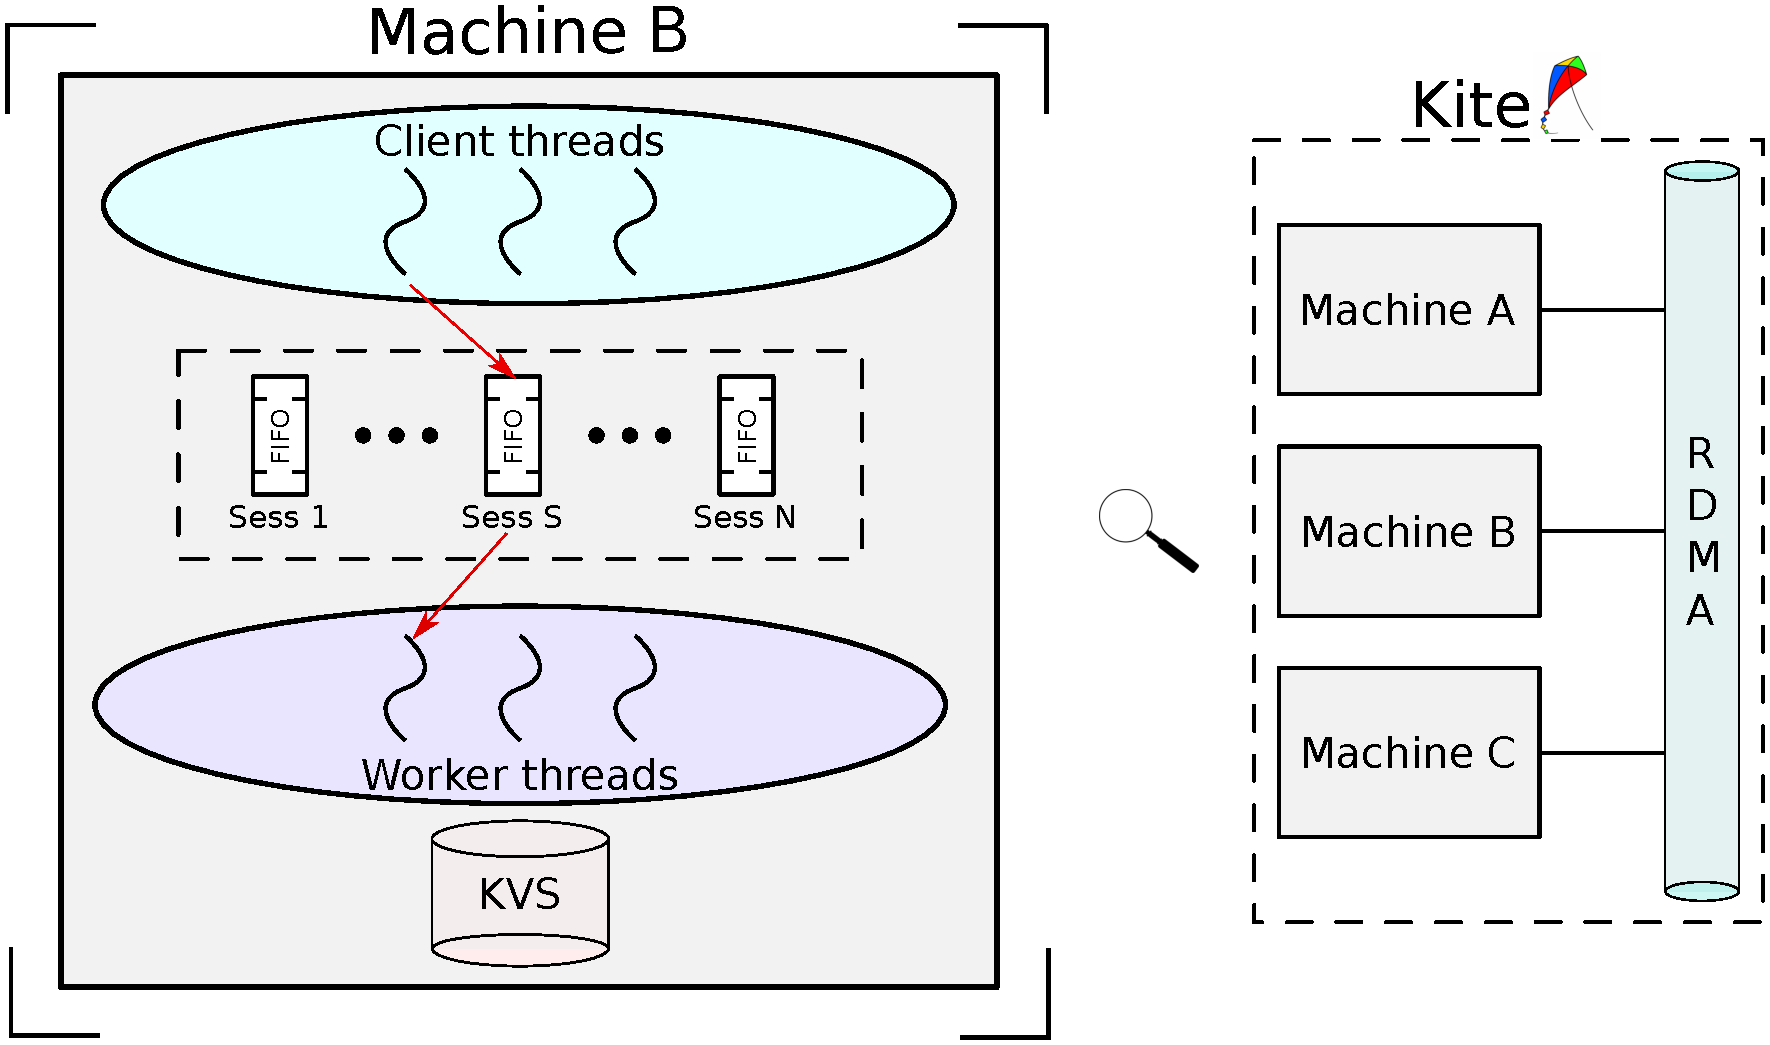
\includegraphics[scale=0.25]{1_figures/Wrkr-clt-Interface.pdf}
%   \vspace{-0.5em}
  \caption{A Kite machine is composed of worker and client threads, that interface through the session FIFOs.}
%   \vspace{-1.5em}
  \label{fig:interface}
\end{figure}


The \odlib~API offers reads, plain writes, and two types of conditional writes: 1) Fetch-\&-Add (FAA), and 2) Compare-\&-Swap (CAS).
%: a weak variant that can complete locally if the comparison fails locally, and a strong variant that always checks remote replicas.  
The \odlib~API includes an asynchronous (\emph{async}) and a synchronous (\emph{sync}) function call for every request (similarly to Zookeeper~\cite{Hunt:2010}). 


\beginbsec{Synchronous API } 
A sync call issues the request and then blocks polling for the request's completion.
We provide here the function call that issues a sync read:
\begin{lstlisting} 
sync_read(key_id, val_len, *value_ptr, session_id)
\end{lstlisting}
The programmer provides the key to be read ($key\_id$), the size of the value in bytes ($val\_len$), a pointer where the value should be copied ($*value\_ptr$) and the session id ($session\_id$). The call returns an integer, which, if 
negative, maps to an error code.
Sync calls simplify programming, but are not very efficient, as the client may need to block for several microseconds waiting for a request to complete. 

\beginbsec{Async API } An async call returns immediately before the request has completed. The client can call a polling function to find out if the request has been completed. As an example, we provide here the async read call:
\begin{lstlisting} 
async_read(key_id, val_len,  *value_ptr, session_id)
\end{lstlisting}
The call returns an integer, which, if negative, maps to an error code; otherwise, the returned integer denotes the \emph{request id} that can be used by the client to poll for the request's completion. \odlib~provides a range of  polling functions, that typically require a session id and a request id as arguments. 
\end{comment}
\begin{comment}
\beginbsec{Batched Asynchronous Programming }
Despite its performance benefits, an asynchronous API is admittedly quite cumbersome to program with.
For that reason, we make the following simplification: completed requests can only be polled in session order, irrespective of the order in which the worker completes them. This enables the client thread to issue a batch of requests and then at a later time, poll only for the last request issued.
If the last request is successfully polled, it guarantees that all preceding requests have been completed. We found this pattern very natural in porting code to \odlib.



\beginbsec{Multiple sessions per client thread} 
A client thread can use multiple sessions to improve performance: enabling thread-level parallelism across the workers, and session-level parallelism within one worker thread. 
Programmers can leverage this feature to parallelize their applications, by allocating parallelizable
tasks to different sessions. We leverage this capability when porting lock-free data structures to \odlib, 
in order to allow clients threads to work on multiple distinct operations concurrently, through different sessions. 


\beginbsec{Session FIFO}
Session FIFOs constitute the communication medium between client and worker threads. There can be thousands of sessions FIFOs (one per session), where each session maps to exactly one client and one worker thread. Therefore, any given session FIFO can only be accessed by one worker and one client. 
We focus on one slot of a single session FIFO. 
The slot's fields are illustrated in Figure~\ref{fig:fsm}a. The client fills the fields of the slot to issue a request, and the worker uses the fields to complete the request. For instance, on a CAS request the worker writes the result in the \emph{rmw result} field. If the CAS is unsuccessful, the worker also writes the read value in the address pointed to by the \emph{read value ptr} field.


\beginbsec{Request FSM} A FIFO slot contains a \emph{state} variable, which is used to facilitate the synchronization between worker and client. The state variable works as an Finite State Machine (FSM) (Figure~\ref{fig:fsm}), transitioning between four possible states, denoting who can access the slot. A client issues a request to the slot only if the state is \emph{Invalid}; issuing the request transitions the state to \emph{Active}, which implicitly passes the ownership of the slot to the worker thread. The worker will transition the slot to \emph{In-progress} when it polls it and later to \emph{Completed} when it completes it.


\begin{figure}[t]
   \centering
  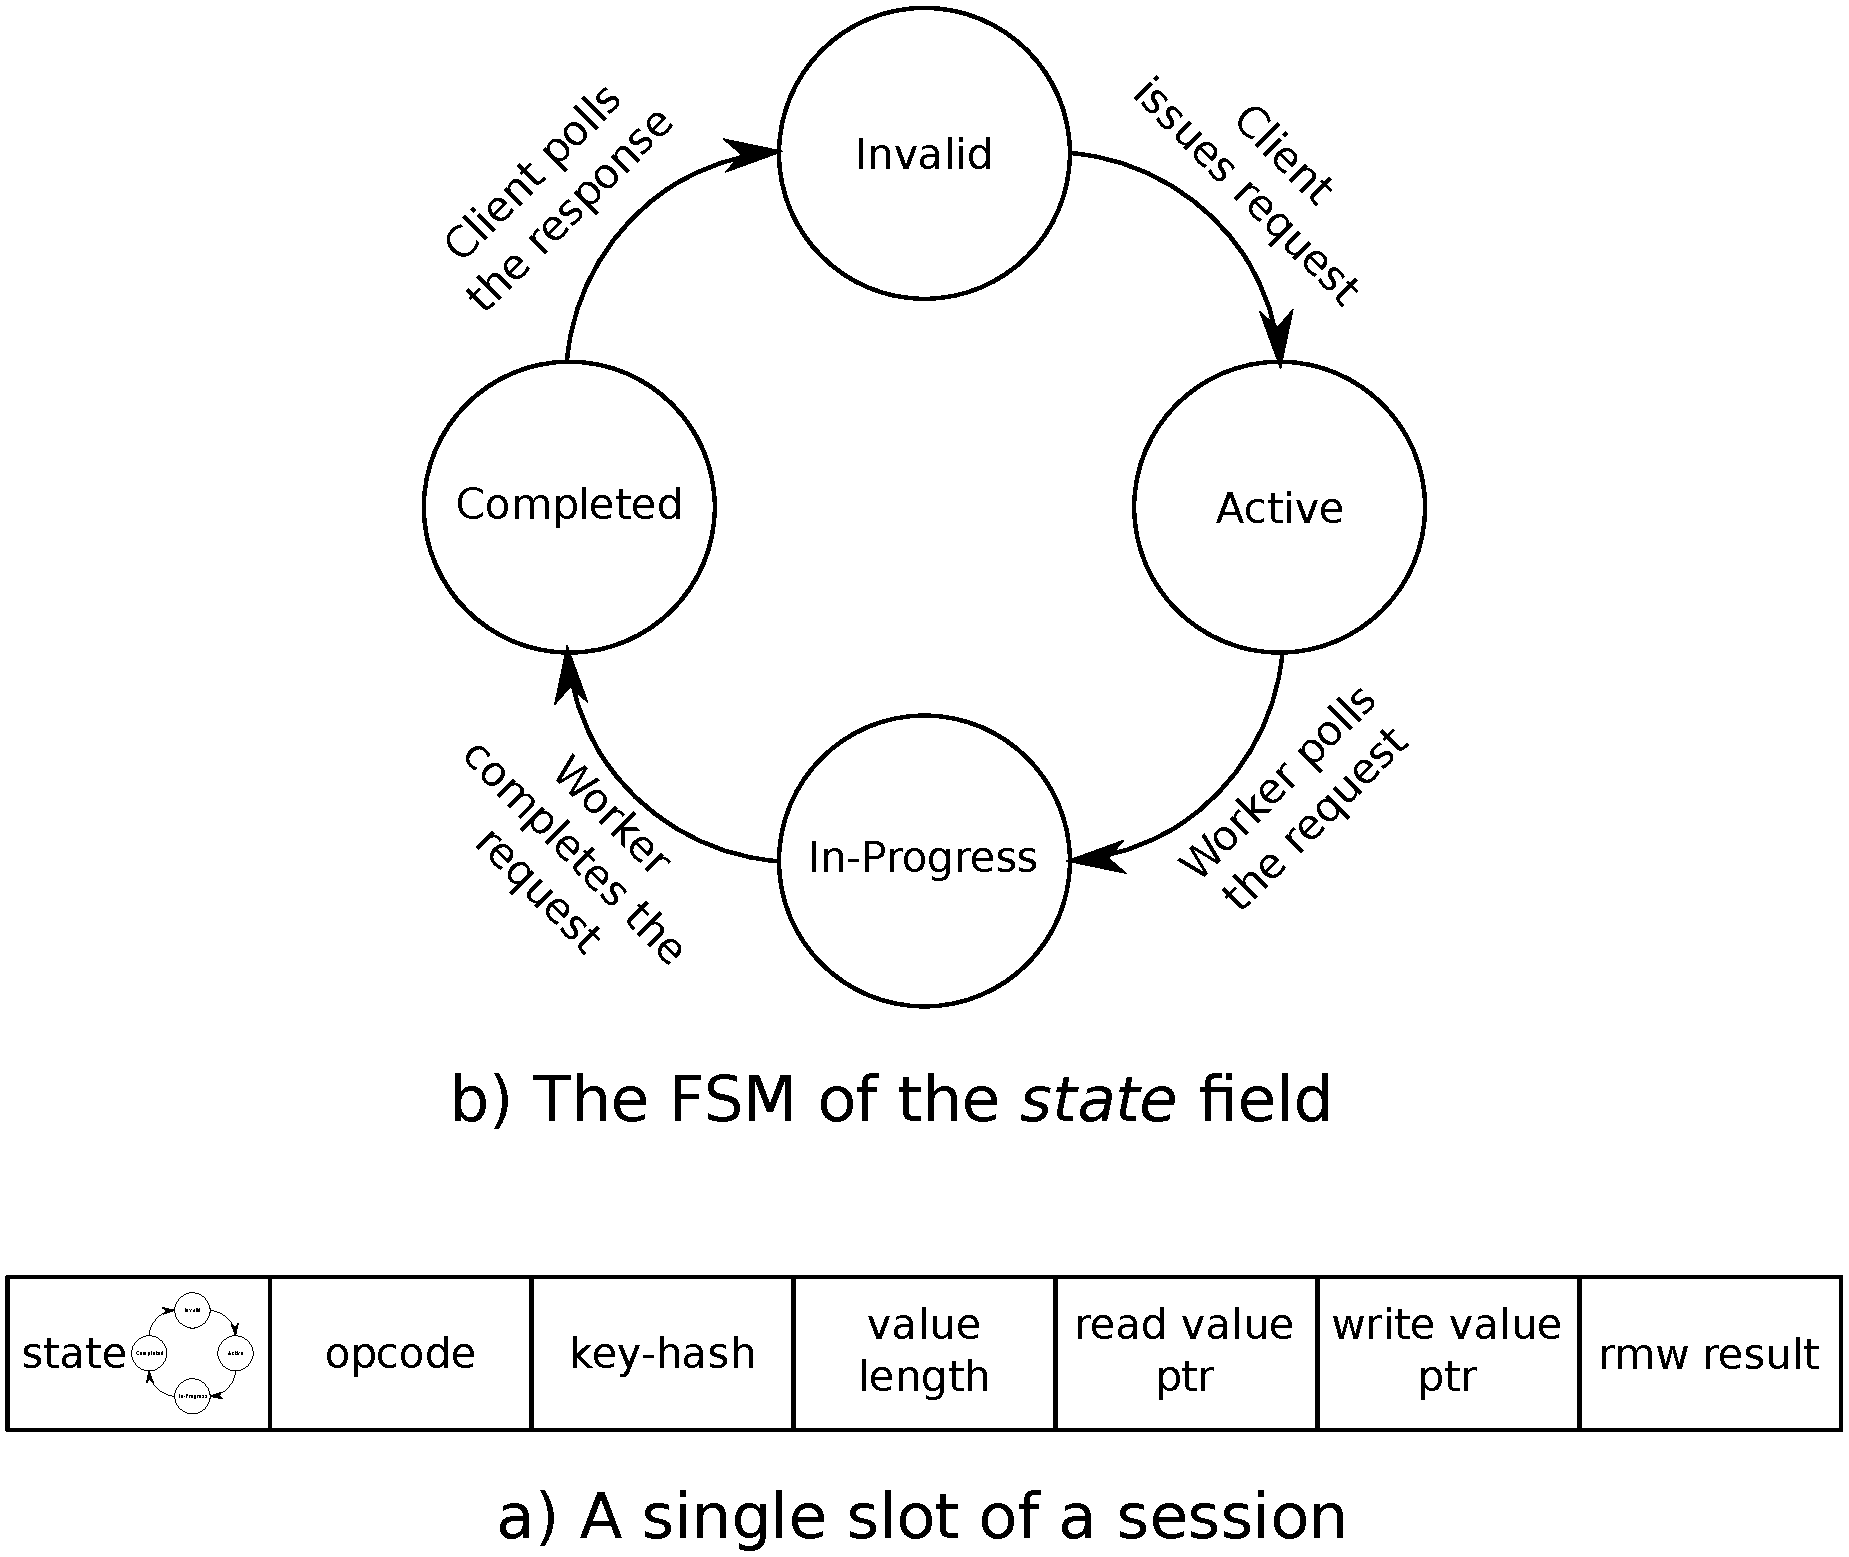
\includegraphics[scale=0.25]{1_figures/state-FSM.pdf}
  %\vspace{-1.5em}
  \caption{The fields of one slot of one session FIFO, and the FSM of the state field.}
  \label{fig:fsm}
\end{figure}
\end{comment}
\section{Infrastructure and workload}
\label{sec:meth}

% In this section we describe several parameters of our experiments.

% \beginbsec{Infrastructure}
We conduct our experiments on a cluster of 5 servers interconnected via a 12-port Infiniband switch (Mellanox MSX6012F-BS). Each machine runs Ubuntu 18.04 and is equipped with two 10-core CPUs (Intel Xeon E5-2630v4) with two hardware threads per core, reaching a total of 40 hardware threads. 
Furthermore each machine has 64 GB of system memory and a single-port 56Gb Infiniband NIC (Mellanox MCX455A-FCAT PCIe-gen3 x16). % connected on socket 0. 
% Each CPU has 25 MB of L3 cache and two hardware threads per core.
We disable turbo-boost, pin threads to cores and use huge pages (2 MB) for the KVS. 

% \beginbsec{Workload}
Our experiments use a uniform read/write trace, which is created on each run and is kept in-memory.
The KVS consists of one million key-value pairs, which are replicated in all nodes. We use keys and values of $8$ and $32$ bytes, respectively. 
%The requests are issued from the client threads over the async API.


\begin{comment}
The availability penalty need not be as big in this case, because the cost of a false positive is not as big: on a timeout, the leader is not removed from the configuration, but rather only voted out. 
\end{comment}

\section{Evaluation}
\label{sec:ev}

In this section, we analyze the performance of the \pnum~protocols that we have implemented over \odlib.
% Whenever necessary, we will discuss modifications the protocols to improve their thread-scalability, implement reads and match them with the KVS. We will discuss such modifications as we go along.
We start the discussion by providing a high-level overview of the 
%performance of the protocols. 
key insights of this evaluation.
Then we individually analyze the performance of each class of protocols. 
%In \secref{sec:ev:mcast}, we describe the impact of the hardware multicast primitive (introduced in \S\ref{sec:nw:mcast}).

\subsection{Overview} 
% (\figref{fig:three-bars} \& \tabref{tab:all-perf})}
\label{sec:ev:ov}

\begin{figure*}[t]
\centering
  \begin{subfigure}[b]{0.33\textwidth}
    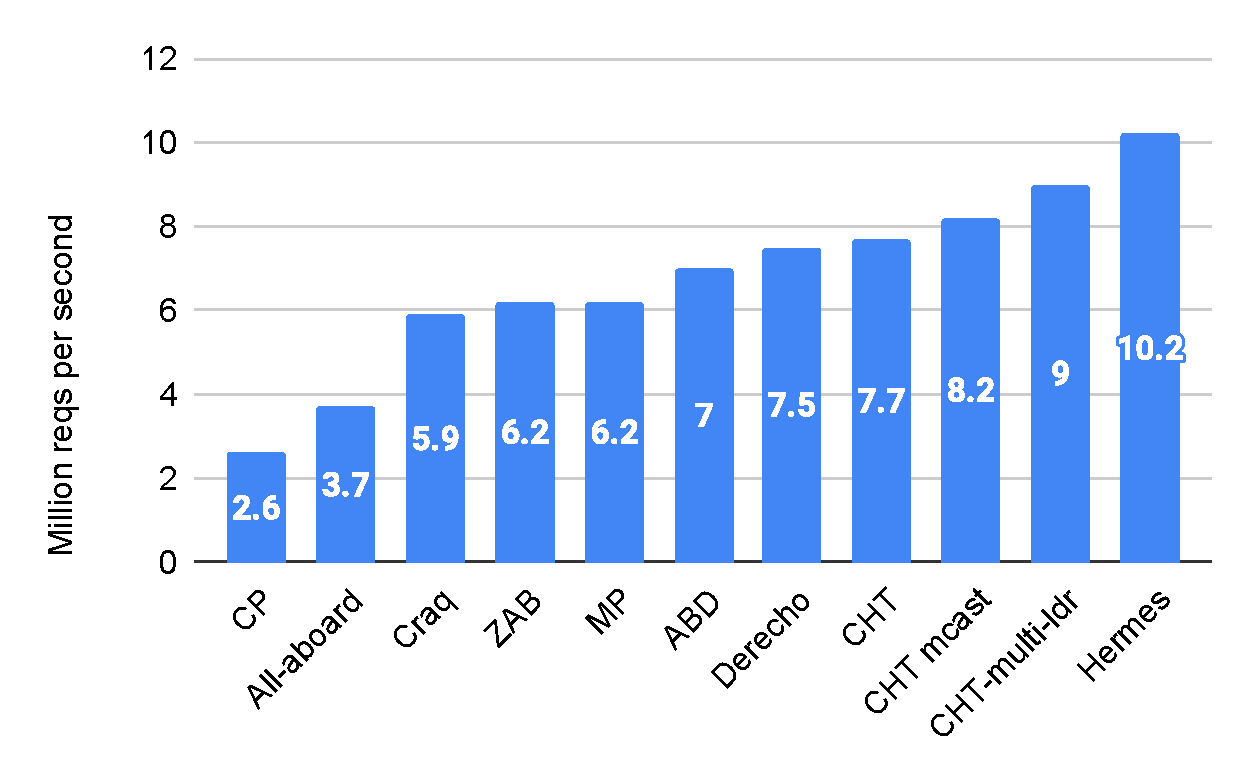
\includegraphics[width=\textwidth]{1_figures/single-thread.pdf}
    % \captionsetup{width=0.85\linewidth}
    % \vspace{-1.8em}
    \caption{Single-threaded write throughput}
%   \vspace{-1.5em}
  \label{fig:single-thr}
  \end{subfigure}
  %
  \begin{subfigure}[b]{0.33\textwidth}
    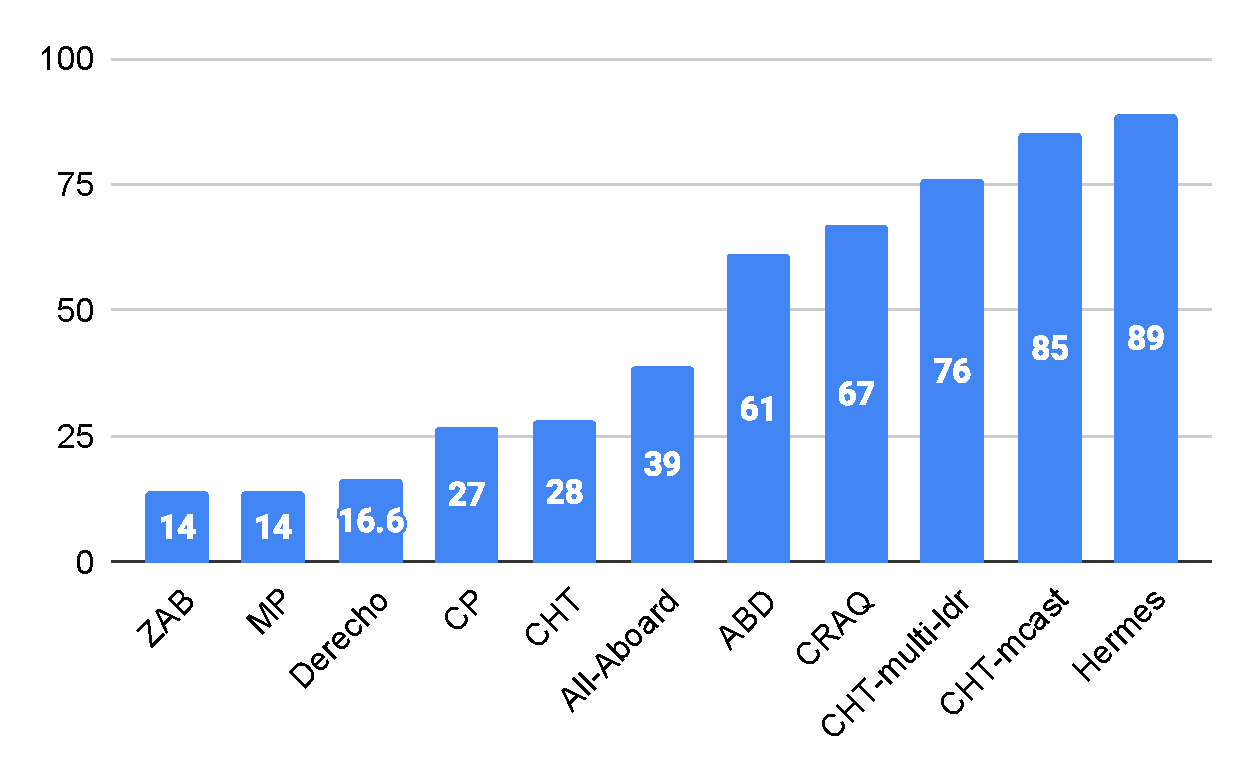
\includegraphics[width=\textwidth]{1_figures/Write-only-chart.pdf}
    % \captionsetup{width=0.85\linewidth}
    % \vspace{-1.8em}
    \caption{Multi-threaded write throughput}
    %   \vspace{-1.5em}
  \label{fig:write-all}
  \end{subfigure}
  %
  \begin{subfigure}[b]{0.33\textwidth} 
  
    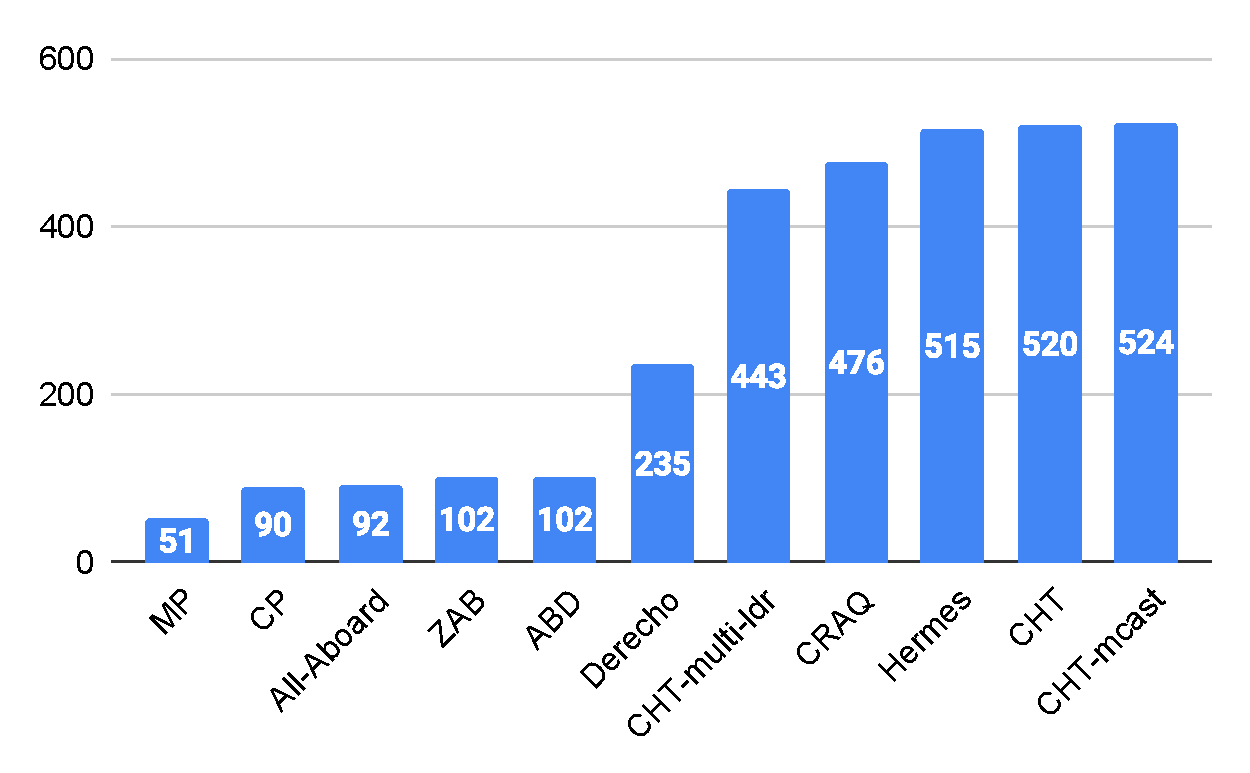
\includegraphics[width=\textwidth]{1_figures/5perc-writes.pdf}
    % \captionsetup{width=0.85\linewidth}
    % \vspace{-1.8em}
    \caption{Multi-threaded throughput at 95\% reads}
%   \vspace{-1.5em}
  \label{fig:5perc}
  \end{subfigure}
%   \vspace{-1em}
  \caption{Throughput comparison of all protocols in M.reqs/s. Note that both the x-axes and y-axes are different in each graph.}
 %\antonis{caption is closer to the text below than the subcaptions above}}
  \label{fig:three-bars}
%   \vspace{-1em}
\end{figure*}
% \begin{figure*}[t]
\centering
  \begin{subfigure}[b]{0.33\textwidth}
    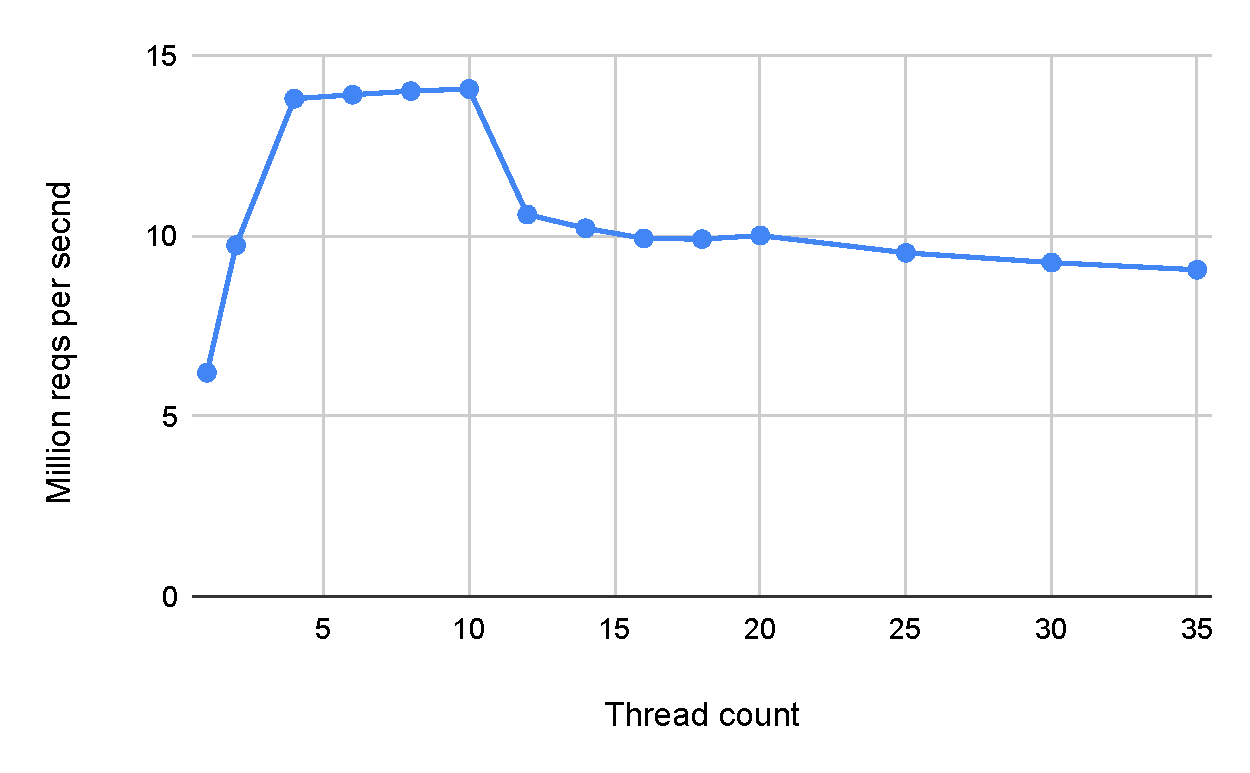
\includegraphics[width=\textwidth]{1_figures/ZAB-scal.pdf}
    \captionsetup{width=0.85\linewidth}
    % \vspace{-1.8em}
    \caption{Write-only throughput vs. thread cound for ZAB and MP}
%   \vspace{-1.5em}
  \label{fig:zab-scal}
  \end{subfigure}
  %
  \begin{subfigure}[b]{0.33\textwidth}
    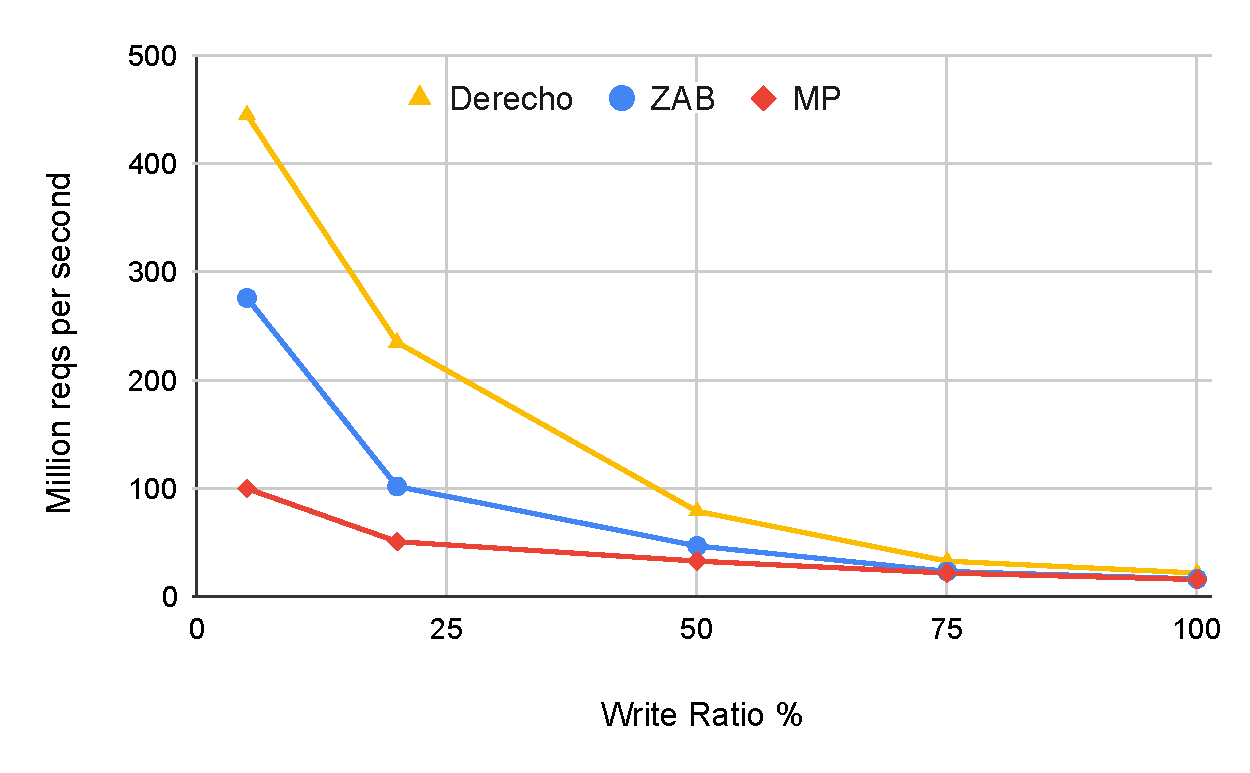
\includegraphics[width=\textwidth]{1_figures/zab-mp-dr.pdf}
    \captionsetup{width=0.85\linewidth}
    % \vspace{-1.8em}
    \caption{Throughput vs. write ratio for ZAB, MP \& Derecho}
    % \vspace{-1.5em}
  \label{fig:zab-mp-dr}
  \end{subfigure}
  %
  \begin{subfigure}[b]{0.33\textwidth} 
  
    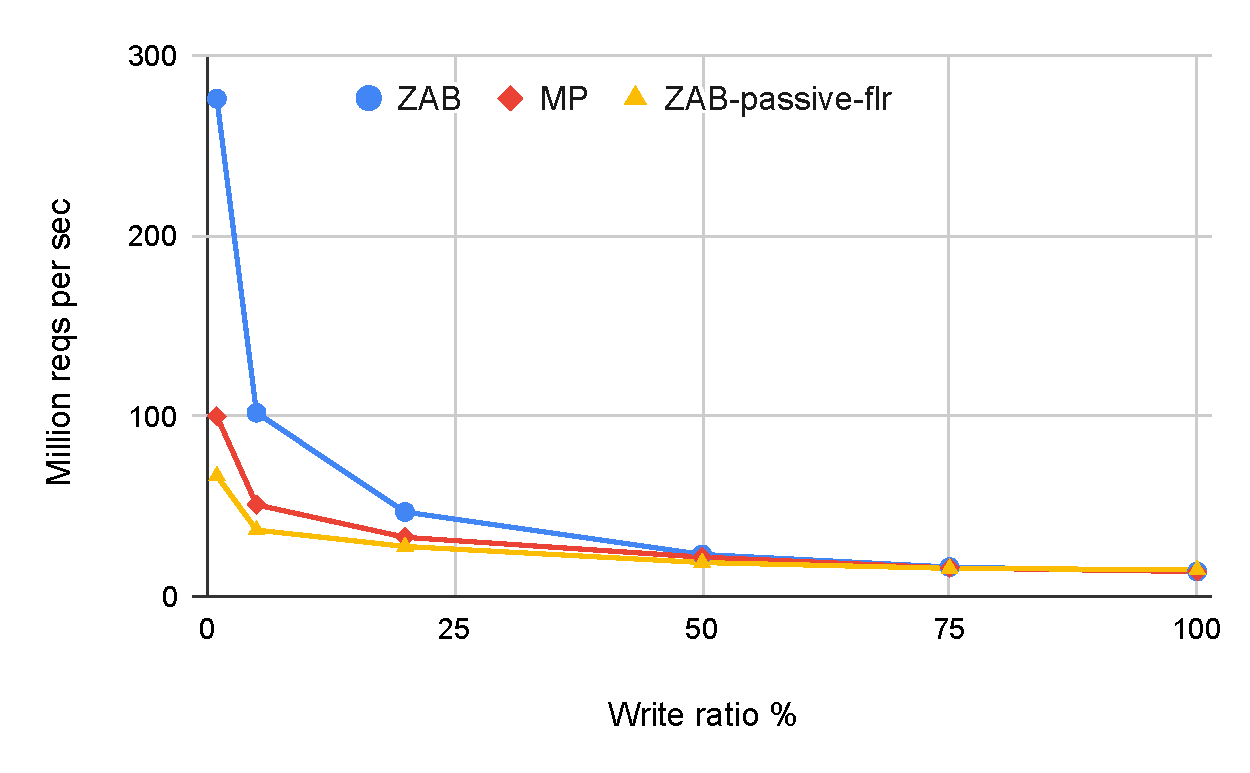
\includegraphics[width=\textwidth]{1_figures/zab-passive-flr.pdf}
    % \captionsetup{width=0.85\linewidth}
    \vspace{-1.8em}
    \caption{Throughput vs. write ratio for ZAB, MP and ZAB/MP with passive followers}
%   \vspace{-1.5em}
  \label{fig:zab-psv}
  \end{subfigure}
%   \vspace{-1em}
  \caption{Comparing ZAB, MP \& Derecho}
  \label{fig:lto}
%   \vspace{-1em}
\end{figure*}


% \begin{figure*}[t]
% \centering

% \begin{subfigure}[b]{0.33\textwidth}
%     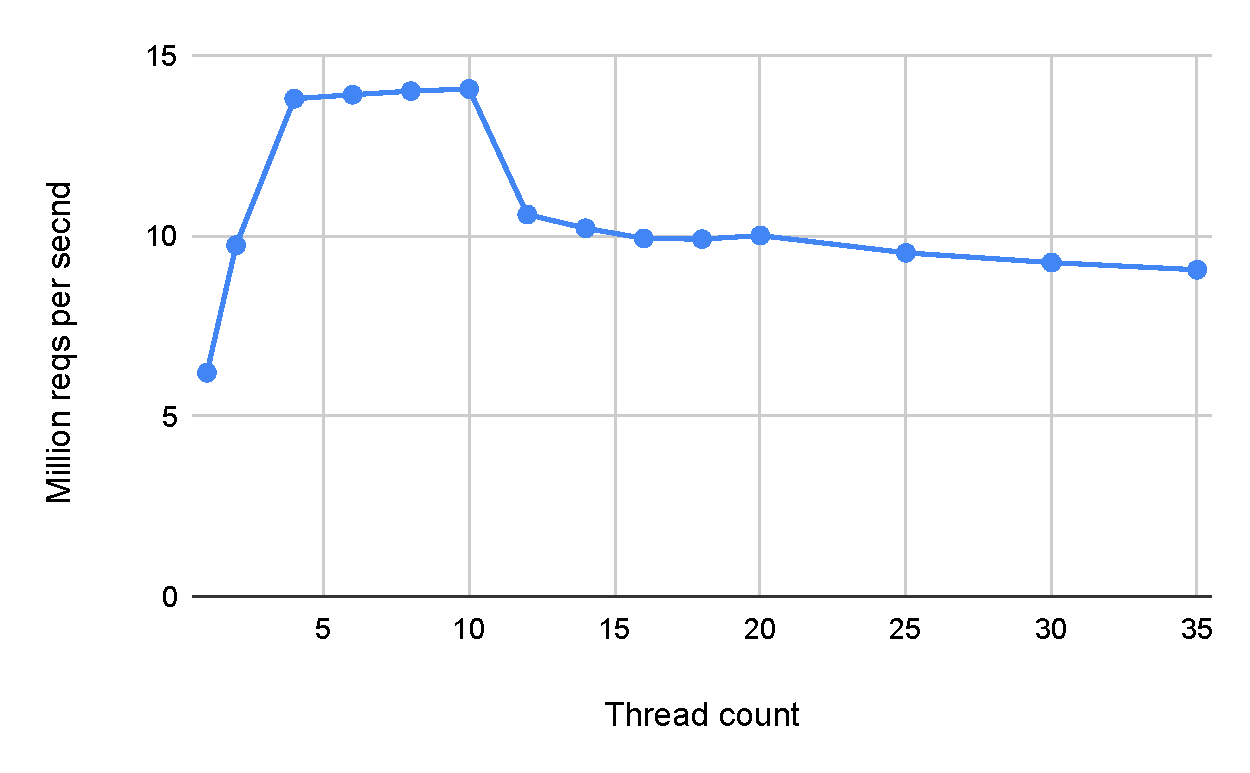
\includegraphics[width=\textwidth]{1_figures/ZAB-scal.pdf}
%     % \captionsetup{width=0.85\linewidth}
%     % \vspace{-1.8em}
%   \caption{Write-only throughput of ZAB and MP, varying the workers}
% %   \vspace{-1.5em}
%   \label{fig:zab-scal}
%   \end{subfigure} %%
  
% \begin{subfigure}[b]{0.33\textwidth}
% 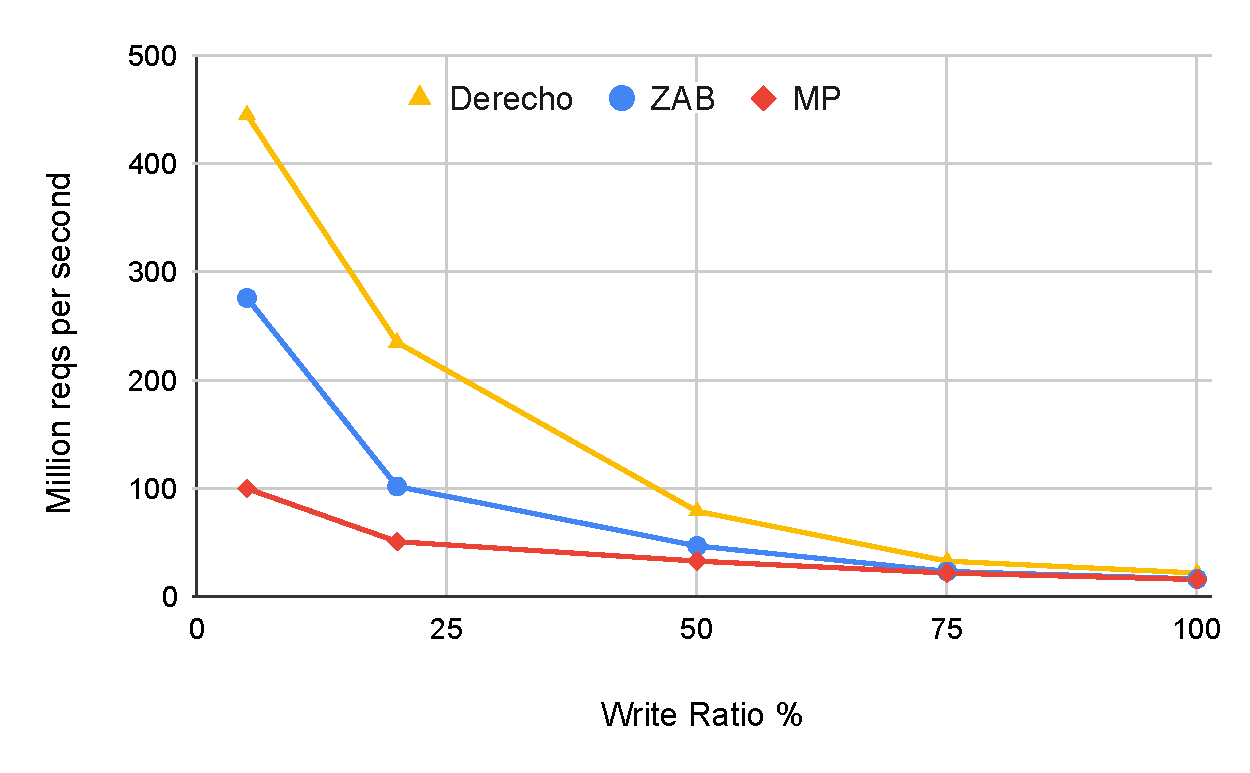
\includegraphics[width=\textwidth]{1_figures/zab-mp-dr.pdf}
% % \captionsetup{width=0.85\linewidth}
% % \vspace{-1.8em}
% \caption{Throughput of ZAB, MP \& Derecho, varying the write ratio from 1\% to 100\%}
% %   \vspace{-1.5em}
% \label{fig:zab-mp-dr}
% \end{subfigure}%

% \begin{subfigure}[b]{0.33\textwidth} 

% 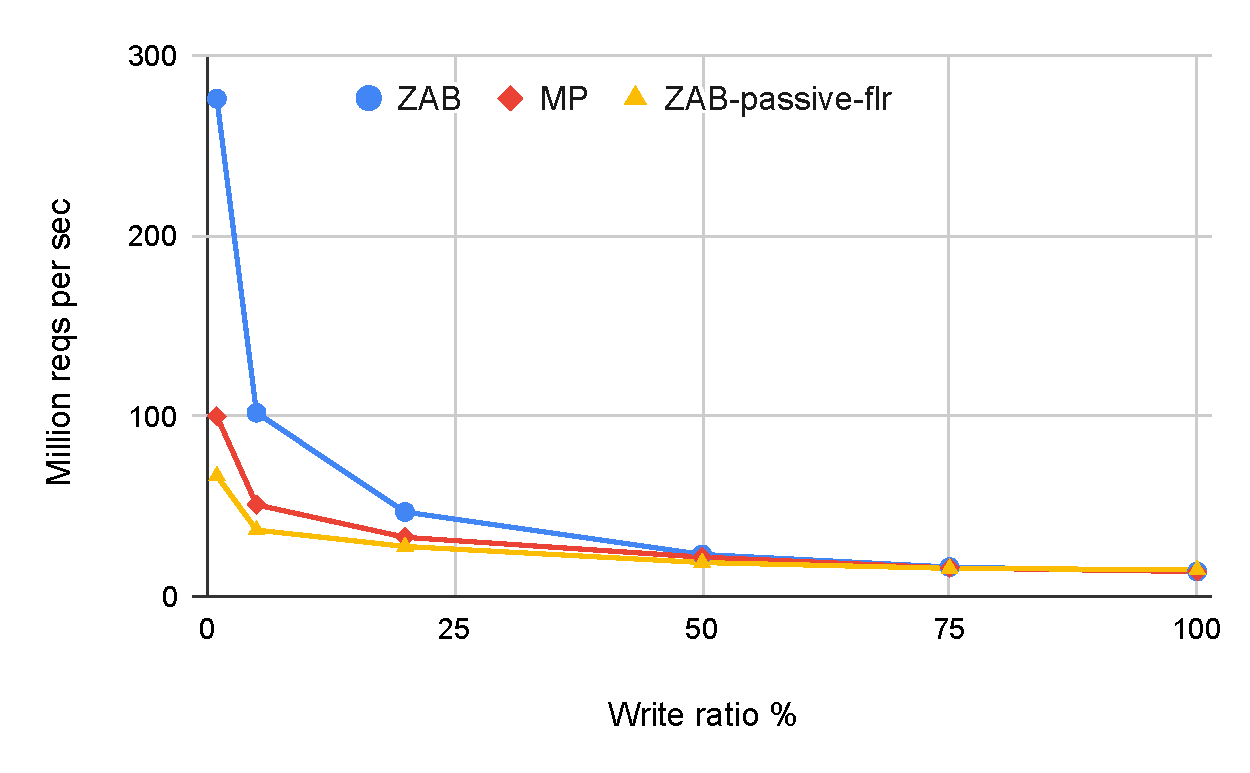
\includegraphics[width=\textwidth]{1_figures/zab-passive-flr.pdf}
% %   \vspace{-0.5em}
% \caption{Throughput of ZAB, MP and ZAB/MP with passive followers, when varying the write ratio}
% %   \vspace{-1.5em}
% \label{fig:zab-psv}
% \end{subfigure}%
% %   \vspace{-2em}
% \caption{\LTO~graphs. }
% \label{fig:lto}
% %   \vspace{-1.5em}
% \end{figure*}

First, we briefly describe \figref{fig:three-bars} and \tabref{tab:all-perf} and then analyze our key insights and provide general directives and recommendations. 

\beginbsec{\figref{fig:three-bars}}
\figref{fig:three-bars} shows the throughput of all protocols in million requests per second (M.reqs/s), ordering the protocols in ascending throughput order. 
% \figref{fig:single-thr} shows the order when the protocol are single-threaded, \figref{fig:write-all} when they are multi-threaded (the default case), and 
Specifically, \figref{fig:single-thr} and \ref{fig:write-all} show the write throughput of the protocols when they are single-threaded and multi-threaded (default scenario), respectively.
% \figref{fig:write-all} shows the same write throughput when protocols are multi-threaded (default scenario).
Finally, \figref{fig:5perc} shows the throughput (multi-threaded), with 95\% reads.




Note the following three remarks for \figref{fig:three-bars}.
Firstly, both the x-axis and y-axis are different in all three graphs. Crucially, protocols in the x-axis are ordered in ascending throughput order.
% to highlight their performance relation
Secondly, MP and ZAB are the same protocol in the write-only workload, \ie in \figref{fig:single-thr} and \ref{fig:write-all}, because they only differ in the execution of reads.
Third and final, note that there is a protocol called \emph{CHT-mcast}: this is the CHT protocol with the hardware multicast enabled. We show its performance separately because it performs significantly better than CHT. Enabling the multicast in the rest of the protocols has a very small impact. %, and we discuss why in Section~\secref{sec:ev:mcast}.

\beginbsec{\tabref{tab:all-perf}}
The left-hand side of \tabref{tab:all-perf} shows the throughput in M.reqs/s of all protocols when varying the write ratio. 
% Throughout this section, we plot the throughput measurements from this table whenever necessary.
The right-hand side shows the latency (99th / average) of all protocols in microseconds at 100\% write ratio, while varying the load of the protocol (\ie with respect to peak throughput). 
% In ZAB, MP and CHT variants, we have measured the latency at a follower node. In CRAQ, we have measured the latency at the head node.

\custvspace
\noindent
Let us now summarize the key insights from this study.

% \beginbsec{Observations}

\beginbsec{1. Total order is not thread-scalable}
Protocols that apply writes in a total order are not thread-scalable:
the relative positions of ZAB, MP (\LTO), and Derecho (\DTO) in \figref{fig:single-thr} and \figref{fig:write-all} demonstrate this point. The reason is that explicitly enforcing total order mandates that threads can only apply writes to the KVS in lock-step.
In contrast, protocols that enforce per-key order (\LPKO~and \DPKO) can scale well with more threads.

\beginbsec{2. The leader jeopardizes load balance}
The adverse effect of the leader on load balance is not apparent in \LTO~protocols because they cannot scale enough to uncover it.
However it is visible in \LPKO~protocols.
% \LPKO~protocols, struggle to achieve load balance. 
Specifically, CHT does not scale well when multi-threaded because the send side of the leader becomes the bottleneck. % as the leader is responsible for broadcasting every write.
There are two protocol-level optimizations that restore load balance: propagating writes through a chain (\ie CRAQ) and using multiple leaders (\ie CHT-multi-ldr).
% Finally, we expose a third optimization using the hardware multicast primitive (\ie CHT-mcast). In \secref{sec:}, we explain how multicast makes a leader-based protocol as efficient as a decentralized protocol such as Hermes.

\beginbsec{3. Hardware multicast is effective for \LPKO}
The hardware multicast primitive can make a huge difference, but only in \LPKO~protocols.
Specifically, the hardware multicast primitive provides a 3x benefit for CHT, i.e., CHT-mcast. 
The benefit for the rest of the protocols is very small, typically around 5\%.
The reason is that the multicast only relieves load on the send side of the node that performs the broadcast: it reduces the number of messages sent, but not the number of messages received.
Therefore, multicast is extremely useful for leader-based protocols that are bottlenecked by the send bandwidth of the leader. It is not so useful for already well-balanced protocols (\ie \DTO\  and \DPKO), while \LTO\ protocols do not benefit, as they are already bottlenecked by thread-scalability. We will expand in \secref{sec:ev:lpko}.% This is highlighted by the performance of CHT-mcast, which removes that bottleneck by using the multicast primitive.
% CRAQ and CHT-multi-ldr which explicitly target load balance also achieve very good performance.

\beginbsec{4. \DPKO~excels when multi-threaded}
In the absence of a leader or a total order, \DPKO\ protocols must find creative ways to serialize writes in a decentralized manner.
% \DPKO~protocols have a high work-per-request ratio, because in the absence of a leader or a total order, they must find creative ways to serialize writes.
On the one hand, this invites a level of complexity that has an adverse affect on the work-per-request ratio. 
This is portrayed by the single-threaded performance of CP and All-Aboard, which is the lowest among all protocols.
On the other hand, the decentralized nature of these protocols makes them
naturally thread-scalable and load balanced. This is why multi-threading yields a $\sim$9-10x throughput improvement.
Notably, by downgrading the availability guarantees, as in Hermes, or downgrading the API, as in ABD, it is possible reduce the work-per-request ratio.

\beginbsec{5. Thread-scalability > load balance > work-per-request}
From \figref{fig:write-all}, we observe that the non-thread-scalable protocols, ZAB, MP and Derecho are the worst performers, rendering thread-scalability the most critical property to honour in the modern era.
Furthermore, All-Aboard, a protocol with a very high work-per-request ratio, significantly outperforms CHT, which sacrifices load balance, even though CHT offers lower availability guarantees (discussed in \S\ref{sec:fail}).
From that we concur that it is preferable to optimize for load balance rather than work-per-request ratio. At the limits of the work-per-request ratio (\ie in CP), the two metrics appear equally important, as CHT and CP are roughly matched.



% However, \DPKO~protocols are also naturally thread-scalable and load balanced, which is why multi-threading yields a $\sim$9-10x throughput improvement---making CP, All-aboard, and ABD attractive design points for systems keen on favouring availability. 
% Hermes is the best-performing protocol in both \figref{fig:single-thr} and~\ref{fig:write-all}.
% That is because
% Hermes keeps the work-per-request low by mandating that every message must reach all machines. The cost of this choice is an availability penalty in case of a failure.

\beginbsec{6. Local reads are great but with caveats}
Recall that MP performs reads by sending them to the leader. CP, All-aboard and ABD perform ABD-reads (typically 1 broadcast round). The rest perform reads locally.
From \figref{fig:5perc}, we see that there is a big gap between protocols with local reads and the rest, which perform them remotely. However there are a couple of caveats.
Firstly, local reads always come at a cost as they downgrade either the consistency or the availability guarantees, as we saw in \secref{sec:fail}.
Furthermore, note that ZAB, even though it performs its reads locally, is on par with the protocols that perform reads remotely.
This is because it is bottlenecked by its write throughput.
We elaborate in \secref{sec:ev:lto}.
% Specifically, since ZAB's peak write throughput is 14 M.reqs/s, that means that its theoretical limit at 5\% writes is 280 M.reqs/s. In practice, ZAB reaches only 102 M.reqs/s
% The conclusion is that local reads are extremely beneficial, however, they can be bottlenecked by the write throughput in protocols that do not scale well.

% In fact, in the modern era we argue that the opposite is true: in order to optimize latency, one should actually prioritize thread-scalability and load balance.
% Here is why. With networking and memory accounting for a few microseconds, the request latency does not typically exceed a few tens of microseconds on a lightly loaded system. 
% Therefore, to ensure microsecond latency, we need only ensure that the system is not overloaded.
% This calls for high-throughput protocols as the target throughput is less likely to overload such protocols. 
% To maximize throughput,  thread-scalability and load balance should be prioritized over traditional metrics such as number of messages per request.
% Our evaluation corroborates this hypothesis (\S~\ref{sec:ev}).

\beginbsec{7. For better latency, choose throughput}
In the Introduction, we hypothesized that a request's latency should not exceed a few tens of microseconds in a lightly loaded system. 
Furthermore, we argued that to ensure a low latency, we should favour high-throughput protocols. %, as they will be less loaded at the target throughput.
The latency measurements for 25\% load in \tabref{tab:all-perf} verify that at a light load, all protocols incur a latency of a few tens of microseconds. 
Furthermore, we observe that for all protocols, as load increases so does latency, with a big spike at 100\% load. Therefore, to maintain a latency of a few tens of microseconds, 
%we need to ensure the protocol is not overloaded.
% To achieve that, 
one should favour high-throughput protocols, as they will be less likely to be overloaded when operating on the target throughput. %, and thus more likely to deliver a lower latency.
% In fact, using 
% In all cases, going from 25\% load to 75\% or 100\%  has a worse effect in latency than 
% %at a light load.
% All protocols see a big jump in latency when 100\% loaded.
% % However, for all protocols, as load increases so does latency.
% Therefore, to achieve the lowest latency, one should favour high-throughput protocols, as they will be less loaded when operating on the target throughput, and thus more likely to deliver a lower latency.
% For example, Hermes achieves roughly the same throughput at 25\% load as ZAB does at 100\% load.  but enjoying a significantly lower latency.
% For that reason
% Therefore, the protocol with the lowest load at the target throughput is the most likely to achieve the lowest latency. 
% Therefore, even when optimizing for latency, one should favour throughput, as high-throughput protocols will be less loaded at the target throughput.

% Note, however that Hermes achieves higher throughput at 25\% load than ZAB at 100\% load. Therefore, for the same throughput requirements, Hermes will enjoys a lower latency, simply because it is less loaded.
% This corroborates our hypothesis that for better latency, high-throughput protocols should be favoured.
% Furthermore, we argued that to maintain this low latency, we only needed to ensure that the system would not become overloaded. To achieve that we should favour high-throughput protocols, as they will be less loaded at the target throughput. Again, from 


% From the latency results in \tabref{tab:all-perf} we make the following observation.
% There is not a strong correlation between the work-per-request ratio and the latency of the protocols. Instead, the most impactful factor is the load imposed on a protocol. Specifically, all protocols incur a few microseconds at 25\% load, which grows to 100s of microseconds at 100\% load. 
% It is crucial to note that protocols with the same load achieve different throughput.
% For instance, Hermes achieves a higher throughput at 25\% load than ZAB at 100\% load. Therefore, for the same throughput requirements, Hermes enjoys a lower latency, simply because it is less loaded.
% Therefore, we recommend that a protocol is chosen based on its throughput capabilities. This will guarantee that the load on the protocol is always the lowest possible, which in turn yields the lowest latencies.


% \beginbsec{Conclusions}
% The conclusions of our evaluation are the following:
% Total order should always be avoided in read/write systems.
% Leader-based protocols can offer high-performance, but care must be taken to restore load balance.
% The hardware multicast primitive can make a huge difference but only in \LPKO~protocols.
% Local reads are very beneficial, but can be bottlenecked by the write throughput.
\beginbsec{Summary -- Recommendations}
Based on our insights, we first provide some general directives on protocol design and then offer recommendations on choosing a protocol.
% \fbox{
% \begin{minipage}{0.45 \textwidth}

\beginbsec{General Directives}
\squishlist
% Firstly, a few general directives.
\item %Among thread-scalability, load-balance and the work-per-request ratio, 
Prioritize thread-scalability, then load-balance and then the work-per-request ratio.
%Favouring thread-scalability is the most imporant concern. 
\item Total order should be avoided in read/write systems.
\item Leader-based protocols can achieve high-performance, but care must be taken to ensure load balance. 
\item It is worth investing in the hardware multicast primitive only in the case of \LPKO\ protocols. 
\item Local reads can deliver great performance, but it's not guaranteed.
%should be preferred for performance, but one should be wary of their cost.
\item In order to minimize latency, choose protocols with high throughput.
\squishend
% \beginbsec{Concrete Recommendations}
\noindent\textbf{Recommendations}
\squishlistContrib
\item All-aboard is the most attractive design point for a scenario where: 1) availability is the most important concern and 2) conditional writes are required.
\item If simple writes will do, then we recommend ABD.
\item If a small window of unavailability on a failure is tolerable, then Hermes is the best candidate, while CHT-multi-ldr and CRAQ are good alternatives.
\squishend 
% \end{minipage}
% }
\begin{comment}


\beginbsec{\tabref{tab:all-perf}: Throughput \& Latency}
The left-hand side of \tabref{tab:all-perf} shows the throughput in M.reqs/s of all \pnum~protocols (plus CHT-mcast) when varying the write ratio. 
Throughout this section, we plot the throughput measurements from this table whenever necessary.

The right-hand side shows the latency (99th / average) of all protocols in microseconds at 100\% write ratio, while varying the load of the protocol (\ie with respect to peak throughput). 
In ZAB, MP and CHT variants, we have measured the latency at a follower node. In CRAQ, we have measured the latency at the head node.
\end{comment}
\begin{comment}


\todo{I will write the part about latency, once i make another pass over the intro}
In \secref{sec:introduction}, we made a hypothesis and then based on that  a claim.
Our hypothesis was that 
there is not a strong correlation between the work-per-request ratio and the latency of the protocols. 
Our claim based on that was that the protocol designer should not try to minimize work-per-request at the expense of load balance or thread-scalability. Instead she should favour throughput in order to increase latency.

To test our hypothesis consider CP

It has the highest work-per-request ratio which includes three heavy broadcast rounds. 
However, its latency does not stand out. 
The reason is that with RDMA networking, sending a message takes only a few microseconds. 
However, the 99th percentile latency of CP at 100\% load is 216 microseconds. The dominant factor in that number is queuing. 
Queuing occurs as the request travels from buffer to buffer during its lifetime from the client thread to a worker thread, propagating to all nodes and coming back to the client. 

Now consider our claim. 
\end{comment}


\begin{figure*}[t]
\centering
  \begin{subfigure}[b]{0.33\textwidth}
    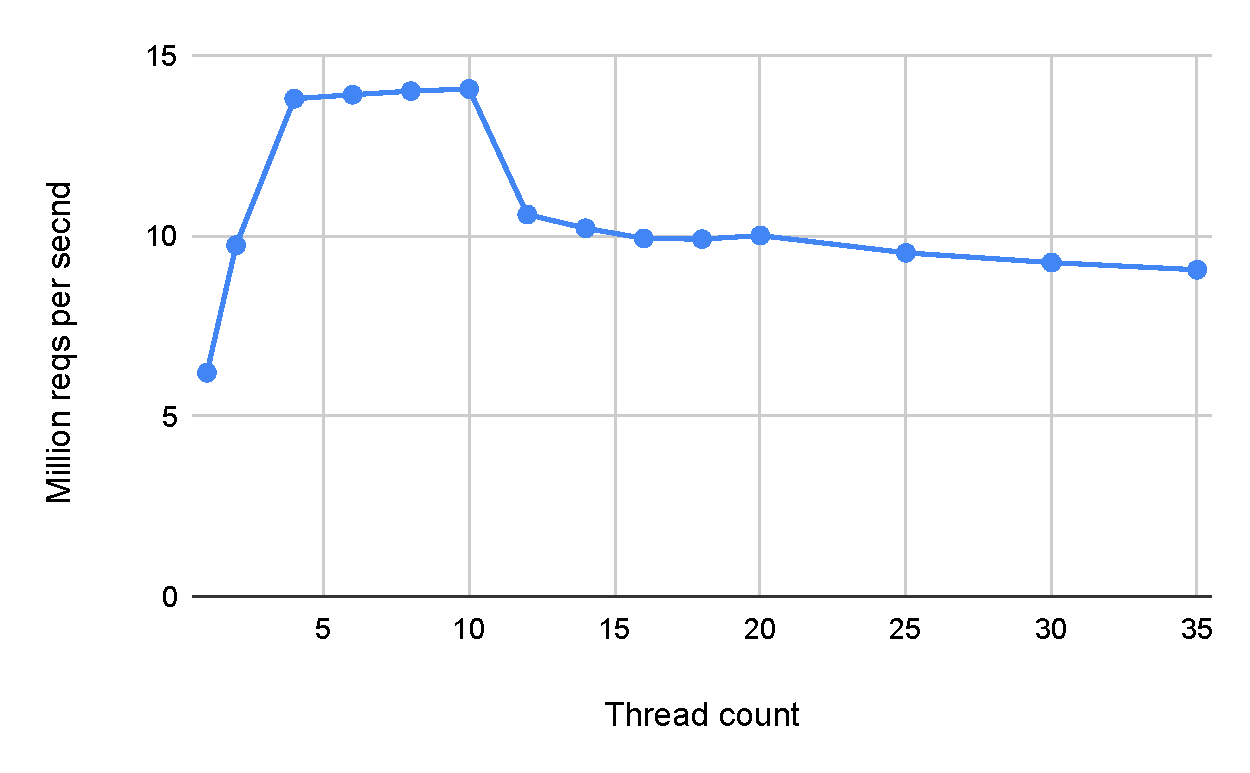
\includegraphics[width=\textwidth]{1_figures/ZAB-scal.pdf}
    \captionsetup{width=0.85\linewidth}
    % \vspace{-1.8em}
    \caption{Write-only throughput vs. thread cound for ZAB and MP}
%   \vspace{-1.5em}
  \label{fig:zab-scal}
  \end{subfigure}
  %
  \begin{subfigure}[b]{0.33\textwidth}
    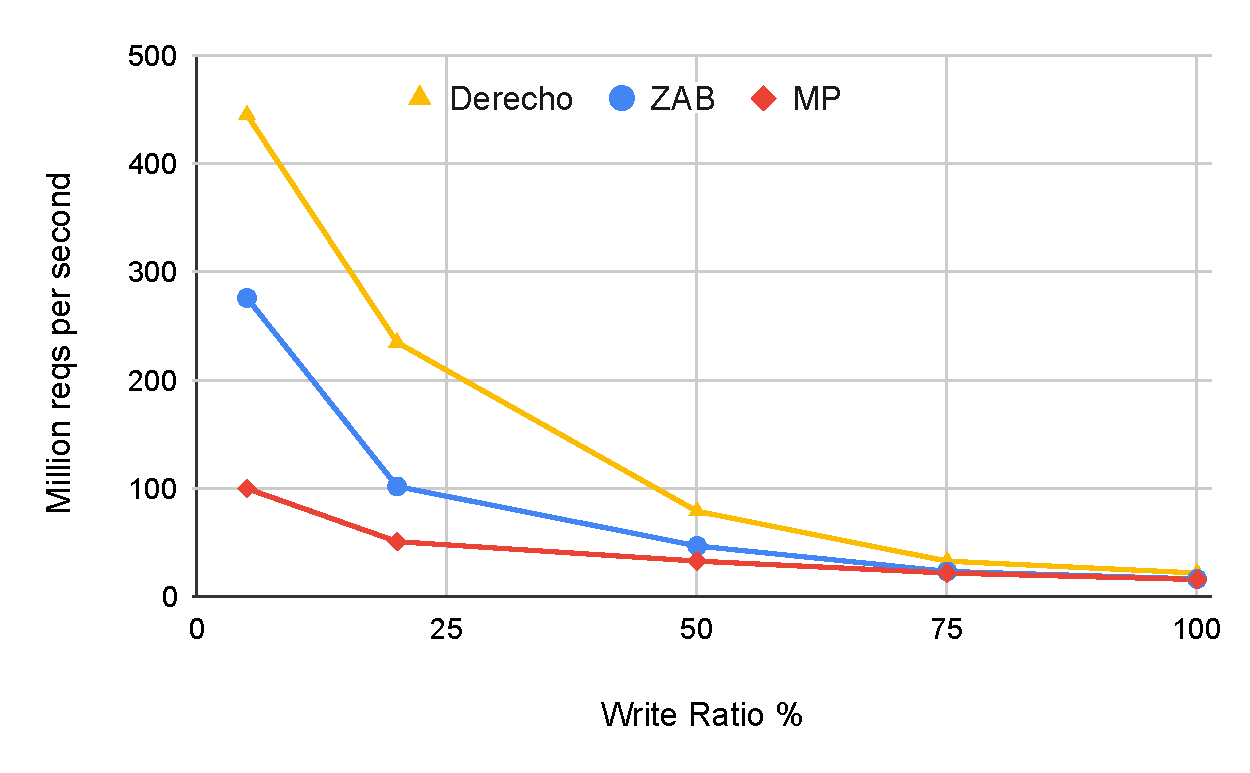
\includegraphics[width=\textwidth]{1_figures/zab-mp-dr.pdf}
    \captionsetup{width=0.85\linewidth}
    % \vspace{-1.8em}
    \caption{Throughput vs. write ratio for ZAB, MP \& Derecho}
    % \vspace{-1.5em}
  \label{fig:zab-mp-dr}
  \end{subfigure}
  %
  \begin{subfigure}[b]{0.33\textwidth} 
  
    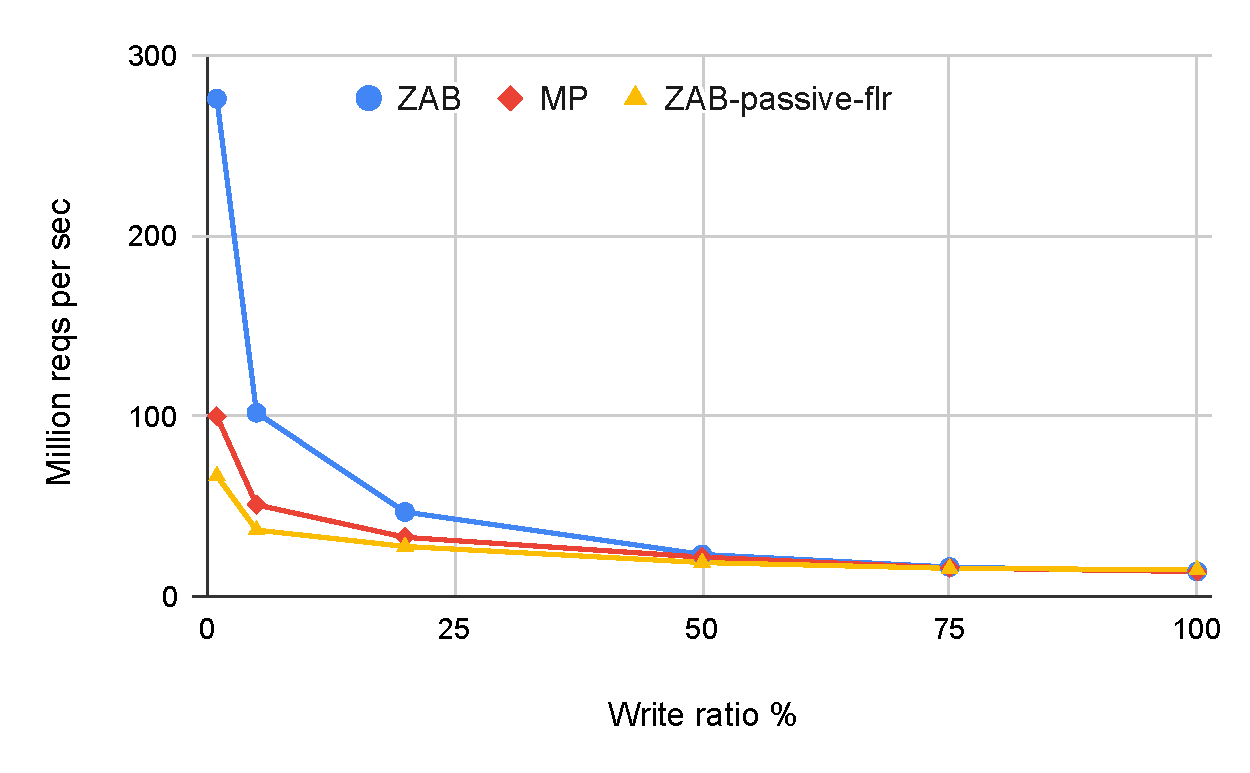
\includegraphics[width=\textwidth]{1_figures/zab-passive-flr.pdf}
    % \captionsetup{width=0.85\linewidth}
    \vspace{-1.8em}
    \caption{Throughput vs. write ratio for ZAB, MP and ZAB/MP with passive followers}
%   \vspace{-1.5em}
  \label{fig:zab-psv}
  \end{subfigure}
%   \vspace{-1em}
  \caption{Comparing ZAB, MP \& Derecho}
  \label{fig:lto}
%   \vspace{-1em}
\end{figure*}


% \begin{figure*}[t]
% \centering

% \begin{subfigure}[b]{0.33\textwidth}
%     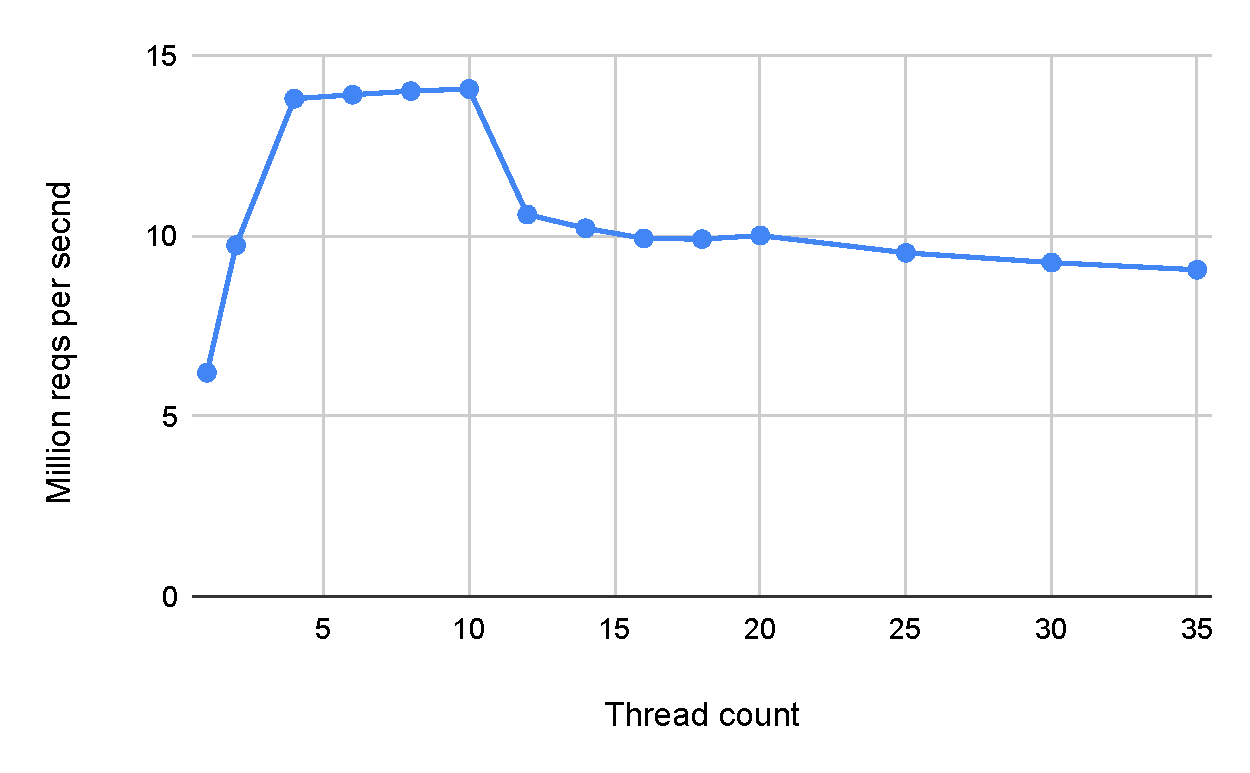
\includegraphics[width=\textwidth]{1_figures/ZAB-scal.pdf}
%     % \captionsetup{width=0.85\linewidth}
%     % \vspace{-1.8em}
%   \caption{Write-only throughput of ZAB and MP, varying the workers}
% %   \vspace{-1.5em}
%   \label{fig:zab-scal}
%   \end{subfigure} %%
  
% \begin{subfigure}[b]{0.33\textwidth}
% 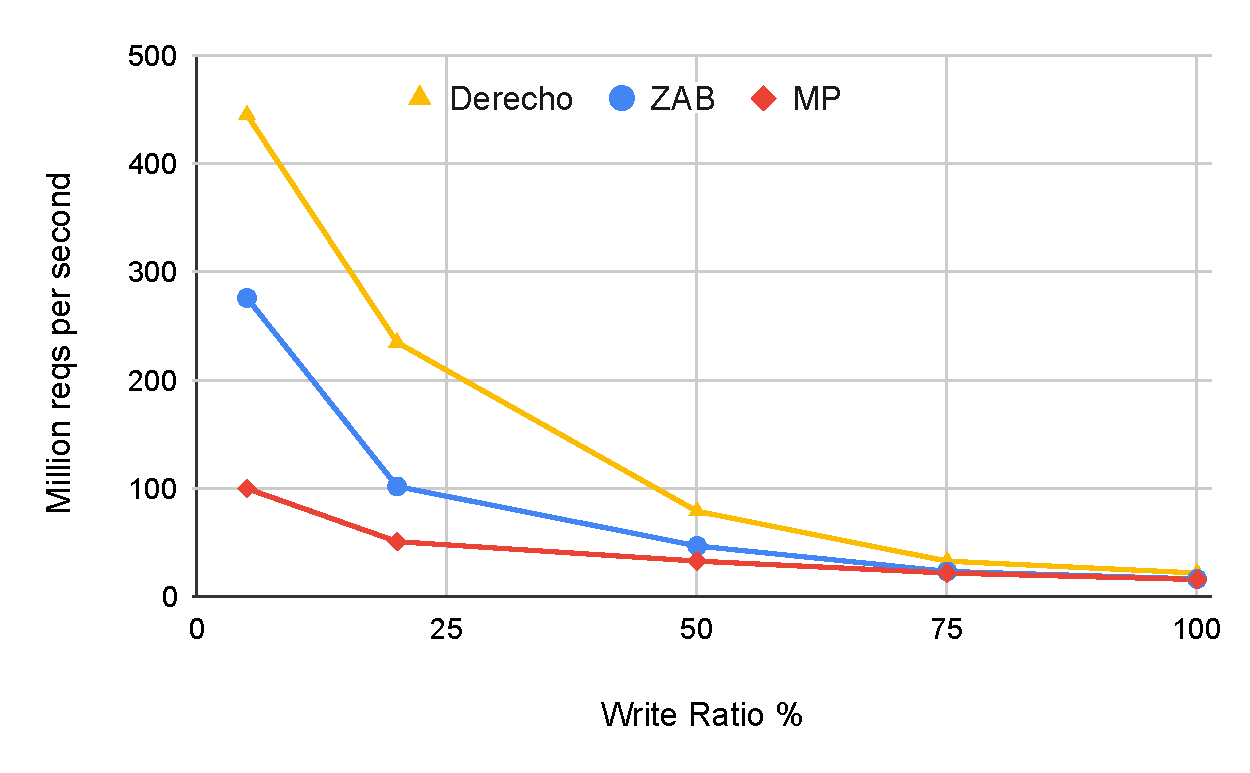
\includegraphics[width=\textwidth]{1_figures/zab-mp-dr.pdf}
% % \captionsetup{width=0.85\linewidth}
% % \vspace{-1.8em}
% \caption{Throughput of ZAB, MP \& Derecho, varying the write ratio from 1\% to 100\%}
% %   \vspace{-1.5em}
% \label{fig:zab-mp-dr}
% \end{subfigure}%

% \begin{subfigure}[b]{0.33\textwidth} 

% 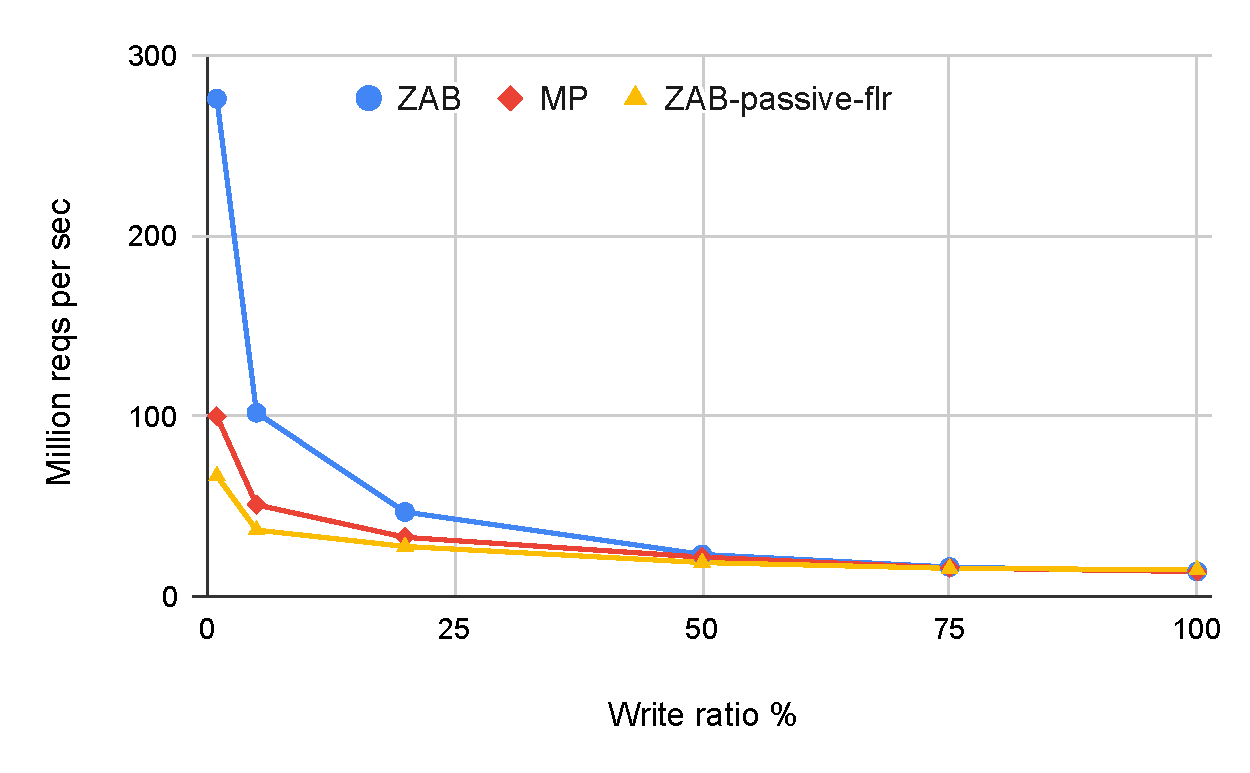
\includegraphics[width=\textwidth]{1_figures/zab-passive-flr.pdf}
% %   \vspace{-0.5em}
% \caption{Throughput of ZAB, MP and ZAB/MP with passive followers, when varying the write ratio}
% %   \vspace{-1.5em}
% \label{fig:zab-psv}
% \end{subfigure}%
% %   \vspace{-2em}
% \caption{\LTO~graphs. }
% \label{fig:lto}
% %   \vspace{-1.5em}
% \end{figure*}
\begin{table}[t]
\centering
 \resizebox{0.48\textwidth}{!}{%
\begin{tabular}{c|c|c|c|c|c|c|c|||c|c|c|c|c|}
\hhline{~-----------}
& \multicolumn{7}{c|||}{\colorhl\textbf{ Throughput vs. Write ratio}} &
\multicolumn{4}{c|}{\colorhl\textbf{ Latency vs. Load}}
 \\ 
 \hhline{~-----------}


\textbf{}                                                               
& 
 \colorhl%
{0\%} &
 \colorhl%
{1\%} &
 \colorhl%
{5\%} &
 \colorhl%
{20\%}&
 \colorhl%
{50\%}&
 \colorhl%
{75\%}&
 \colorhl%
{100\%} & 

 \colorhl%
{25\%} &
 \colorhl%
{50\%} &
 \colorhl%
{75\%} &
 \colorhl%
{100\%}
\\  
\hhline{~-----------}
\hline




\multicolumn{1}{|c|}{\colorhl ZAB} &
967 &	276 &	102 &	47 &	23.5 &	16.5 &	14 
& 
22 / 16 & 
30 / 23 & 
40 / 32 & 
110 / 95
 \\ \hline \hline
 \greyrow
\multicolumn{1}{|c|}{\colorhl MP} &
170 &	100 &	51 &	33 &	22 &	16 &	14 
&
22 / 16 & 
30 / 23 & 
40 / 32 & 
110 / 95
 \\ \hline \hline
\multicolumn{1}{|c|}{\colorhl Derecho} &
967 &	445 &	235 &	79 &	33 &	22 &	16.6 
&
16 / 13 & 
24 / 19 & 
32 / 27 & 
94 / 86
 \\ \hline \hline
 \greyrow
  \multicolumn{1}{|c|}{\colorhl CP} &
125 &	115 &	90 &	65 &	44 &	35 &	27 
&
38 / 26 & 
40 / 33 & 
56 / 47 & 
216 / 163
 \\ \hline \hline
\multicolumn{1}{|c|}{\colorhl CHT} &
967 &	755 &	520 &	134 &	53 &	36 &	28 
&16 / 16 & 
24 / 19 & 
38 / 31 & 
282 / 209
 \\ \hline \hline
 \greyrow
\multicolumn{1}{|c|}{\colorhl All-Aboard} &
125 &	116 &	92 &	70 &	51 &	42 &	39 
&
24 / 18 & 
38 / 27 & 
58 / 40 & 
252 / 167
 \\ \hline \hline
\multicolumn{1}{|c|}{\colorhl ABD} &
125 &	118 &	102 &	84 &	71 &	64 &	61 
&
28 / 26 & 
34 / 33 & 
52 / 47 & 
138 / 163
 \\ \hline \hline
 \greyrow
 \multicolumn{1}{|c|}{\colorhl CRAQ} &
967 &	739 &	476 &	246 &	123 &	87 &	67 
&
34 / 22 & 
48 / 30 & 
58 / 37 & 
242 / 138
 \\ \hline \hline
\multicolumn{1}{|c|}{\colorhl CHT-multi-ldr} &
967 &	674 &	443 &	192 &	134 &	97 &	76
&30 / 19 & 
82 / 58 & 
86 / 59 & 
554 / 323

 \\ \hline \hline
 \greyrow
\multicolumn{1}{|c|}{\colorhl CHT-mcast} &
967 &	745 &	524 &	277 &	145 &	105 &	85 
&
20 / 14 & 
24 / 16 & 
40 / 26 & 
210 / 147
 \\ \hline \hline

\multicolumn{1}{|c|}{\colorhl Hermes} &
967 &	735 &	515 &	275 &	150 &	107 &	89 
& 18 / 13 & 
24 / 15 & 
36 / 22 & 
110 / 78 
 \\ \hline 


\end{tabular}%
 }
\caption{Left-hand side: Throughput in M.reqs/s varying the write ratio. Right-hand side: 99th percentile and average latency (99th/ avg) in $\mu$seconds varying the load in a write-only workload.}
\vspace{-1.5em}
\label{tab:all-perf}
\end{table}

















% \begin{table}[t]
\centering
% \footnotesize
 \resizebox{0.38\textwidth}{!}{%
\begin{tabular}{c|c|c|c|c|c|c|c|}
% \hline
\hhline{~-------}
\textbf{}                                                               
%\begin{tabular}[c]{@{}c@{}}write\\ ratio \end{tabular}
& 
 \colorhl\textbf
{0\%} &
 \colorhl\textbf
{1\%} &
 \colorhl\textbf
{5\%} &
 \colorhl\textbf
{20\%}&
 \colorhl\textbf
{50\%}&
 \colorhl\textbf
{75\%}&
 \colorhl\textbf
{100\%}
\\  \hline
%%%%%%%%%%

\multicolumn{1}{|c|}{\colorhl ZAB} &
967 &	276 &	102 &	47 &	23.5 &	16.5 &	14 
 \\ \hline \hline
 %%%%%%%%%%
 \greyrow
\multicolumn{1}{|c|}{\colorhl MP} &
170 &	100 &	51 &	33 &	22 &	16 &	14 
 \\ \hline \hline
 %%%%%%%%%%
\multicolumn{1}{|c|}{\colorhl Derecho} &
967 &	445 &	235 &	79 &	33 &	22 &	16.6 
 \\ \hline \hline
 %%%%%%%%%%
 \greyrow
  \multicolumn{1}{|c|}{\colorhl CP} &
125 &	115 &	90 &	65 &	44 &	35 &	27 
 \\ \hline \hline
 %%%%%%%%%%
\multicolumn{1}{|c|}{\colorhl CHT} &
967 &	755 &	520 &	134 &	53 &	36 &	28 
 \\ \hline \hline
  %%%%%%%%%%
 \greyrow
\multicolumn{1}{|c|}{\colorhl All-Aboard} &
125 &	116 &	92 &	70 &	51 &	42 &	39 
 \\ \hline \hline
 %%%%%%%%%%
\multicolumn{1}{|c|}{\colorhl ABD} &
125 &	118 &	102 &	84 &	71 &	64 &	61 
 \\ \hline \hline
 %%%%%%%%%%
 \greyrow
 \multicolumn{1}{|c|}{\colorhl CRAQ} &
967 &	739 &	476 &	246 &	123 &	87 &	67 
 \\ \hline \hline
 %%%%%%%%%%
\multicolumn{1}{|c|}{\colorhl CHT-multi-ldr} &
967 &	674 &	443 &	192 &	134 &	97 &	76
 \\ \hline \hline
 %%%%%%%%%%
 \greyrow
\multicolumn{1}{|c|}{\colorhl CHT-mcast} &
967 &	745 &	524 &	277 &	145 &	105 &	85 
 \\ \hline \hline
 %%%%%%%%%%

\multicolumn{1}{|c|}{\colorhl Hermes} &
967 &	735 &	515 &	275 &	150 &	107 &	89 
 \\ \hline 
 %%%%%%%%%%



% \multicolumn{1}{|c|}{
% \colorhl ZAB} & 
% 967 &  276  & 102  &47  &23.5  &16.5  &14  
%  \\ \hline
% %%%%%%%%%%
% \multicolumn{1}{|c|}{
% \colorhl MP} & 
% 170 &  100  & 51  & 33  & 22  & 16  & 14  
%  \\ \hline
% %%%%%%%%%%
% \multicolumn{1}{|c|}{\colorhl Derecho} &
% 16.6	&22.15	&33.35	&79	&235	&445	&967
% \\ \hline
% %%%%%%%%%%%%%%%%%
% \multicolumn{1}{|c|}{\colorhl CP} &
% 25	&35	&44	&65	&90	&115	&125
% \\ \hline
% %%%%%%%%%%%%%%%%%
% \multicolumn{1}{|c|}{\colorhl CHT} &
% 27	&36	&53	&134	&520	&755	&967
% \\ \hline
% %%%%%%%%%%%%%%%%%
% \multicolumn{1}{|c|}{\colorhl All-Aboard} &
% 38	&42	&51	&70	&92	&116	&125
% \\ \hline
% %%%%%%%%%%%%%%%%%
% \multicolumn{1}{|c|}{\colorhl ABD} &
% 61	&64	&71	&84	&102	&118	&125
% \\ \hline
% %%%%%%%%%%%%%%%%%
% \multicolumn{1}{|c|}{\colorhl CHT-multi-ldr} &
% 66	&97	&134	&192	&443	&674	&967
% \\ \hline
% %%%%%%%%%%%%%%%%%
% \multicolumn{1}{|c|}{\colorhl CRAQ} &
% 67	&87	&123	&246	&476	&739	&967
% \\ \hline
% %%%%%%%%%%%%%%%%%
% \multicolumn{1}{|c|}{\colorhl CHT-mcast} &
% 80	&105	&145	&277	&524	&745	&967
% \\ \hline
% %%%%%%%%%%%%%%%%%
% \multicolumn{1}{|c|}{\colorhl Hermes} &
% 89	&107	&150	&275	&515	&735	&967
% \\ \hline
% %%%%%%%%%%%%%%%%%



\end{tabular}%
 }
\caption{Throughput in M.reqs/s varying the write ratio}
\label{tab:all-perf}
\end{table}
% \begin{table}[t]
\centering
% \footnotesize
 \resizebox{0.38\textwidth}{!}{%
\begin{tabular}{c|c|c|c|c|}
% \hline
\hhline{~----}
\textbf{}                                                               
%\begin{tabular}[c]{@{}c@{}}write\\ ratio \end{tabular}
& 
 \colorhl\textbf
{25\%} &
 \colorhl\textbf
{50\%} &
 \colorhl\textbf
{75\%} &
 \colorhl\textbf
{100\%}
\\  \hline
%%%%%%%%%%

\multicolumn{1}{|c|}{\colorhl ZAB} &
22 / 16 & 
30 / 23 & 
40 / 32 & 
110 / 95
 \\ \hline \hline
 %%%%%%%%%%
 \greyrow
\multicolumn{1}{|c|}{\colorhl MP} &
22 / 16 & 
30 / 23 & 
40 / 32 & 
110 / 95
 \\ \hline \hline
 %%%%%%%%%%
\multicolumn{1}{|c|}{\colorhl Derecho} &
16 / 13 & 
24 / 19 & 
32 / 27 & 
94 / 86
 \\ \hline \hline
 %%%%%%%%%%
 \greyrow
  \multicolumn{1}{|c|}{\colorhl CP} &
38 / 26 & 
40 / 33 & 
56 / 47 & 
216 / 163
 \\ \hline \hline
 %%%%%%%%%%
\multicolumn{1}{|c|}{\colorhl CHT} &
16 / 16 & 
24 / 19 & 
38 / 31 & 
282 / 209
 \\ \hline \hline
  %%%%%%%%%%
 \greyrow
\multicolumn{1}{|c|}{\colorhl All-Aboard} &
24 / 18 & 
38 / 27 & 
58 / 40 & 
252 / 167
 \\ \hline \hline
 %%%%%%%%%%
\multicolumn{1}{|c|}{\colorhl ABD} &
28 / 26 & 
34 / 33 & 
52 / 47 & 
138 / 163
 \\ \hline \hline
 %%%%%%%%%%
 \greyrow
 \multicolumn{1}{|c|}{\colorhl CRAQ} &
34 / 22 & 
48 / 30 & 
58 / 37 & 
242 / 138
 \\ \hline \hline
 %%%%%%%%%%
\multicolumn{1}{|c|}{\colorhl CHT-multi-ldr} &
30 / 19 & 
82 / 58 & 
86 / 59 & 
554 / 323
 \\ \hline \hline
 %%%%%%%%%%
 \greyrow
\multicolumn{1}{|c|}{\colorhl CHT-mcast} &
20 / 14 & 
24 / 16 & 
40 / 26 & 
210 / 147
 \\ \hline \hline
 %%%%%%%%%%

\multicolumn{1}{|c|}{\colorhl Hermes} &
18 / 13 & 
24 / 15 & 
36 / 22 & 
110 / 78 
 \\ \hline 
 %%%%%%%%%%
\end{tabular}%
 }
\caption{99th percentile and average latency (99the/ avg) in useconds for 25\% 50\%, 75\% and 100\% load in a write-only workload.}
\label{tab:all-lat}
\end{table}




\subsection{\LTO: ZAB and Multi-Paxos}\label{sec:ev:lto}


In this section, we first briefly describe the operation of our two implemented \LTO~protocols: ZAB and Multi-Paxos (MP). 
Then we focus on their results, first discussing thread-scalability for write throughput, and then the throughput when varying the write ratio.
% Notably, our ZAB and MP significantly outperform their open-source counterparts whose throughput are a few thousand requests per second. (ZAB as evaluated in ~\cite{Jin:2018} and MP as evaluated in~\cite{Liu:2020}).



\beginbsec{ZAB \& MP operation}
All writes must be propagated to the leader which executes them in two broadcast rounds: a prepare round and a commit round.
The difference between ZAB and MP is in reads. ZAB executes reads locally downgrading consistency guarantees to SC.
MP offers lin, and so, all reads are sent to the leader.


\begin{comment}
Let's go through an example of the operation.
As in all \odlib~protocols, each node contains a number of worker threads.
% The leader node and the follower nodes execute different code.
Assume worker-0 of the leader pulls 100 writes from the clients.
Each write must be allocated a slot (write-id) in the total order. To achieve that, the worker fetches a global counter, that contains the highest write-id that has been allocated, and increments it by 100 (with an atomic fetch-and-add). Assume the counter was initially 200 and was modified to 300.
The worker tags each write with a unique write-id ranging from 200 to 300, and then broadcasts them all to the worker-0 of all followers. Each follower's worker-0 buffers the write and responds with a smart-ack (one ack for all 100 writes, described in \secref{sec:nw:sm}). Upon receiving a majority of the acks, leader's worker-0 broadcasts a smart-com (one commit for all 100 writes, also described in \secref{sec:nw:sm}).

\custvspace
Reads in ZAB are executed locally. Upon pulling a batch of reads, the worker propagates them to the KVS layer which directly responds to the client.
In MP, all reads must be sent to leader, to ensure linearizability.
Similarly to acks and commits, reads are also smart. The KVS stores a version number along with each key. The version number is updated on each write with the unique write-id.
A read request from a follower to the leader contains the key and the locally stored version. The leader replies with the value iff its stores a later version than the follower. Otherwise, it replies with a simple 1-byte opcode notifying the follower that its version is up to date.
\end{comment}


\beginbsec{Thread-scalability}
The thread-scalability problem occurs when the different workers, either in the leader or the followers, try to apply the writes to the KVS. For example, the write with write-id = 200 (\ie write-200), can only be applied \emph{after} write-199 has been applied. If worker-0 is responsible for applying write-200, but not write-199, then 
worker-0 must wait until the worker responsible for write-199 applies it.
Therefore the thread-scalability problem rises from the fact that workers can only apply their writes to the KVS in lock-step. \figref{fig:zab-scal} shows the write-only throughput of ZAB and MP when varying the number of threads (\ie workers). 
Scaling saturates at four workers.
% The design scales well until four workers and then saturates.
When deployed with more than 10 workers, the performance drops because the additional workers are pinned to the second socket of the server, hindering inter-thread communication.




\beginbsec{Throughput when varying the write ratio}
% \tabref{tab:all-perf} lists the throughput of ZAB and MP when varying the write ratio. 
\figref{fig:zab-mp-dr} compares the throughput of ZAB and MP with Derecho, when varying the write ratio.
%comparing with the protocol's closest neighbour, Derecho.
ZAB's consistency relaxation that allows for local reads pays off, as ZAB significantly outperforms MP in low write ratios. 

However, note that ZAB's write throughput does not scale well in low write ratios. For instance, at 5\% write ratio, ZAB achieves 102 M.reqs/s, which means that its write throughput is roughly 5 million per sec. Ideally, since local reads are fairly cheap, one might expect that ZAB should have been able to maintain its peak write throughput (14m at 100\% write ratio) at lower write ratios. Note that Derecho maintains its 16.6m write throughput at both 75\% write ratio and 50\% write ratio. Derecho is able to sustain its write throughput better due to its decentralized nature and thus outperforms ZAB in lower write ratios. In contrast, in ZAB (and MP), followers must send their writes to the leader which coordinates their execution. When decreasing the write ratio, the ability to batch multiple writes together into network packets and steer them into the leader is disrupted by the execution of reads, and so the write throughput cannot be maintained.



\beginbsec{Passive followers}
In order to examine whether it would be beneficial to spawn requests only at the leader node, \figref{fig:zab-psv} shows the throughput of \emph{ZAB-passive-flr}, a ZAB variant where followers are passive: \ie followers are not connected with clients and thus do not initiate the execution of requests. Rather, only the leader initiates requests, while followers are only used to help coordinate writes. 
In this case, MP and ZAB are identical, because in both protocols reads at the leader can execute locally.
ZAB-passive-flr can achieve the same write throughput as ZAB at 100\% write ratio because all writes must execute at the leader anyway. However, its performance degrades as reads increase. The reason is that the single node (\ie the leader) cannot compete with a 5-node deployment when it comes to executing local reads. Specifically, followers' cpu and memory resources must be utilized to scale at low write ratios. Therefore active followers that are responsible for client sessions are beneficial. This result holds for \LPKO~protocols, too.

\begin{comment}
\beginbsec{Summary}
In this section, we  have made the following observations. Firstly, total order hinders thread-scalability. 
Secondly, a low write throughput can prevent local reads from providing good performance even at low-write ratios.
Finally, we saw that passive followers are detrimental for performance.
Notably, these generic results hold for all classes.
\end{comment}
% \begin{figure}[t]
  \centering
  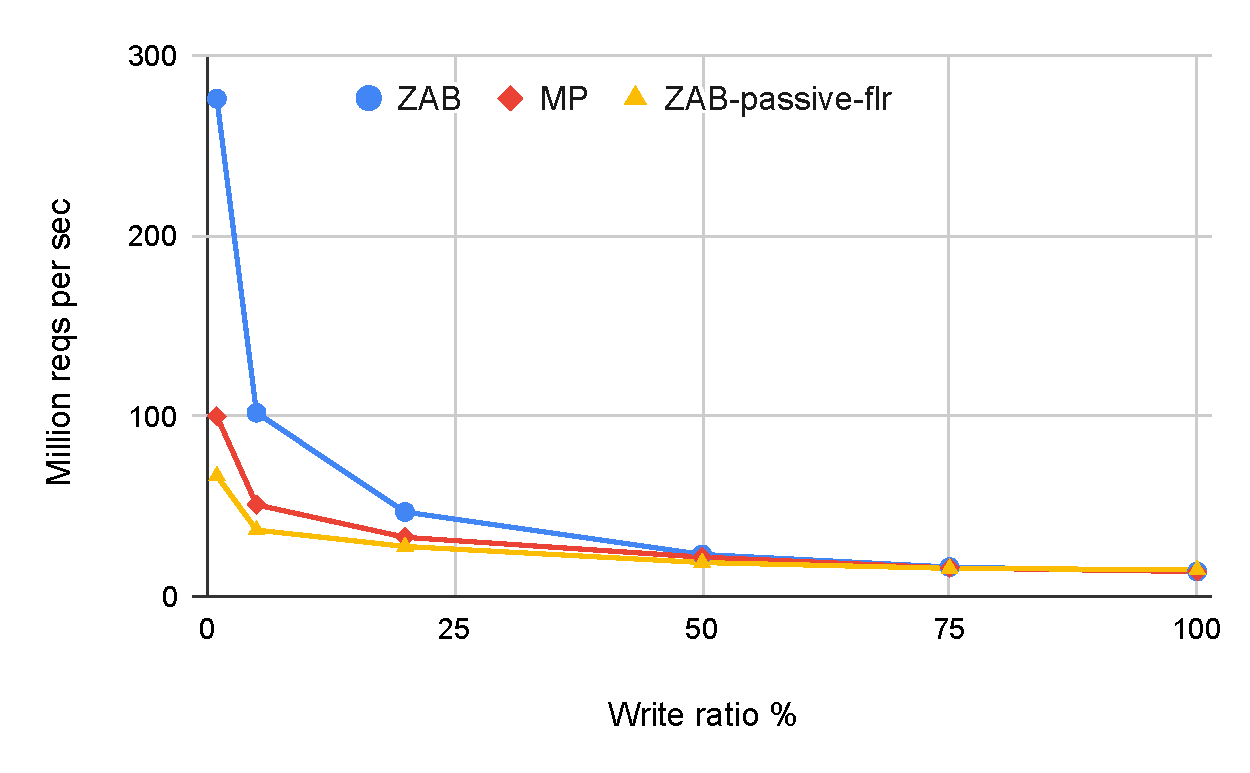
\includegraphics[scale=0.4]{1_figures/zab-passive-flr.pdf}
%   \vspace{-0.5em}
  \caption{Throughput of ZAB, MP and ZAB/MP with passive followers, when varying the write ratio}
%   \vspace{-1.5em}
  \label{fig:zab-psv}
\end{figure}
% \begin{figure}[t]
  \centering
  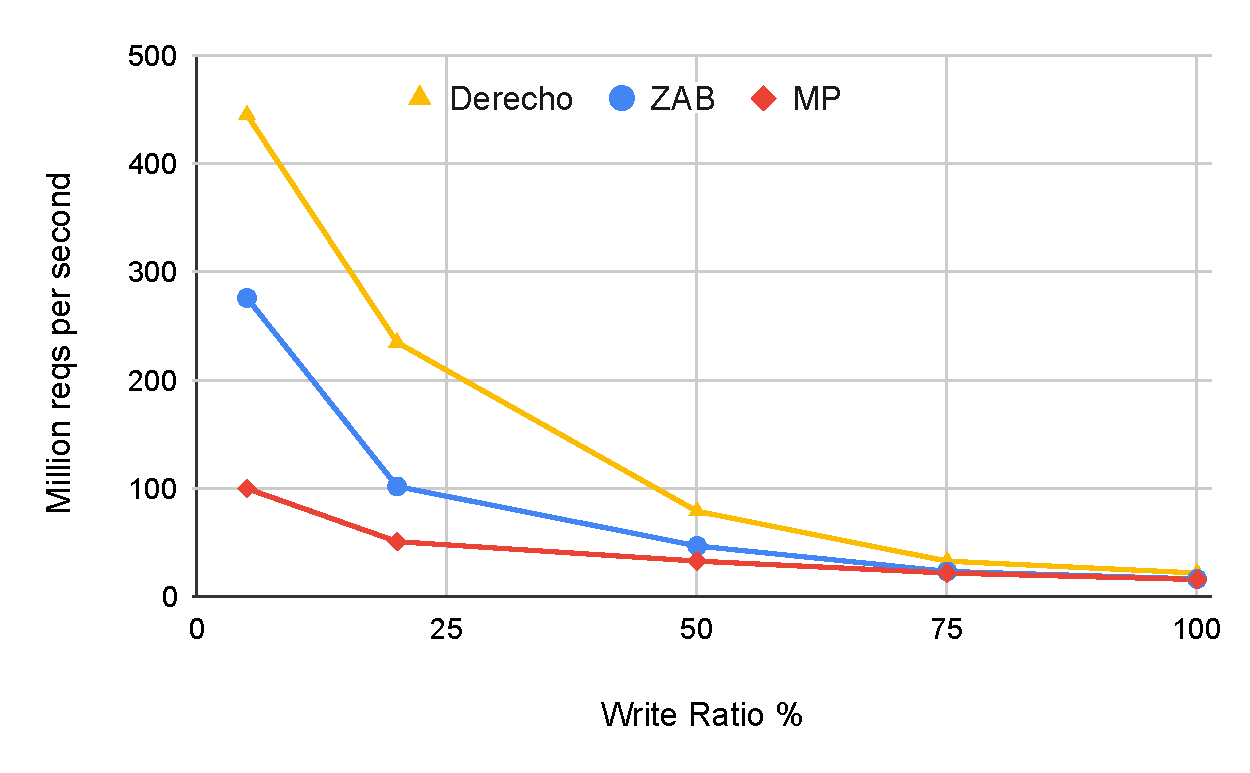
\includegraphics[scale=0.4]{1_figures/zab-mp-dr.pdf}
%   \vspace{-0.5em}
  \caption{Throughput of ZAB, MP \& Derecho, varying the write ratio from 1\% to 100\%}
%   \vspace{-1.5em}
  \label{fig:zab-mp-dr}
\end{figure}
% \begin{figure}[t]
  \centering
  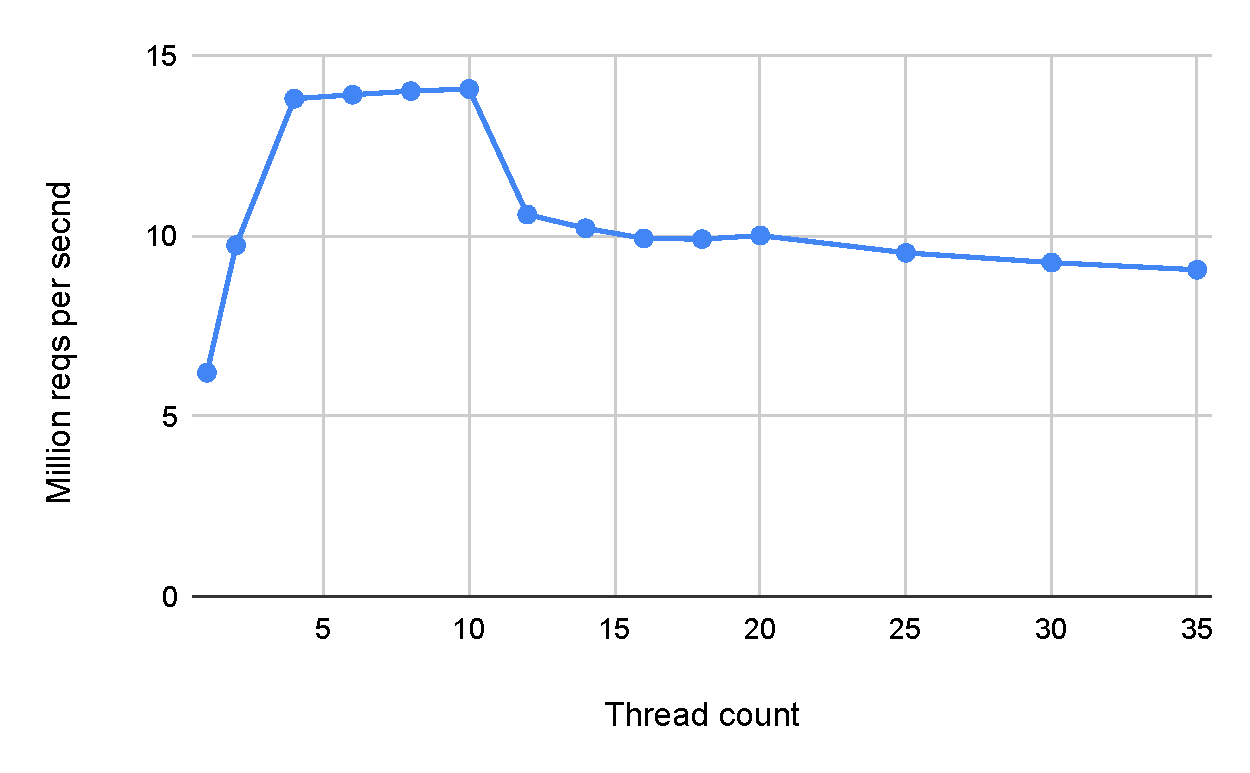
\includegraphics[scale=0.4]{1_figures/ZAB-scal.pdf}
%   \vspace{-0.5em}
  \caption{Write-only throughput of ZAB and MP, varying the workers [5 nodes]}
%   \vspace{-1.5em}
  \label{fig:zab-scal}
\end{figure}
% \begin{figure}[t]
  \centering
  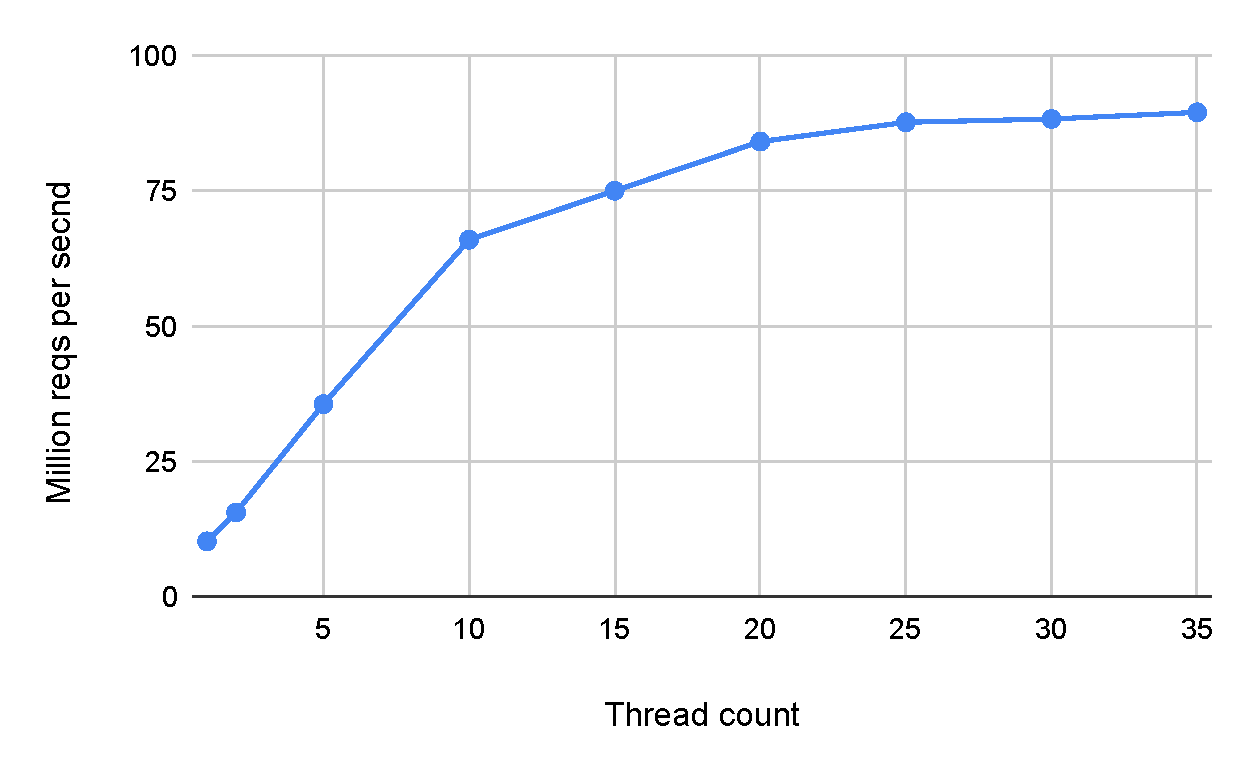
\includegraphics[scale=0.4]{1_figures/Hr-scal.pdf}
%   \vspace{-0.5em}
  \caption{Write-only throughput of Hermes, varying the workers [5 nodes]}
%   \vspace{-1.5em}
  \label{fig:hr-scal}
\end{figure}



\subsection{\DTO: Derecho}\label{sec:ev:dto}
We have already established the effects of the total order in write throughput and contrasted Derecho with ZAB and MP. 
Here we will briefly describe Derecho's operation and comment on its performance in lower write ratios, contrasting it with two \DPKO~protocols.
% Notably our Derecho significantly outperforms the open-source system which performs roughly 250k reqs per second (as evaluated in~\cite{A:2020}) \antonis{Consider downplaying a bit -- e.g., Dereco is a fuller-system(?)}.



\beginbsec{Derecho operation}
In Derecho, writes are totally ordered and applied in that order. The different write-ids are statically pre-allocated to different nodes. Node-0 will propose writes $0$ to $N-1$, node-1 will propose writes $N$ to $2N - 1$, and so on.
Furthermore, Derecho performs reads locally, relaxing the consistency guarantees from lin to SC (similarly to ZAB). 

\begin{comment}
Let us now briefly discuss how we have implemented Derecho.
For each machine we pre-allocate a number of write-ids, in a round-robin fashion. A node's pre-allocated write-ids are again pre-allocated to the workers within it. Therefore, a worker need not synchronize with other workers to discover the next write-id it must use; rather it computes it from its own worker-id and node-id.
Similarly to ZAB, a write requires two broadcast rounds, a prepare and a commit. The receiver of a prepare responds with an ack (implemented with \odlib~ smart-acks). The receiver of a commit, which is also implemented with \odlib~smart-com, need not reply.
Finally, reads are implemented identically to ZAB.
\end{comment}
% \beginbsec{Reads}
\beginbsec{Performance}
Without considering thread-scalability, \DTO\ is a powerful idea as the different nodes need not coordinate in order to serialize the writes. They merely need to compute the order of their own writes through their node-id and broadcast them.
This is why 
Derecho is one of the better performing protocols in single-threaded performance (\figref{fig:single-thr}). 
However, as we saw with ZAB and MP, applying writes in a total order does not scale across many threads.

As discussed in the previous section, Derecho scales better than ZAB at lower write ratios (\figref{fig:zab-mp-dr}); however its low write throughput still limits its total throughput at low write ratios.
%is still limited by its small write throughput.
For instance, when compared with Hermes (lin local reads) and CP (ABD reads) in \figref{fig:hr-dr-cp}, Derecho is significantly outperformed by Hermes even in low write ratios, because Hermes has a higher write throughput (due to its thread-scalability), which allows it to scale well at low write ratios. 
% In contrast, the low write throughput of Derecho, limits its throughput
However, Derecho's local reads allow it to outperform CP, on low write ratios, despite the fact that CP has a higher write throughput.

\begin{figure*}[t]
\centering
  \begin{subfigure}[t]{0.33\textwidth}
    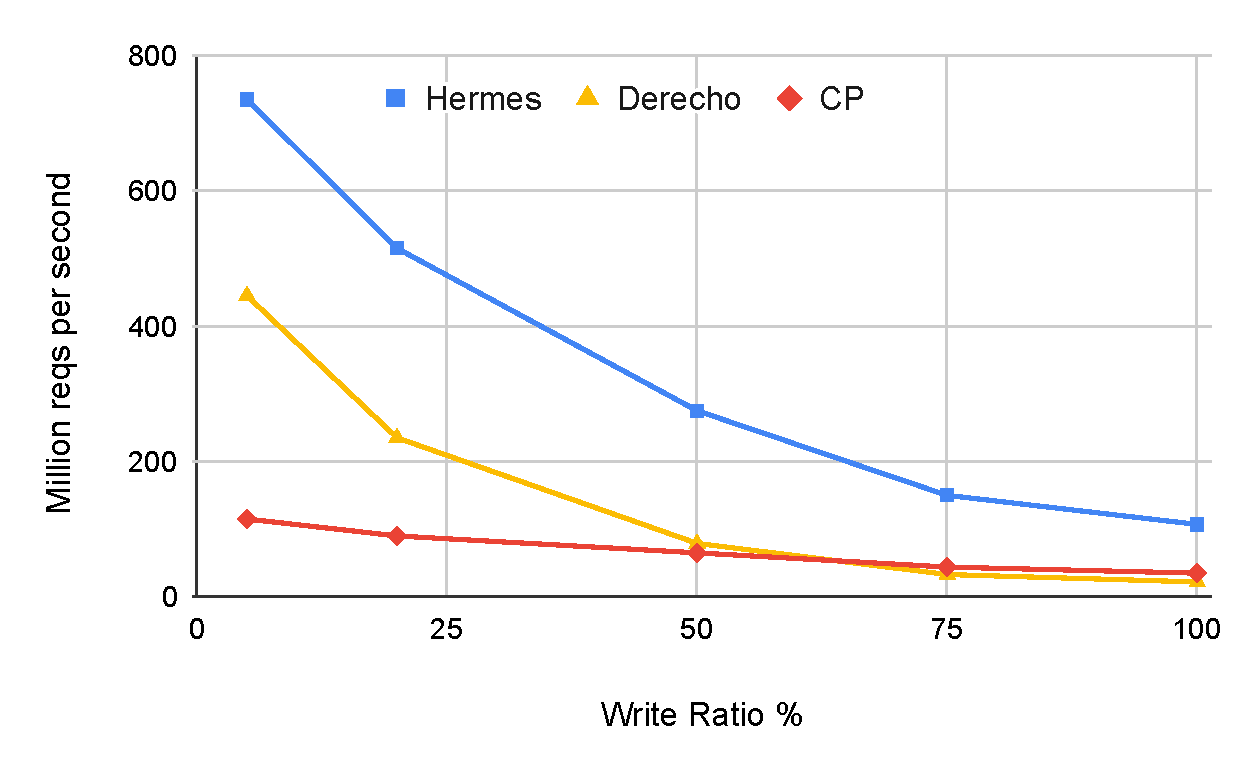
\includegraphics[width=\textwidth]{1_figures/hr-dr-cp.pdf}
    \captionsetup{width=\linewidth}
    % \vspace{-1.8em}
   \caption{Hermes, Derecho \& CP}
%   \vspace{-1.5em}
  \label{fig:hr-dr-cp}
  \end{subfigure}
  %
  \begin{subfigure}[t]{0.33\textwidth}
    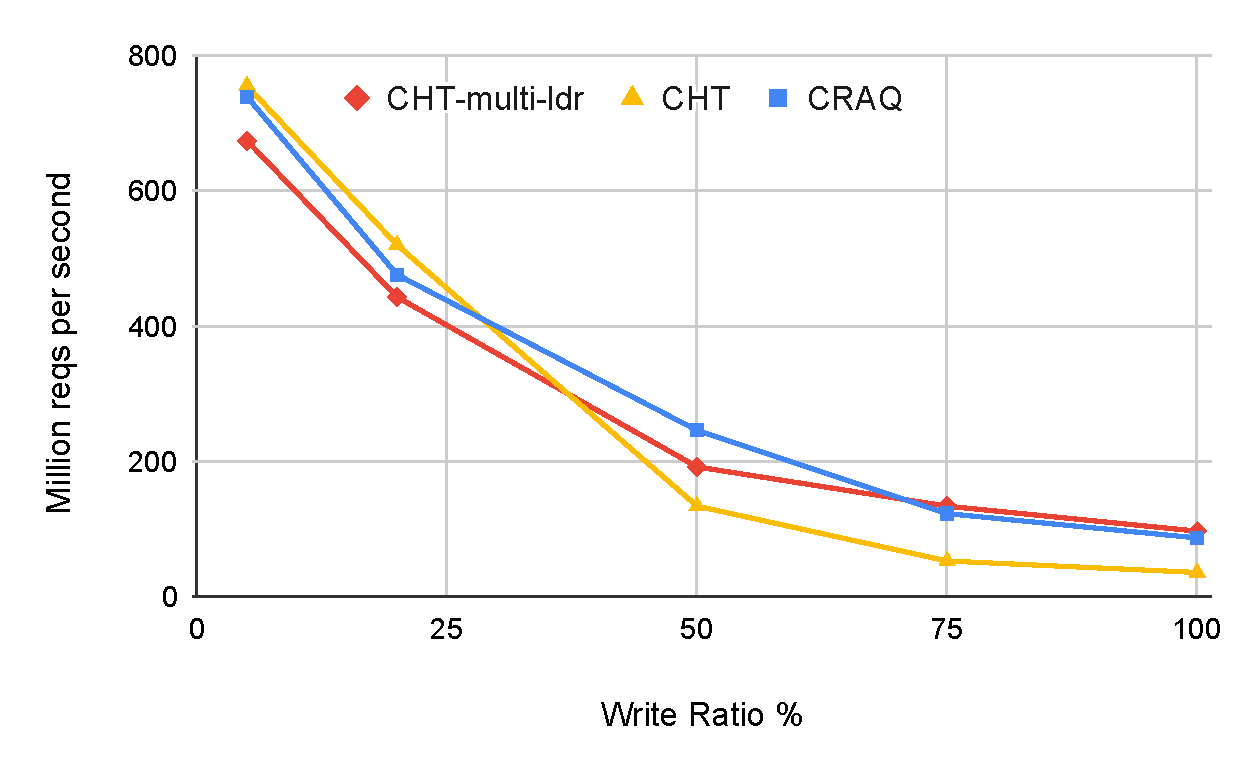
\includegraphics[width=\textwidth]{1_figures/craq-cht-chtml.pdf}
    \captionsetup{width=0.95\linewidth}
    % \vspace{-1.8em}
    \caption{CHT-multi-ldr, CHT \& CRAQ}
%   \vspace{-1.5em}
  \label{fig:cht-cht-craq}
  \end{subfigure}
  %
  \begin{subfigure}[t]{0.33\textwidth} 
  
    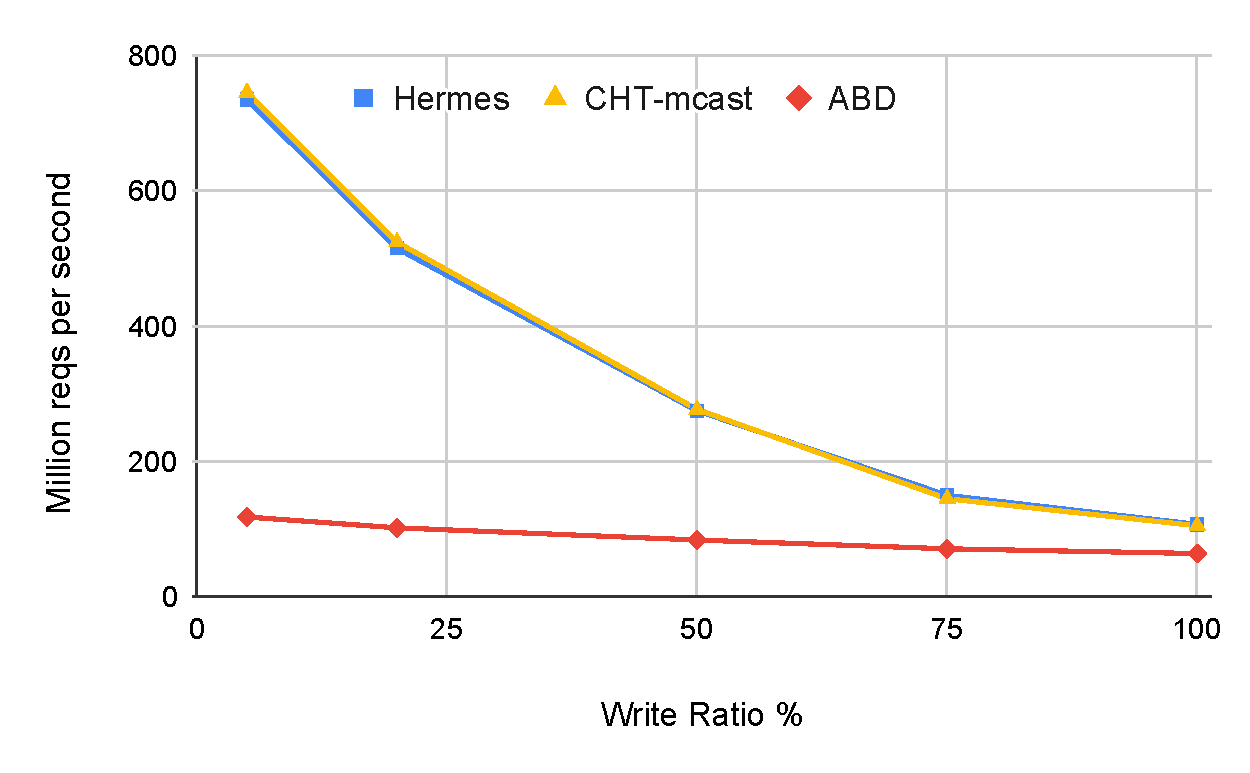
\includegraphics[width=\textwidth]{1_figures/hr-chtm-abd.pdf}
    \captionsetup{width=0.90\linewidth}
    % \vspace{-1.8em}
    \caption{Hermes, CHT-mcast \& ABD}
%   \vspace{-1.5em}
  \label{fig:hr-cht-abd}
  \end{subfigure}
%   \vspace{-1em}
  \caption{Throughput vs. write ratio}
  \label{fig:three-graphs}
%   \vspace{-1em}
\end{figure*}

% \begin{figure}[t]
%   \centering
%   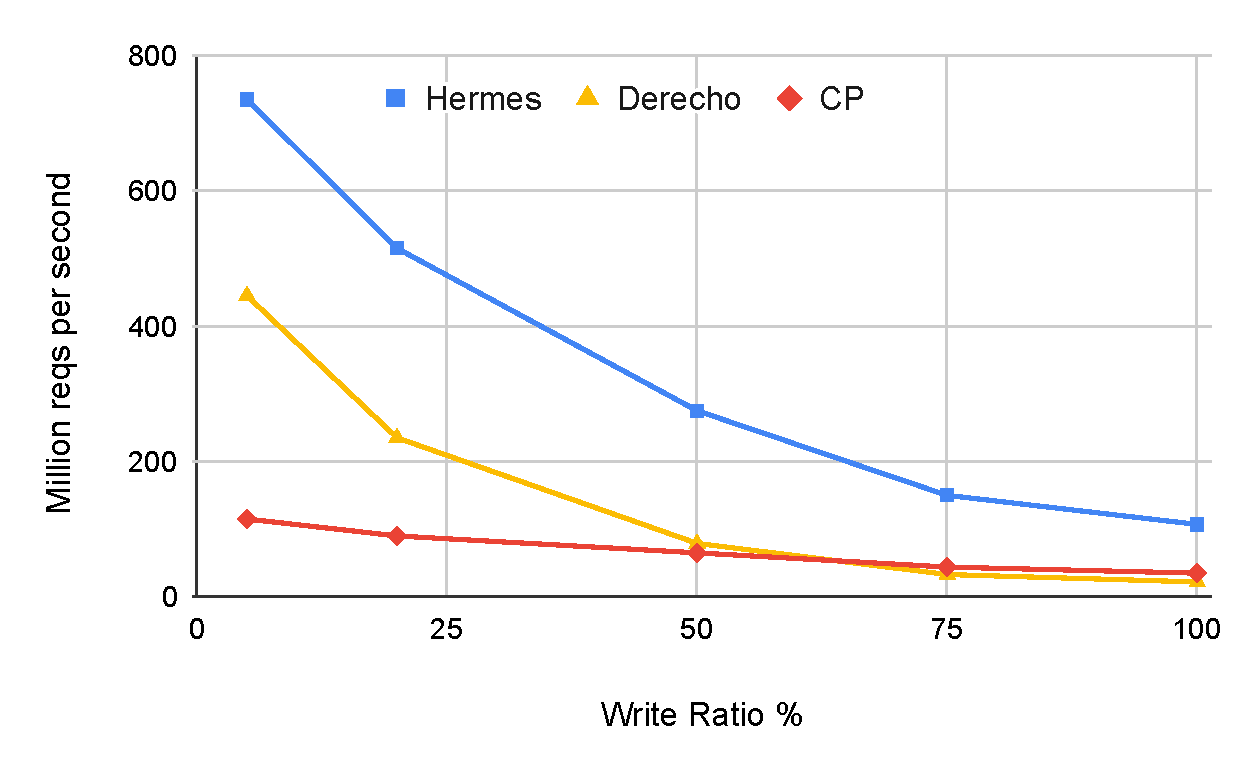
\includegraphics[scale=0.4]{1_figures/hr-dr-cp.pdf}
% %   \vspace{-0.5em}
%   \caption{Throughput of Hermes, Derecho \& CP, varying the write ratio from 1\% to 100\%}
% %   \vspace{-1.5em}
%   \label{fig:hr-dr-cp}
% \end{figure}

\subsection{\LPKO: CHT, CHT-multi-ldr, and CRAQ}\label{sec:ev:lpko}

We start the discussion of the \LPKO~protocols with CHT and then extend it to CRAQ. 

% To the best of our knowledge this is the first implementation of CHT. CHT-multi-ldr is similar to FGSMR~\cite{Liu:2020}, whose performance is significantly lower at a few hundred thousand requests per second. Finally, the throughput of the CRAQ open-source implementation~\cite{Terrace:2009} is a few thousand requests per second.

\beginbsec{CHT operation}
All writes in CHT are propagated to the leader. The leader completes the writes in two broadcast rounds, similarly to ZAB and MP, with two differences: 1) it does not create a total order of all writes and 2) it waits until a write has reached all followers before committing it. 
The latter allows for local reads at the follower nodes. Notably, reads need to block if there is an ongoing write to the same key, until that write commits. %; when the write commits the read can complete. %This blocking is inevitable for lin reads, as proven in the CHT paper~\cite{Chandra:2016}

\begin{comment}
Let us briefly discuss a few implementation details.
Firstly note that reads are subtly different than ZAB and Derecho.
Specifically, because reads are lin, it must be that once a read returns a value, a later read can never return an earlier value. To achieve this, we maintain a state variable with each key, initially denoting that the key is \qt{valid} and can be read. Upon receiving the first round of a write, the state transitions to \qt{invalid}, denoting that the value cannot be read until the write is committed. Reads that find a key in invalid state will be buffered to be retried in the future. Note that this blocking of lin reads is inevitable as proven in the CHT paper~\cite{Chandra:2016}. 

The implementation of writes are again similar to ZAB and MP with a subtle difference.
In order to support multi-threading, we have added a version to each key (as part of its metadata).
The per-key version is incremented by the leader, each time it writes the key. Then the version is sent along with the write in the first broadcast round.
To understand why the version is necessary assume that two different workers of the leader attempt to write the same key concurrently. 
The two writes will serialize at he leader node due to the concurrency control at the KVS: whoever grabs the lock first will also write first.
However, that ordering of the two writes must be honoured in the follower nodes. This will be achieved with the per-key version. Plainly, the version of the later write will be bigger, allowing the followers to serialize the writes in the correct order.
\end{comment}

In CHT-multi-ldr each node is the leader for $1/N$ of all keys, with $N$ being the number of nodes. 
% The partitioning is done by using modulo N on the key.
% Therefore, u
Upon receiving a write request for key $K$, the worker finds out the leader for that key through a simple modulo operation on the key. Then, similarly to CHT, the write is propagated to its leader, which executes it to completion. %In our setup this simple partitioning scheme creates a uniform distribution of keys to leaders.


\beginbsec{CRAQ operation}
CRAQ organizes the nodes in a chain. All writes are steered to the head of the node, which then propagates them down the chain. When a write reaches the tail (\ie the last node of the chain), it is said to be committed and an ack propagates back, all the way to the head. On receiving the ack, nodes commit the write.
% Note the big difference with CHT: the head does not broadcast the write to everyone; instead it only sends it to the next node.
% Consequently, all nodes share in the load of committing a write, except the tail, which only sends back acks.
Reads are executed locally. As an optimization, reads do not block when there is an ongoing write to the same key, but instead are propagated to the tail. The tail is guaranteed to always know the latest committed write, because of its position in the chain. 
%In our setup, this optimization does not yield any performance benefits compared to simply blocking the read until the write is committed.

\begin{comment}
First note the similarities with CHT: writes carry a per-key version, which is decided by the head node and is used to enforce keys are serialized correctly in all nodes.
In addition, in order to support lin reads, writes change the state of keys to \qt{invalid}. When the write is acked  the state changes back to \qt{valid}.

Now note a few important differences with CHT. 
Firstly, there is no commit messages, messages simply commit when the ack (smart-ack that is) is propagated to them from the tail. Notably the tail has a special role: it immediately commits all writes when receiving them, and thus it never transitions its keys to \qt{invalid} state. As such the tail always knows the latest committed value for each key.
As an optimization, reads in non-tail nodes that find the key in \qt{invalid state} are propagated to the tail, instead of being buffered and retried (as in CHT). We implement these as smart-reads: if the tail holds the same version it will answer with a 1-byte opcode. We have found that this optimization does not make a difference compared to the simpler act of buffering, but still use it in our measurements.
Finally, note the big difference maker with respect to CHT: the head does not broadcast the write to everyone; instead it only sends it to the next node.
Consequently, all nodes share in the load of committing a write, except the tail, which only sends back acks.
\end{comment}

\beginbsec{Performance}
Firstly, recall that from \figref{fig:write-all}, we observed that CHT cannot balance the load and is bottlenecked by the send side of the leader, which saturates its NIC. There are three possible optimizations: using multiple leaders (CHT-multi-ldr), using a chain (CRAQ), and finally using the hardware multicast primitive (CTH-mcast). 

Notably, CRAQ has the lowest impact among the three techniques,
%CHT-mcast performs better than CHT-mulit-ldr which in turn performs better than CRAQ. 
% This is 
because it does not completely balance the load, as the tail does not contribute in the propagation of a write. In our 5-node deployment, the load is split between 4 nodes which explains why CRAQ reaches only 4/5 of the throughput of a well-balanced protocol such as CHT-mcast.

CHT-multi-ldr also falls short of CHT-mcast. The reason is a bit subtler. There is less opportunity to amortize cpu and network costs in CHT-multi-ldr, because writes need to be steered to different leaders. 
% has to be both follower and leader, it must propagate writes to the different leaders it cannot find the same opportunity to amortize cpu and network costs.
For example, assume that in our 5-node deployment a worker in one of the nodes receives 5 write requests from a client. Also assume that each request must be steered to a different leader. The worker cannot batch all messages to the same packet. Instead, it must create a packet for each of the writes, sending them to the different leaders. Furthermore the worker itself may be the leader for one of the writes, which means it must broadcast it, again losing the opportunity to batch it with other writes. 
Conversely, in vanilla CHT, the worker would simply batch all writes to the leader.

% The third optimization is exemplified by CHT-mcast, which enhances CHT with the multicast primitive.
CHT-mcast enhances CHT with the multicast primitive.
In CHT, the send side of the leader is overloaded, because the leader broadcasts all writes, and every broadcast requires N unicasts (for N followers). However, the followers receive only one message from each broadcast, and thus when the leader utilizes $100$\% of its send bandwidth, the followers only utilize  $100/N$\% of their receive bandwidth.

CHT-mcast improves upon CHT exactly because in CHT the followers underutilize their receive side.
When the multicast primitive is used, the leader sends one message per broadcast instead of N. The preexisting underutilization in the followers' side allows us to leverage the leeway created by the multicast at the leader's send side, to send more writes to the followers.
Had there been no room in the receive side of the followers, the multicast would simply reduce the bandwidth used at the leader send side, without improving performance.
In fact this is exactly what happens for most of the broadcasting protocols (ABD, Hermes, CHT-multi-ldr, Derecho).
Notably, ZAB and MP, even though leader-based, are not scalable enough to tap into the multicasts benefits. %  enough to profit from multicast.
%would be useful for ZAB and MP, if they were scalable enough to saturate the send side of the leader.
% This also explains why the rest of the protocols do not see significant improvement when using the multicast: there is no preexisting room in the receive side of nodes to allow broadcasters to send more messages.
% Notably, in the case of the non-thread-salable protocols (\eg ZAB), multicast is not useful because the bottleneck is not at the network side.

% CHT-mcast improves upon CHT because in CHT the follower's receive side is underutilized. This allows us to leverage the leeway created by the multicast at the leader's send side by sending more packets to the followers. Had the follower's receive side not been underutilized, the multicast would simply reduce the utilization of the leader's send side.

% The multicast primitive offloads the send side of the leader, taking advantage of the fact that the receive side of the follower 


\figref{fig:cht-cht-craq} shows the throughput of CHT-multi-ldr, CHT and CRAQ when varying the write ratio. Firstly note that CHT outperforms the other two for low write ratios.
This is because 1) CHT has a smaller work-per-request ratio and 2)~CHT is not bottlenecked by the leader's send side at low write ratios.
CHT's work-per-request ratio is smaller than CRAQs, because broadcasting writes is more efficient than propagating them through a chain, as it allows for a better amortization of compute and network costs.
CHT-multi-ldr has an even higher work-per-request ratio than CRAQ, because 
as the write ratio decreases, the opportunity to amortize costs by batching writes reduces, exacerbating its pre-existing problem. %, increasing its work-per-request ratio.
This is why it is outperformed by both CRAQ and CHT.
% because of its simplicity.
% However, as the write ratio increases, CHT becomes bottlenecked by the leader's send bandwidth, at lower write ratios.
CHT-mcast scales CHT's throughput at high write ratios as it avoids the bottleneck in the leader's send side bandwidth.
As a result, its throughput is at the highest level for all write ratios, matching that of Hermes (\figref{fig:hr-cht-abd}).
%is the highest from all \pnum~protocols matching that of Hermes,
%matches that of Hermes (\figref{fig:hr-cht-abd}), which is the best performing protocol.

% is enhanced with the multicast primitive, the bottleneck is removed, and its performance matches that of Hermes
% For CHT-multi-ldr, as the write ratio decreases, the opportunity to amortize costs by batching writes becomes increasingly harder, which is why it is outperformed by both CRAQ and CHT.




\subsection{\DPKO: CP, All-aboard, ABD, and Hermes}\label{sec:ev:dpko}

Firstly we briefly explain the operation of the protocols and then discuss their performance.

 
\beginbsec{Operation}
In \DPKO~protocols, each node coordinates its own writes.
An ABD write requires two broadcast rounds. The first round finds out the version of the key stored in a majority of nodes and the second sends out the new value.
An ABD read requires one broadcast round with an optional second. The first round finds out the latest value from a majority of nodes. If the reader cannot infer from the replies to its first round that a majority of nodes store this value, then it performs a second round to broadcast it. Notably, the second round is not necessary in more than 99\% of the reads.

CP requires three broadcast rounds to complete a write: propose, accept and commit.
All-aboard is an optimization over CP, allowing a write to commit after two rounds when there are no conflicts or slow nodes, using CP as a fallback.
%in case of a conflict. However, if an accept cannot gather a positive ack from all remote nodes, then CP is executed. 
% In our setting, All-aboard is successful in more than 99\% of writes.
Both CP and All-aboard execute reads using ABD reads.
%~\antonis{Q: Does this work in the case of conflicts/overlaps with concurrent writes(?)}.
Finally, Hermes requires two broadcast rounds to complete a write. Its rounds are substantially more light-weight than CP and All-aboard (and even ABD) but all messages must always reach all nodes. For that reason, Hermes reads are local.



\begin{figure}[t]
  \centering
  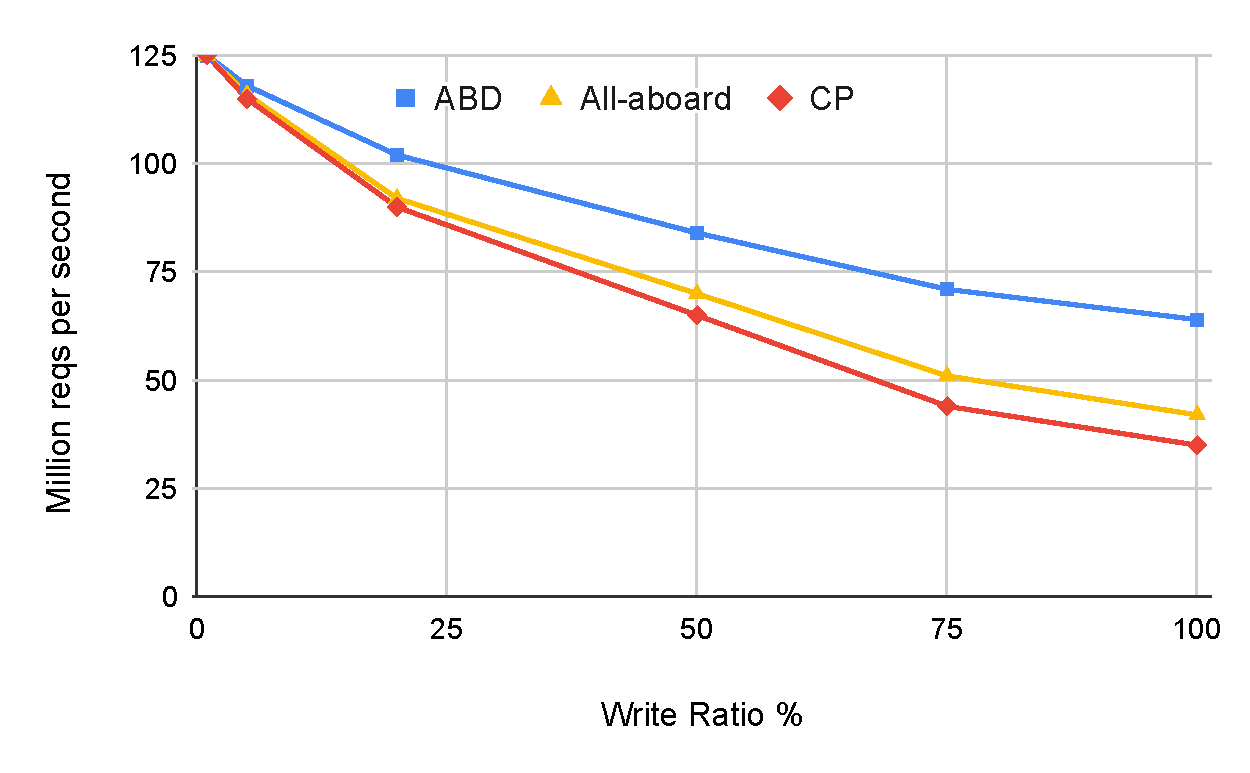
\includegraphics[width=0.4\textwidth]{1_figures/abd-ab-cp.pdf}
%   \vspace{-1.5em}
  \caption{Throughput vs write ratio for ABD, All-aboard \& CP}
%   \vspace{-1.5em}
  \label{fig:abd-ab-cp}
\end{figure}

\beginbsec{Performance}
Firstly, from \figref{fig:single-thr}, we observe that CP has the lowest single-threaded performance. This is because of the extremely high work-per-request ratio required in CP, as explained in \secref{sec:tax:dpko}. However,  CP is thread-scalable and well load balanced, enjoying a 10x improvement when multi-threaded (\figref{fig:write-all}) outperforming ZAB, MP and Derecho and matching CHT.

The All-aboard optimization reduces CP's high work-per-request but not completely.
This is why All-aboard is the second worse protocol when single-threaded.
Note that All-aboard has a significantly higher work-per-request ratio than Hermes and ABD, which also require two broadcast rounds. 
This highlights the fact that simply using the number of broadcast rounds as a metric to gauge performance is not sufficient. We need to factor in the size of the messages and the responses along with the complexity to create them.


Similarly to CP, All-aboard scales very well (10x) when multi-threaded, outperforming CP, CHT and the total order protocols.
Recall from \secref{sec:fail} that CP and All-aboard are the only two protocols (out of the \pnum) that can perform conditional writes while remaining available in the event of a failure. Therefore, for those keen on offering high availability, All-aboard comprises a great candidate, as it can also provide reasonably high performance.


ABD also offers the same levels of availability, but it is the only protocol out of the \pnum~that cannot perform conditional writes.
This simplification affords ABD a significantly lower work-per-request ratio than CP and All-aboard, which is why ABD outperforms CP and All-aboard both single-threaded and multi-threaded.
\figref{fig:abd-ab-cp} compares ABD, CP and All-aboard, varying the write ratio. Notably the read throughput is equal for all three, as they all implement ABD-reads. However, as the write ratio increases, ABD outperforms the other two due to its lower work-per-request ratio for writes.
Therefore, ABD comprises a great candidate, in cases where high availability is required and simple writes will suffice (as opposed to conditional writes).

\figref{fig:hr-cht-abd} compares ABD with Hermes (and CHT-mcast). Even though ABD is within a close distance in the write throughput, there is a big gap in the read throughput, demonstrating the cost of high availability. Specifically, Hermes mandates that every write reaches every node. In doing so, it concedes that all nodes must block on a failure (discussed in \secref{sec:fail}). However, it takes advantage of this concession in both reads and writes. In reads, by enabling them to execute locally, leveraging that all nodes have received the latest committed write. And in writes, by accelerating their operation, leveraging that a node that performs a write, has received all concurrent, conflicting writes.

This renders Hermes the better performing protocol out of all \pnum, making it an ideal candidate, for those who can afford an unavailability period in case of a failure.




\begin{comment}
\subsection{Hardware Multicast}\label{sec:ev:mcast}
Here we will discuss why the multicast primitive provides a 3x benefit for CHT, but no more than 5\% for the rest of the protocols.
The reason is that the multicast only relieves the send side of a broadcast.
% Using the hardware multicast primitive provides a 3x benefit for CHT. The benefit for the rest of the protocols is very small, typically around 5\%.
Specifically, on a multicast, one packet is sent to the switch instead of N (assuming N receipients). The switch then replicates the packet N times, propagating it to all recipients. Without using the multicast primitive, the sender must send N packets.
Let us use \figref{fig:mcast}, to investigate how multicasting affects CHT and Hermes.

\figref{fig:mcast} provides a pictorial view of the usage of the send and receive bandwidth for CHT, CHT-mcast, Hermes and Hermes-mcast. Firstly note that the figure does not provide a precise view of the measurements. Rather it illustrates a rough approximation that will help us explain why multicast is helpful in certain scenarios. To simplify further, in this discussion we will assume that smart-acks and smart-commits consume zero-bandwidth.

In \figref{fig:mcast}a, we see that the CHT leader uses up all of its send bandwidth. The leader utilizes a small fraction of its receive bandwidth receiving followers' writes.
% that are steered to it from the followers.
The receive side of the follower is not well utilized, because it only receives $1 / N$ of the messages sent by the leader (assuming an N-side deployment). The send side of the follower is used only to propagate writes to the leader. 

In \figref{fig:mcast}b we see how CHT is affected when using the multicast.
Leader's send side is still saturated, but now each packet is only sent once. Therefore, now the leader sends N times as many distinct packets.
Each follower now receives all the packets that the leader sends, because each packet is getting replicated at the switch and sent to all followers. Thus the follower's receive bandwidth is also saturated. Note that the send side of the follower is also increased, as the follower now propagates more packets to the leader. For that reason, the leader's receive side is saturated too.

Note the key insight: CHT-mcast improves upon CHT because in CHT the follower's receive side is underutilized. This allows us to leverage the leeway created by the multicast at the leader's send side by sending more packets to the followers. Had the follower's receive side not been underutilized, the multicast would simply reduce the utilization of the leader's send side.

This is exactly what happens with Hermes and Hermes-mcast in \figref{fig:mcast}c and d. In Hermes, all nodes utilize both the send and receive bandwidth symmetrically. Therefore, when multicast
is employed, the leeway created at the send side cannot be leveraged, because no node can receive any more packets.

To understand why CHT-mcast can match the performance of Hermes (or Hermes-mcast), consider the send bandwidth of the leader of CHT-mcast and the send bandwidth of a node in Hermes-mcast. Specifically, each Hermes-mcast node receives multicasts from the rest $N-1$ nodes. Therefore, each node can use up to $1/N-1$ of its send bandwidth. 
Therefore, all $N$ Hermes-mcast nodes use $N/N-1$ of one node's send bandwidth to multicast new writes.
Comparing that with CHT-mcast, we can infer that Hermes-mcast can in theory be only $N/N-1$ times better than CHT-mcast. For instance in our 5-node deployment, Hermes should be able to achieve a 25\% increase over CHT-mcast. 
Furthermore, in theory Hermes and Hermes-mcast should have the same performance.

\figref{fig:hr-cht-abd}, shows that in practice, because Hermes does not manage to fully saturate its send bandwidth, CHT-mcast and Hermes (without multicast) have almost identical behaviour for all write ratios. Finally, the write throughput of Hermes-mcast (94 M.reqs/s) is around 10\% better than CHT-mcast.


\begin{figure}[t]
  \centering
  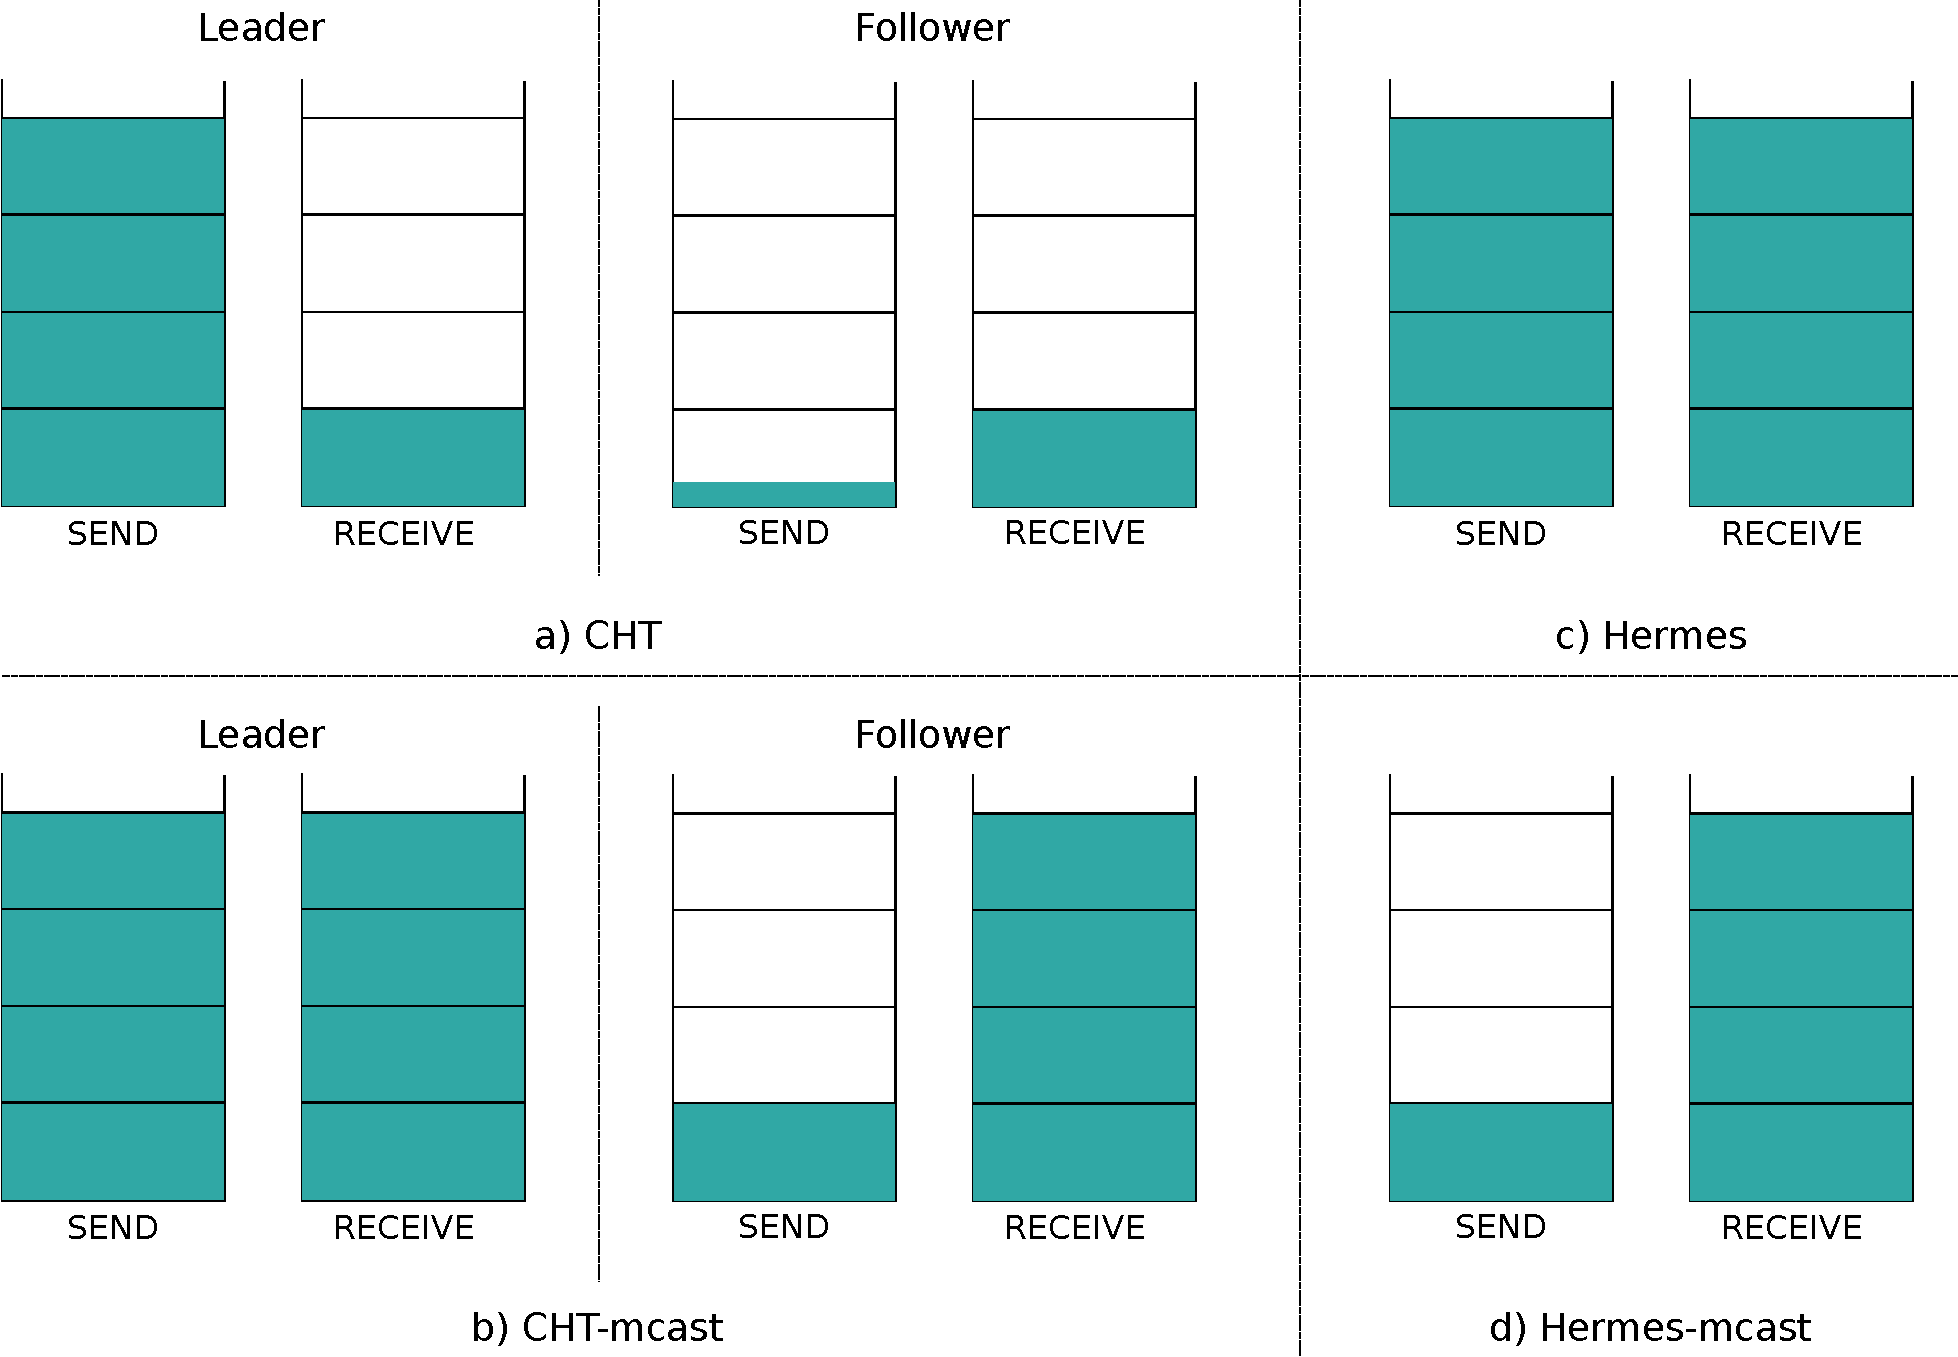
\includegraphics[width=0.47\textwidth]{1_figures/mcast.pdf}
%   \vspace{-0.5em}
  \caption{An illustration of the send and receive bandwidth of CHT, CHT-mcast, Hermes and Hermes-mcast}
%   \vspace{-1.5em}
  \label{fig:mcast}
\end{figure}
% Therefore, in a load balanced scenario, where each machine sends out as much data as it receives, using the multicast will not help even if the bottleneck is at the network. Because the pressure is relieved \emph{only} on the send side. The nodes will keep receiving the same amount of packets.

% In CHT's case, for each write the leader must do a broadcast, \ie  send N-1 unicasts.
% In return it only receives small smart-acks. 
% The followers only receive one message per write.
% Therefore the send side of the leader is substantially more loaded. As a result, CHT scales only up to five threads (\ie workers), which are enough to saturate the leader's send side of our 56 Gbit NIC. Beyond that the write throughput flatlines at 28 M.reqs/s.

% When enabling multicast, the leader's send side gets relieved and the throughput scales up to 85 M.reqs/s. Note however, that CHT-mcast still does not utilize all available resources: followers' send side are still underutilized. How does it then match Hermes' performance?
% CHT-mcast sends one message per write where Hermes sends N-1 (with N nodes). And thus Hermes needs to utilize all nodes' send bandwidth, to provide the same throughput. However, Hermes cannot utilize the multicast: even when it uses it the send side of all nodes get relieved but the receive side remains jammed.



% only needs to send one message per write.
% The followers each receive one message. The protocol still does not utilize all available resources: leader's receive side and followers' send side are still underutilized. How can then CHT-mcast match Hermes, which uses all resources?

% Compare that to Hermes, where each write 


%  This is why in our results we only use multicast for CHT.
\end{comment}
\begin{comment}
\beginbsec{Writes}
ABD assumes that each object is stored along with a unique identifier of its last write. Most commonly that is a Lamport logical clock~\cite{Lamport:1978}.
We will refer to that unique identifier as timestamp (TS).
A write to key $K$ requires two broadcast rounds. 
A first lightweight round learns the TSes stored in a majority of remote nodes. The writer uses the remote TSes, to create a new larger TS and tag its write, which it broadcasts in its second round.
The write can commit upon receiving a majority of acks (implemented with \odlib~smart-acks).
% The first round requests remote nodes to tell it their locally stored TS for $K$. The writer waits only for a majority of responses (including its own). By the end of the round, the writer knows what is the latest write (by its TS) that has been committed in a majority of replicas. This is because, any write that has been applied to a majority of replicas, must overlap with he majority of responses that the writer received.

\beginbsec{Reads}
Reads perform one broadcast round and then an optional second round.
The first round broadcasts the locally stored TS and asks remote nodes if they store the same TS, a lower one or a higher. If replicas store a higher TS, they respond with both the TS and the value. The read gathers a majority of replies.
If the read cannot infer that a majority of replicas stores the value that the read wishes to return, then it performs a second round, which is identical to the write's second round. The second round is not necessary in more than 99\% of the reads.
\end{comment}
\begin{comment}
Notably, CP has not been widely used to perform conditional writes. This is because in Lamport's original paper it was not described how to run CP repeatedly, but we must be able to modify the same object multiple times. Rather Lamport suggested that CP can be executed once to establish a leader which can then make all decisions (\ie Multi-Paxos).

However, Lamport in his original paper did explain that it is possible to run CP without a log over a KVS. Recently, there have been a few proposals~\cite{Skrzypczak:2020, Rystsov:2018} that combine this observation with enhancements to CP so that it can run repeatedly in order to support conditional writes. 
In fact, Gavrielatos \etal~\cite{V:2020} showed that CP can be competitive, if multi-threaded, however they never revealed any details on how it can be so.

In this work, we replicate the results of~\cite{V:2020}, over \odlib~and we enhance it with  the All-Aboard optimization, sketched in Howard's thesis~\cite{Howard:2019}. % 2) the carstamps proposed by Burke \etal~\cite{Burke:2020}, so that it can be combined with ABD reads and writes.
Notably, the specification of the enhancements required for CP (to run it  repeatedly) and All-aboard are out of the scope of this paper. However, as a companion to this paper, we will also publish the full specification and implementation description of both our CP and All-aboard. 
%The specification safely extends CP so that it can be executed repeatedly, and it elaborates on multi-threading CP.
Below we provide a brief description of the implementation of writes in CP and All-aboard.

\beginbsec{Writes}
CP requires three broadcast rounds to complete a write: propose, accept and commit. Upon receiving any of the three messages, a worker locks the corresponding key-value pair, it examines its CP-related metadata (\eg its timestamps), it modifies it accordingly and it replies. 
Proposes and accepts can be acknowledged (acked) or negatively-acked (nacked).
Commits require no response.
Upon receiving a majority of acks for a propose, the worker, that coordinates the write, broadcasts accepts. Upon a majority of acks to an accept the write can be committed. 

All-aboard omits the first round (proposes) and directly broadcasts accepts.
If \emph{all} remote nodes ack the accept, then the write can be committed, and commits are broadcast. If the accept does not manage to gather all acks, either because of a nack or because of a slow node, then it starts over running full CP. In our setting, All-aboard is successful in more than 99\% of writes.

% \beginbsec{Reads}
% We implement reads through a modified version of ABD reads. ABD reads require one broadcast round with an optional second. ABD assumes each key is stored along with its The first round broadcastsasks remote nodes if they are storing the same version , the first to read the version of the key from a majority of nodes.


\subsubsection{Performance}
% \begin{figure}[t]
  \centering
  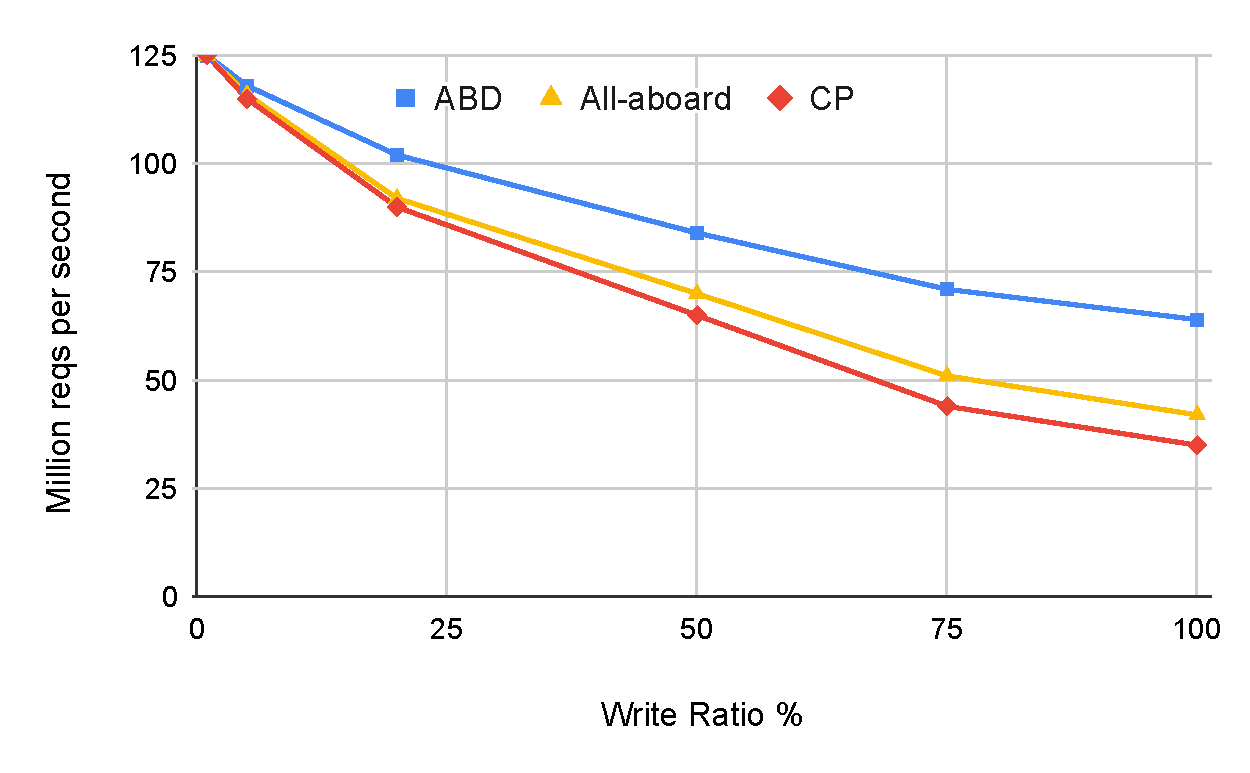
\includegraphics[width=0.4\textwidth]{1_figures/abd-ab-cp.pdf}
%   \vspace{-1.5em}
  \caption{Throughput vs write ratio for ABD, All-aboard \& CP}
%   \vspace{-1.5em}
  \label{fig:abd-ab-cp}
\end{figure}
% \begin{figure}[t]
  \centering
  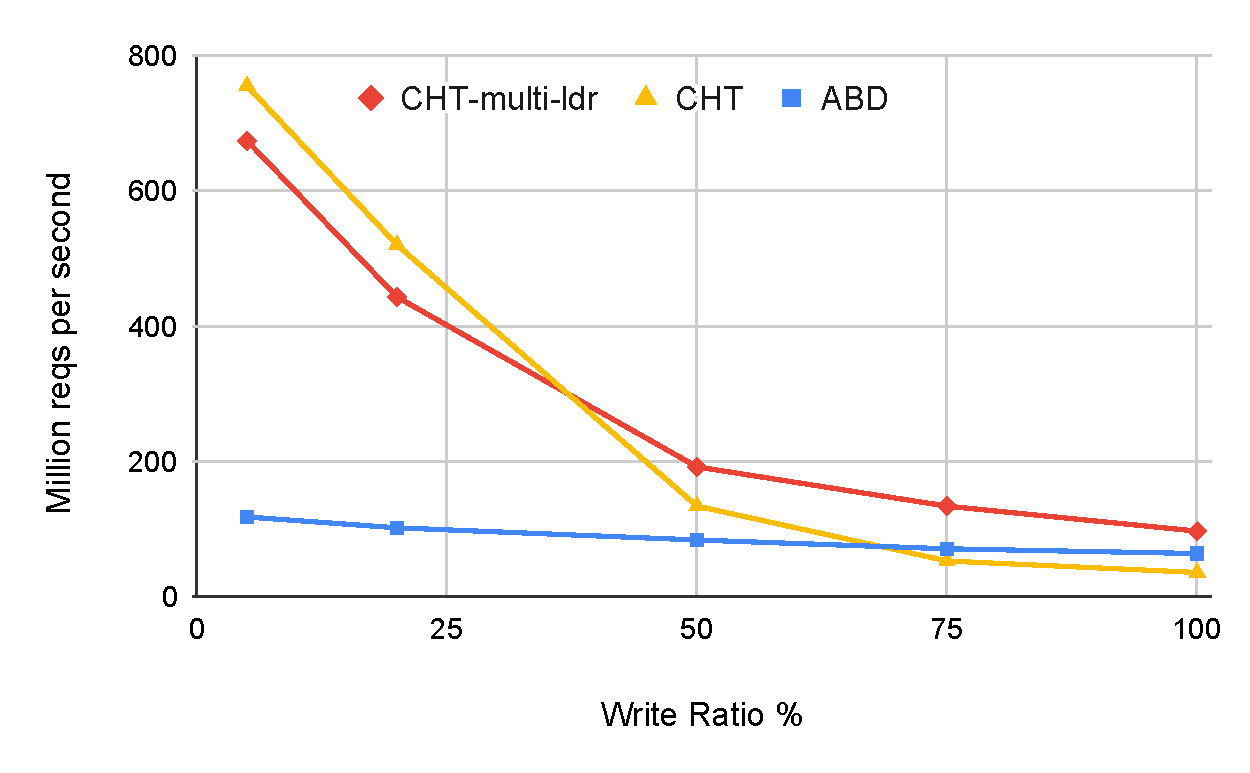
\includegraphics[scale=0.4]{1_figures/chtml-cht-abd.pdf}
%   \vspace{-0.5em}
  \caption{Throughput of CHT-multi-ldr, CHT \& ABD, varying the write ratio from 1\% to 100\%}
%   \vspace{-1.5em}
  \label{fig:cht-cht-abd}
\end{figure}
Firstly, from Figures~\ref{fig:write-all} and \ref{fig:single-thr}, we can see that all three protocols scale reasonably well with more threads. 
%And all three are load balanced as all nodes coordinate their own writes.
In fact, CP and All-aboard are the worst performing protocols when single-threaded.
This is because both protocols must do a lot of work to complete a request.
Notably, CP and All-aboard provide a unique design point as the only protocols that can execute a conditional write and remain available in the event of the fault. 
This is the equivalent of asynchronous consensus.
The cost of this is the very high work-per-request ratio.
All-aboard is very attractive design point for a scenario, where 1) availability is the most important concern 2) conditional writes are required and 3) multi-threading is possible.
If simple writes will do, then ABD is the best option.
% For instance the second round of ABD is 48 bytes, while an accept of CP or All-aboard is 76B.

\figref{fig:abd-ab-cp} shows the throughput of ABD, CP and All-aboard. 
ABD cannot solve consensus, but is significantly simpler than CP and All-aboard, which allows it to perform much better in high write ratios.% both when single-threaded and multi-threaded.
However, in low write ratios it's still outperformed when compared with protocols with local reads that are willing to trade-off availability guarantees for performance.
\figref{fig:cht-cht-abd} depicts just that comparing ABD For instance, with CHT and CHT-multi-ldr, both of which perform reads locally.
% Their read-only throughput is the same, as they all use ABD reads.
% Note that even though ABD and All-aboard both require 2 broadcast rounds for their writes, ABD significantly outperforms All-aboard for high write ratios.
% The reason is that the ABD protocol is substantially simpler and the messages are much smaller. For instance, the second round of ABD is 48 bytes, while an accept is 76B. This is the cost of conditional writes, which All-aboard can execute, but ABD cannot.

% Furthermore, all three protocols are significantly outperformed in low write ratios by protocols that can offer local reads. This is depicted in \figref{fig:hr-dr-cp}, where CP is compared to Hermes and Derecho.
% The reads are implemented identically in all three protocols (with ABD reads). In addition, these are the only three protocols 
% A nack to a propose or accept always includes the reason why can have a variety of dif
\end{comment}
\begin{comment}


\subsubsection{Writes}
\figref{fig:write-all} shows the throughput of all protocols in million requests per second (M.reqs/s) for a write-only setting. Firstly, note that there is a protocol called CHT-mcast. This is the CHT protocol (not CHT-multi-ldr), when the hardware multicast is enabled. Secondly note that that all protocols except ABD, can implement conditional writes (\ie RMWs).


Based on \figref{fig:write-all}, we group protocols into low and high-performers and provide a brief explanation in order to relate them.

\beginbsec{Low-performers}
 ZAB, Multi-Paxos and Derecho are the worst performers. The reason is they lack thread scalability, due to the fact that they must create an order among all writes.
Classic Paxos and its optimization All-aboard Paxos are performing better but still suffer from a very high work-per-request index that is fundamental to their internal complexity.
CHT is thread scalable and has a relatively low work-per-request ratio but does not manage to balance the load: it is bottlenecked by the send bandwidth of the single leader.

\beginbsec{High-performers}
All of the high-performers are mostly thread scalable, load balanced and with a low work-per-request. Hermes serves here as the baseline, as it is completely load balanced, perfectly thread-scalable and has the lowest work-per-request.  
ABD, CHT-multi-leader and CHT-mcast have a bit higher work-per-request than the rest. ABD in order to ensure perfect availability and CHT-multi-leader and CHT-mcast in order to steer writes to the leader.
Finally, CRAQ is not perfectly load balanced as the tail node does not equally participate in the load.  

\subsubsection{Reads}
\figref{fig:write-5per} shows the throughput in M.reqs/s for a read-mostly workload (5\% writes).
First note that both the x-axis and the y-axis are different from \figref{fig:write-all}.
Secondly, note that ZAB and Derecho offer Sequential Consistency, while the rest offer Linearizability. As before, ABD writes cannot be conditional (\ie RMWs).

Operationally there are three groups. Multi-Paxos steers reads to the leader node.  CP, All-aboard and ABD use ABD reads. The rest all use local reads. 

Multi-Paxos performance suffers as its the only non-thread-scalable protocol that does not perform reads locally.  
CP, All-aboard and ABD all come close to the maximum ABD-read throughput (125 M.reqs/s). 

% two issues: firstly the work-per-request is the highest among all protocols we evaluate. This however is balanced with the high availability they offer. Both protocols can continue operating without interruption in the face of a failure. The other problem is that CP and ABP are not perfectly thread-scalable. Because of the 

% \begin{figure}[t]
  \centering
  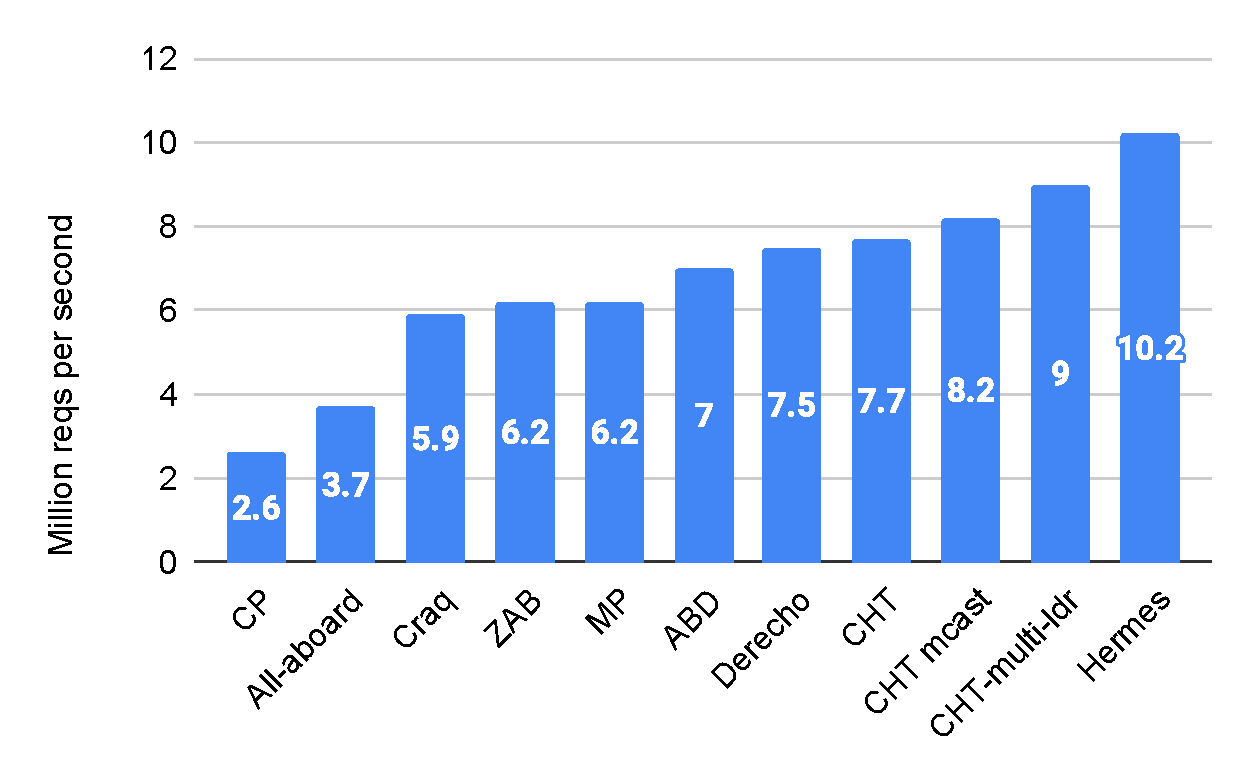
\includegraphics[scale=0.4]{1_figures/single-thread.pdf}
%   \vspace{-0.5em}
  \caption{Single-threaded write throughput of all protocols}
%   \vspace{-1.5em}
  \label{fig:single-thr}
\end{figure}
% \begin{figure}[t]
  \centering
  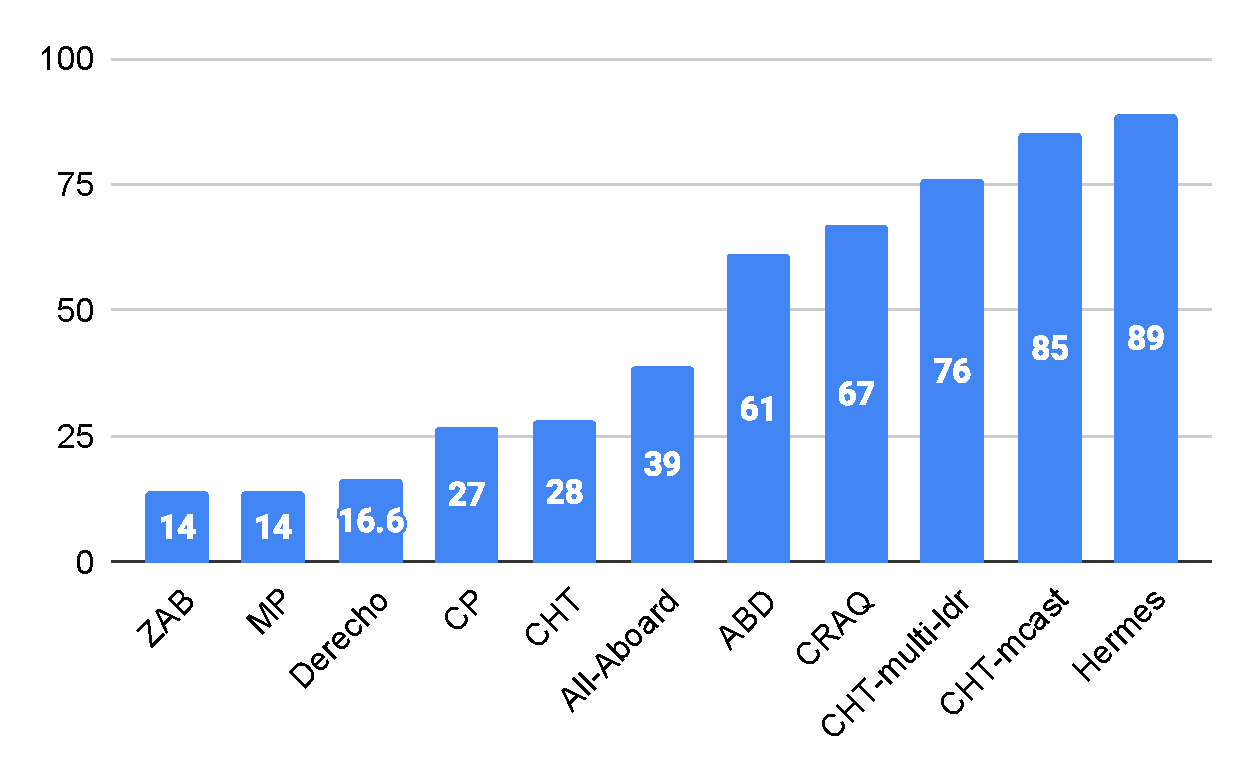
\includegraphics[scale=0.4]{1_figures/Write-only-chart.pdf}
%   \vspace{-0.5em}
  \caption{Write throughput of all protocols [5 nodes]}
%   \vspace{-1.5em}
  \label{fig:write-all}
\end{figure}
% \begin{figure}[t]
  \centering
  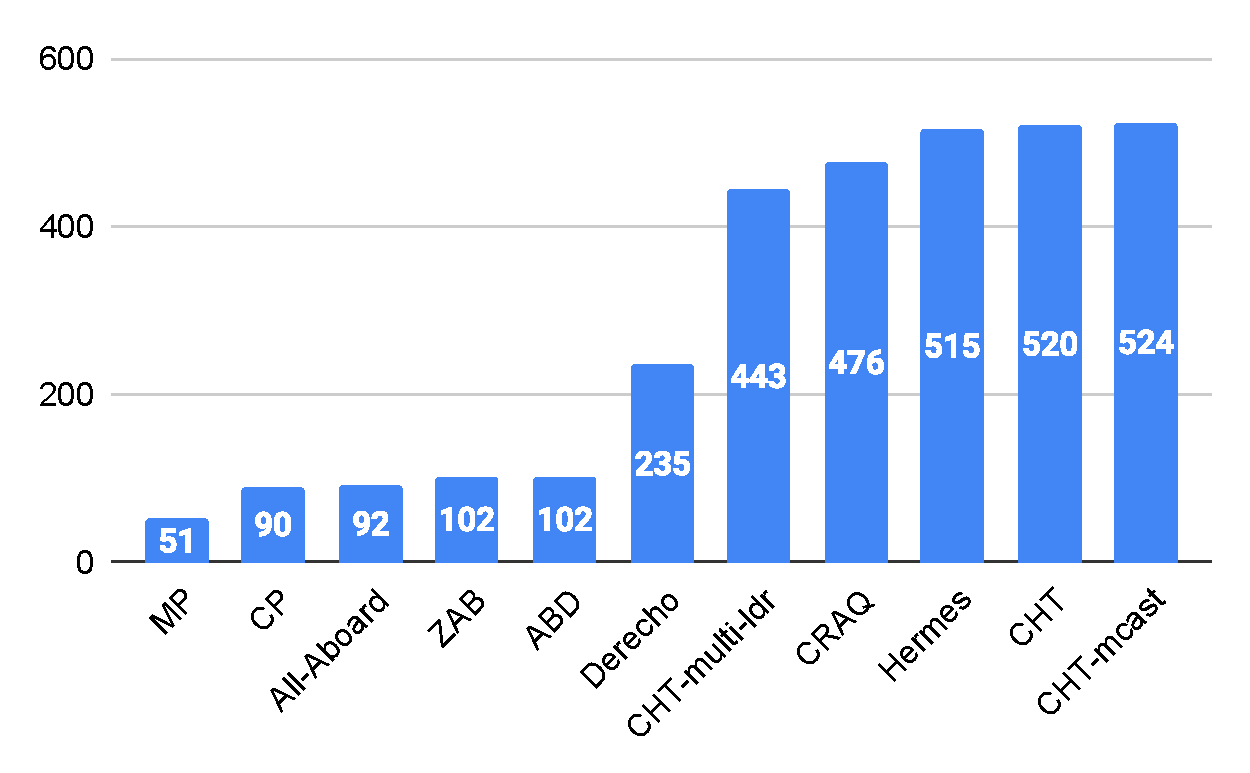
\includegraphics[scale=0.4]{1_figures/5perc-writes.pdf}
%   \vspace{-0.5em}
  \caption{Throughput of all protocols at 95\% reads}
%   \vspace{-1.5em}
  \label{fig:5perc}
\end{figure}


\end{comment}
% 
\y{
\beginbsec{Skewed workloads}
Our evaluation does not investigate the sensitivity of replication protocols under a skewed workload (\eg zipfian distribution~\cite{Novakovic:2016}). This is not an oversight. 

It is possible to apply an optimization where reads and writes to the most popular keys (\ie the \qt{hot keys}) can be combined within each server by leveraging the fact that: 1) 
a server can efficiently keep track of the hot keys~\cite{S-Li:2016, Metwally:2005, Cormode:2008} and 2) at any given moment, a server is expected to be working on multiple requests for each of the hot keys.
This optimization turns skew from problem to opportunity. This is not a surprise: researches have repeatedly observed that skew is a form of locality, and as such it can be leveraged to increase performance~\cite{Priyank:2019,S-Li:2016, A&V:2018, L1:2020}.

Notably, the optimization is equally applicable to all \pnum\ protocols.
Consequently, 
evaluating the protocols without the optimization would paint a false picture, suggesting that protocols suffer under skew, when in reality they can thrive under it. 
However, 
the optimization will take a different shape for each protocol. Therefore, incorporating the optimization to all \pnum\ protocols will require substantial research  
and we leave it for future work.



}








\section{Related Work}
\label{sec:related}

\beginbsec{Related Frameworks}
% There are two alternatives to the functionality offered by \odlib.
Similarly to \odlib, 
Paxi~\cite{Ailijiang:2019} offers a rich interface that enables the fast development of replication protocols. However, Paxi is neither multi-threaded nor \RDMA-enabled.
eRPC~\cite{Kalia:2019} is a general-purpose networking framework offering \RDMA-based RPCs, similarly to \odlib.
However, \odlib\ also provides functionality tailored for replication protocols, such as the smart messages (\S\ref{sec:nw:sm}). 
The reason we did not use eRPC as the networking layer of \odlib, is twofold. 
First, in eRPC, a broadcast requires a separate memcpy for each of the messages. 
In our setup that would result in multiple GBytes/s worth of unnecessary memcpying, for almost all protocols.
Secondly, eRPC would not allow us to use the multicast primitive.

\y{
Finally, G-DUR~\cite{Ardekani:2014b} is a generic middleware that enables the developers to implement and evaluate a large family of distributed transactional protocols.  %that leverage the Deferred Update Replication (DUR)approach.
G-DUR focuses on providing a substrate for transactional protocols that are based on the Deferred Update Replication (DUR) approach. In contrast, \odlib\ focuses on exploring the impact of modern hardware in strongly-consistent replication protocols.
}


\beginbsec{Analysis of replication protocols}
Ailijiang \etal~\cite{Ailijiang:2019} dissect the performance of strongly-consistent replication protocols. Their analysis is complimentary to ours, as they focused on latency and availability on wide-area-networks and geo-replication, while we focus on performance within the datacenter and over modern hardware.
% Renesse \etal~\cite{Renesse:2014}

\y{
\beginbsec{Modern Hardware}
\odlib\ investigates the interplay between protocol-level design decisions and three advances that are described as \emph{modern hardware}: many-core servers, user-level high-bandwidth networking  and high-capacity main memory.
Notably, Szekeres \etal~\cite{Szekeres:2020} also observe the importance of thread-scalability in the era of user-level networking, and propose the Zero-Coordination Principle a guideline to building thread-scalable replicated transactional storage systems. 
% This is complements \odlib, which focuses on the protocol-level actions that hinder thread-scalability.
Furthermore, recent work~\cite{Li:2016-NoPaxos, L1:2020, Zhu:2019, Li:2017, Jin:2017, Jin:2018, Firestone:2018} has investigated the impact of programmable hardware (FPGAs, smart NICs and switches) in deploying storage systems in the datacenter. Such programmable hardware can be used to accelerate the replication protocol. We believe that by uncovering the impact of protocol-level actions on performance our comparison of protocols can serve as a starting point for this endeavor, guiding both the selection of protocols to accelerate and the acceleration process itself.


}

\y{
\beginbsec{Skewed workloads}
Our evaluation does not investigate the sensitivity of replication protocols under a skewed workload (\eg zipfian distribution~\cite{Novakovic:2016}). This is not an oversight. 

It is possible to apply an optimization where reads and writes to the most popular keys (\ie the \qt{hot keys}) can be combined within each server by leveraging the fact that: 1) 
a server can efficiently keep track of the hot keys~\cite{S-Li:2016, Metwally:2005, Cormode:2008} and 2) at any given moment, a server is expected to be working on multiple requests for each of the hot keys.
This optimization turns skew from problem to opportunity. This is not a surprise: researches have repeatedly observed that skew is a form of locality, and as such it can be leveraged to increase performance~\cite{Priyank:2019,S-Li:2016, A&V:2018, L1:2020}.

Notably, the optimization is equally applicable to all \pnum\ protocols.
Consequently, 
evaluating the protocols without the optimization would paint a false picture, suggesting that protocols suffer under skew, when in reality they can thrive under it. 
However, 
the optimization will take a different shape for each protocol. Therefore, incorporating the optimization to all \pnum\ protocols will require substantial research  
and we leave it for future work.



}








\section{Conclusion and Lessons Learned}
\label{sec:conclusion}

The goal of the paper is to uncover the impact of modern hardware on the performance of strongly-consistent replication protocols.
To this end, we presented \odlib, a framework that enables the fast development and deployment of replication protocols over modern hardware. 
Over \odlib, we built and evaluated \pnum\ protocols. 
Extrapolating their results to the entire design space through an informal taxonomy, we provided a characterization of strongly-consistent replication protocols.

On the system side, we experienced first-hand the necessity for a reliable, high-performance framework to design, build and deploy replication protocols. Without it, system-level bugs (networking, KVS etc.) become a black hole for developer time.
In hindsight, this is no surprise: clean interfaces that abstract orthogonal components have been the cornerstone of computer science. %
Nevertheless, 
we were pleasantly surprised to see that we can build and deploy a new protocol in two days (\S\ref{sec:why}). 

When it comes to protocol design, the overarching lesson is that the true limits of a protocol will be uncovered only when all artificially imposed bottlenecks have been removed. 
Plainly, this calls for highly-optimized, multi-threaded and \RDMA-enabled implementations. 
It is very telling that ZAB outperforms Classic Paxos (CP) by more than 2x when both are single-threaded, but the result is inverted when they are multi-threaded. 
The pseudo bottleneck of single-thread implementations conceal ZAB's inefficiencies while holding back CP's capabilities. Multi-threading removes the bottleneck, laying bare the true nature of the protocols.





\begin{acks}
 We would like to thank Boris Grot, the anonymous reviewers and our shepherd Vivien Quema for their valuable comments and feedback. 
 This work was supported in part by EPSRC grant EP/L01503X/1 to The University of Edinburgh, ARM and Microsoft Research through their PhD Scholarship Programs.
\end{acks}




% \clearpage
% \renewcommand{\baselinestretch}{1.0}
% Use the following at camera-ready time to suppress page numbers.
% Comment it out when you first submit the paper for review.
%\thispagestyle{empty}

%%% ACM Bibliography Style
%\bibliographystyle{style/ACM-Reference-Format}
%\bibliography{paper}

%%% IEEE Bibliography Style
%\bibliographystyle{abbrv}
%\bibliography{paper}

%%% USENIX Bibliography Style
% {\footnotesize 
\bibliographystyle{ACM-Reference-Format}
\bibliography{paper}
% }
%\theendnotes

% \appendix
% \section{Appendix}
\label{sec:appendix}




\end{document} 
